% Options for packages loaded elsewhere
\PassOptionsToPackage{unicode}{hyperref}
\PassOptionsToPackage{hyphens}{url}
\PassOptionsToPackage{dvipsnames,svgnames,x11names}{xcolor}
\documentclass[
  11pt,
  a4paper,
]{book}
\usepackage{xcolor}
\usepackage[margin=0.65in]{geometry}
\usepackage{amsmath,amssymb}
\setcounter{secnumdepth}{5}
\usepackage{iftex}
\ifPDFTeX
  \usepackage[T1]{fontenc}
  \usepackage[utf8]{inputenc}
  \usepackage{textcomp} % provide euro and other symbols
\else % if luatex or xetex
  \usepackage{unicode-math} % this also loads fontspec
  \defaultfontfeatures{Scale=MatchLowercase}
  \defaultfontfeatures[\rmfamily]{Ligatures=TeX,Scale=1}
\fi
\usepackage[]{mathpazo}
\ifPDFTeX\else
  % xetex/luatex font selection
\fi
% Use upquote if available, for straight quotes in verbatim environments
\IfFileExists{upquote.sty}{\usepackage{upquote}}{}
\IfFileExists{microtype.sty}{% use microtype if available
  \usepackage[]{microtype}
  \UseMicrotypeSet[protrusion]{basicmath} % disable protrusion for tt fonts
}{}
\makeatletter
\@ifundefined{KOMAClassName}{% if non-KOMA class
  \IfFileExists{parskip.sty}{%
    \usepackage{parskip}
  }{% else
    \setlength{\parindent}{0pt}
    \setlength{\parskip}{6pt plus 2pt minus 1pt}}
}{% if KOMA class
  \KOMAoptions{parskip=half}}
\makeatother
\usepackage{longtable,booktabs,array}
\usepackage{calc} % for calculating minipage widths
% Correct order of tables after \paragraph or \subparagraph
\usepackage{etoolbox}
\makeatletter
\patchcmd\longtable{\par}{\if@noskipsec\mbox{}\fi\par}{}{}
\makeatother
% Allow footnotes in longtable head/foot
\IfFileExists{footnotehyper.sty}{\usepackage{footnotehyper}}{\usepackage{footnote}}
\makesavenoteenv{longtable}
\usepackage{graphicx}
\makeatletter
\newsavebox\pandoc@box
\newcommand*\pandocbounded[1]{% scales image to fit in text height/width
  \sbox\pandoc@box{#1}%
  \Gscale@div\@tempa{\textheight}{\dimexpr\ht\pandoc@box+\dp\pandoc@box\relax}%
  \Gscale@div\@tempb{\linewidth}{\wd\pandoc@box}%
  \ifdim\@tempb\p@<\@tempa\p@\let\@tempa\@tempb\fi% select the smaller of both
  \ifdim\@tempa\p@<\p@\scalebox{\@tempa}{\usebox\pandoc@box}%
  \else\usebox{\pandoc@box}%
  \fi%
}
% Set default figure placement to htbp
\def\fps@figure{htbp}
\makeatother
\setlength{\emergencystretch}{3em} % prevent overfull lines
\providecommand{\tightlist}{%
  \setlength{\itemsep}{0pt}\setlength{\parskip}{0pt}}
\usepackage[most]{tcolorbox}
\usepackage{titling}
\usepackage{amsmath,amssymb}
\usepackage{amsmath}
\usepackage[mathcal]{eucal}
\usepackage[table]{xcolor}
\usetikzlibrary{fit, backgrounds}
\usepackage{arydshln}
\usepackage[most]{tcolorbox}
\usepackage{booktabs}
\usepackage{amsthm}
\usepackage{listings}
\usepackage{tikz}
\usepackage{xcolor}
\usetikzlibrary{matrix}
\usepackage{luacode}
\usepackage{pgfplots}
\pgfplotsset{compat=1.18}
\usetikzlibrary{arrows.meta, positioning}
\renewcommand{\contentsname}{Conteúdo}
\renewcommand{\chaptername}{Capítulo}
\renewcommand*\familydefault{\sfdefault}
\pretitle{\begin{center} 
\includegraphics[width=4in,height=2in]{figures/iseg.png}\LARGE\\}
\usepackage{actuarialsymbol}
\usepackage{booktabs}
\usepackage{longtable}
\usepackage{array}
\usepackage{multirow}
\usepackage{wrapfig}
\usepackage{float}
\usepackage{colortbl}
\usepackage{pdflscape}
\usepackage{tabu}
\usepackage{threeparttable}
\usepackage{threeparttablex}
\usepackage[normalem]{ulem}
\usepackage{makecell}
\usepackage{xcolor}
\usepackage{bookmark}
\IfFileExists{xurl.sty}{\usepackage{xurl}}{} % add URL line breaks if available
\urlstyle{same}
\hypersetup{
  pdftitle={Processos Estocásticos e Aplicações},
  pdfauthor={Nuno M. Brites},
  colorlinks=true,
  linkcolor={blue},
  filecolor={Maroon},
  citecolor={Blue},
  urlcolor={Blue},
  pdfcreator={LaTeX via pandoc}}

\title{Processos Estocásticos e Aplicações}
\usepackage{etoolbox}
\makeatletter
\providecommand{\subtitle}[1]{% add subtitle to \maketitle
  \apptocmd{\@title}{\par {\large #1 \par}}{}{}
}
\makeatother
\subtitle{Licenciatura em Matemática Aplicada à Economia e Gestão}
\author{Nuno M. Brites}
\date{Setembro de 2025}

\usepackage{amsthm}
\newtheorem{theorem}{Teorema}[chapter]
\newtheorem{lemma}{Lema}[chapter]
\newtheorem{corollary}{Corolário}[chapter]
\newtheorem{proposition}{Propriedade}[chapter]
\newtheorem{conjecture}{Conjetura}[chapter]
\theoremstyle{definition}
\newtheorem{definition}{Definição}[chapter]
\theoremstyle{definition}
\newtheorem{example}{Exemplo}[chapter]
\theoremstyle{definition}
\newtheorem{exercise}{Exercício}[chapter]
\theoremstyle{definition}
\newtheorem{hypothesis}{Hipótese}[chapter]
\theoremstyle{remark}
\newtheorem*{remark}{Nota }
\newtheorem*{solution}{Solução }
\begin{document}
\maketitle

{
\hypersetup{linkcolor=}
\setcounter{tocdepth}{2}
\tableofcontents
}
\chapter*{}\label{section}
\addcontentsline{toc}{chapter}{}

\begin{center}
\includegraphics[width=0.4\linewidth]{figures/iseg} \end{center}

\(\,\)

\(\,\)

\(\,\)

\(\,\)

Todas as informações relacionadas com esta UC encontram-se no Fénix.

\(\,\)

Agradeço ao Professor Alfredo Egídio dos Reis (ISEG) a cedência de alguns exercícios presentes neste texto. Agradeço igualmente ao Professor Pedro Soares (ISEG) pela profunda e competente revisão do texto.

Todos os erros e omissões são da minha inteira responsabilidade. Caso detete algum erro ou
gralha, muito agradeço que me informe. Sugestões e comentários também serão muito
bem-vindos.

\(\,\)

Obrigado,

Nuno M. Brites

\href{mailto:nbrites@iseg.ulisboa.pt}{\nolinkurl{nbrites@iseg.ulisboa.pt}}

ISEG, Setembro de 2025

\vfill

\(\,\)

\(\,\)

\(\,\)

\(\,\)

\textbf{Todos os direitos reservados. É expressamente proibida a reprodução, cópia, distribuição, comunicação pública, transformação ou qualquer outra forma de utilização, total ou parcial, dos conteúdos deste sítio, incluindo textos, código e imagens, sem autorização prévia e por escrito do autor. Qualquer utilização não autorizada constitui violação dos direitos de autor e poderá dar lugar à responsabilidade civil e criminal nos termos da lei em vigor.}

2025 \textbar{} Nuno M. Brites \textbar{}
\href{mailto:nbrites@iseg.ulisboa.pt}{\nolinkurl{nbrites@iseg.ulisboa.pt}}

\chapter{Introdução aos processos estocásticos}\label{introducao-aos-processos-estocasticos}

\section{Conceitos fundamentais}\label{conceitos-fundamentais}

Nesta secção procede-se a uma revisão sumária de noções basilares de probabilidade e de variáveis aleatórias. Seguidamente, introduz-se o conceito de processo estocástico, entendido como uma família de variáveis aleatórias definidas sobre um espaço de probabilidade e indexadas por um conjunto de parâmetros, usualmente interpretados como o tempo. Finalmente, analisam-se algumas classes fundamentais de processos estocásticos, em particular os processos com incrementos independentes e estacionários, bem como os processos estacionários em sentido forte e em sentido fraco.

Designa-se, como habitualmente, por \textbf{espaço amostral} o conjunto de todos os resultados possíveis de uma experiência aleatória, representado por \(\Omega\). No que se segue, consideramos que \(\Omega\) é um conjunto não vazio.

\(\,\)

\begin{definition}[Sigma-álgebra]
Uma \(\sigma\)-álgebra é uma família \(\mathcal{F}\) de subconjuntos de \(\Omega\) que satisfaz as seguintes propriedades:

\begin{enumerate}
\def\labelenumi{\roman{enumi})}
\item
  \(\emptyset \in \mathcal{F}\) e \(\Omega \in \mathcal{F}\);
\item
  Se \(A \in \mathcal{F}\), então \(A^c \in \mathcal{F}\), onde \(A^c\) denota o complementar de \(A\) relativamente a \(\Omega\);
\item
  Se \(A_n \subseteq \mathcal{F}, ~n \in \mathbb{N}\), então \(\displaystyle \bigcup_{n \in \mathbb{N}} A_n \in \mathcal{F}\).
\end{enumerate}

Os elementos de \(\mathcal{F}\) designam-se por conjuntos mensuráveis (ou \(\mathcal{F}\)-mensuráveis, para explicitar a \(\sigma\)-álgebra a que pertencem).
\end{definition}

\(\,\)

\begin{definition}[Medida de probabilidade]

Uma medida de probabilidade \(P\) na \(\sigma\)-álgebra \(\mathcal{F}\) é uma função \(P: \mathcal{F} \rightarrow [0,1]\) que satisfaz as seguintes propriedades:

\begin{enumerate}
\def\labelenumi{\roman{enumi})}
\item
  \(P(\emptyset) = 0\);
\item
  \(P(\Omega) = 1\);
\item
  Se \((A_n)_{n \in \mathbb{N}}\) é uma família de conjuntos dois a dois disjuntos em \(\mathcal{F}\), então
  \[P\left(\bigcup_{n \in \mathbb{N}}{A_n}\right)=\sum_{n \in \mathbb{N}}{P(A_n)}.\]
\end{enumerate}

\end{definition}

\(\,\)

\begin{definition}[Espaço de probabilidade]
Um espaço de probabilidade é um terno \((\Omega,\mathcal{F},P),\) onde \(\Omega\) é um conjunto, \(\mathcal{F}\) é uma \(\sigma\)-álgebra em \(\Omega\) e \(P\) é uma medida de probabilidade em \(\mathcal{F}\).

Os elementos de \(\mathcal{F}\) chamam-se acontecimentos; \(P(A), ~A \in \mathcal{F}\), representa a probabilidade do acontecimento \(A\).
\end{definition}

\(\,\)

\begin{definition}[Sigma-álgebra de Borel]
Uma \(\sigma-\)álgebra de Borel, \(\mathcal{B}\), definida num conjunto \(E\) satisfaz as seguintes propriedades:

\begin{itemize}
\item
  \(\emptyset \in \mathcal{B}\) e \(E \in \mathcal{B}\);
\item
  \(\mathcal{B}\) é fechada relativamente ao complementar, isto é,
  \(\forall ~ A \in \mathcal{B}: A^c \in \mathcal{B}\);
\item
  \(\mathcal{B}\) é fechada relativamente à reunião numerável, isto é, se \(A_i \in \mathcal{B}\) para todo \(i \in \mathbb{N}\), então \(\bigcup\limits_{i=1}^{n} A_i \in \mathcal{B}\).
\end{itemize}

Uma \(\sigma-\)álgebra de Borel é um caso particular de uma \(\sigma-\)álgebra e aplica-se aos conjuntos abertos de \(E\). A \(\sigma-\)álgebra de Borel mais comum é a \(\sigma-\)álgebra de Borel em \(\mathbb{R}\), que se denota por \(\mathcal{B}_{\mathbb{R}}\), ou simplesmente \(\mathcal{B}\) caso não existam ambiguidades.
\end{definition}

\(\,\)

\begin{definition}[Variável aleatória]

Seja \((\Omega,\mathcal{F},P)\) um espaço de probabilidade. Diz-se que uma função \(X:\Omega \rightarrow \mathbb{R}\) é uma variável aleatória (v.a.) se
\[
\forall ~ B \in \mathcal{B}: X^{-1}(B) \in \mathcal{F},
\]
onde \(\mathcal{B}\) denota a \(\sigma\)-álgebra de Borel em \(\mathbb{R}\).

Adicionalmente, diz-que \(X\) é \(\mathcal{F}-\)mensurável, ou simplesmente mensurável quando a \(\sigma\)-álgebra associada estiver subentendida.

Em termos gráficos,

\begin{center}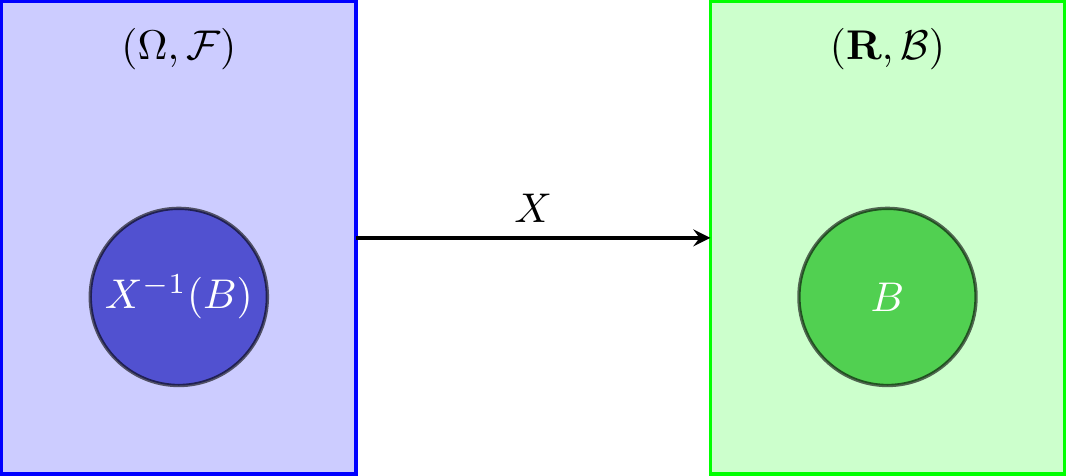
\includegraphics[width=0.6\linewidth]{index_files/figure-latex/fig0-1} \end{center}

\end{definition}

\(\,\)

\begin{theorem}
Seja \(X:\Omega \to \mathbb{R}\) uma variável aleatória. Defina-se
\[
\sigma(X) = \{ X^{-1}(B) : B \in \mathcal{B} \}.
\]
Então, \(\sigma(X)\) é a menor \(\sigma\)-álgebra sobre \(\Omega\) para a qual \(X\) é mensurável. Esta σ-álgebra, que está contida em \(\mathcal{F}\), designa-se por \textbf{σ-álgebra gerada por \(X\)}.
\end{theorem}

\(\,\)

\begin{definition}[Média e variância]
Sejam \((\Omega,\mathcal{F},P)\) um espaço de probabilidade e \(X:\Omega \rightarrow \mathbb{R}\) uma variável aleatória. Define-se o \textbf{valor esperado} (ou média) e a \textbf{variância} de \(X\) da seguinte forma:

\textbf{1. Caso geral (medida de probabilidade \(P\)):}
\[
E(X) = \int_\Omega X \, dP, \quad 
\operatorname{Var}(X) = \int_\Omega (X - E(X))^2 \, dP,
\]
desde que estes integrais existam e sejam finitos.

\textbf{2. Caso discreto:}\\
Se \(X\) assume valores em um conjunto discreto \(\{x_1, x_2, \dots\}\) com probabilidades \(p_i = P(X=x_i)\), então
\[
E(X) = \sum_i x_i \, p_i, \quad 
\operatorname{Var}(X) = \sum_i (x_i - E(X))^2 \, p_i.
\]

\textbf{3. Caso contínuo:}\\
Se \(X\) possui densidade \(f_X(x)\) relativamente à medida de Lebesgue, então
\[
E(X) = \int_{-\infty}^{+\infty} x f_X(x) \, dx, \quad 
\operatorname{Var}(X) = \int_{-\infty}^{+\infty} (x - E(X))^2 f_X(x) \, dx.
\]
\end{definition}

\(\,\)

\begin{definition}

Sejam \((\Omega,\mathcal{F},P)\) um espaço de probabilidade e \(X\) uma variável aleatória definida nesse espaço.

\begin{enumerate}
\def\labelenumi{\roman{enumi})}
\item
  Diz-se que \(X\) é uma variável aleatória de quadrado integrável quando
  \[E(X^2)<+\infty;\]
\item
  O espaço \(L^2\) é o conjunto das variáveis aleatórias de quadrado integrável definidas em \((\Omega,\mathcal{F},P)\);
\item
  A norma \(L^2\) é a norma definida por
  \[\forall ~ X \in L^2:~ ||X||_{L^2} = \left(E(X^2)\right)^{1/2}.\]
\end{enumerate}

\end{definition}

\(\,\)

\begin{remark}
Relativamente à definiçao de espaço \(L^2\), na realidade deveríamos dizer: ``espaço constituído pelas classes de equivalência de variáveis aleatórias\ldots{}'', isto é, para duas variáveis aletórias \(X\) e \(Y\) definidas em \((\Omega,\mathcal{F},P)\), considere-se a relação de equivalência
\[X \sim Y \iff P(X \neq Y)=0\]
e constrói-se o espaço \(L^2\) a partir da classe de equivalência \([X]=\{Y: X \sim Y\}\).
\end{remark}

\(\,\)

\begin{definition}
Seja \((X_n: n \in \mathbb{N})\) uma sucessão de variáveis aleatórias em \(L^2\). Diz-se que \((X_n: n \in \mathbb{N})\) converge para \(X\) em \(L^2\) se
\[||X_n-X||_{L^2}\rightarrow 0 \quad \text{ quando } \quad n \to +\infty,\]
ou, de modo equivalente,
\[E((X_n-X)^2) \to 0 \quad \text{ quando } \quad n \to +\infty.\]
A este tipo de convergência chama-se convergência em média quadrática e representa-se por
\[X_n \xrightarrow{m.q.}X \quad \text{ quando } \quad n \to +\infty\]
ou
\[\mathop{l.i.m.}\limits_{n \to +\infty}X_n=X.\]
\end{definition}

\(\,\)

\begin{definition}

Sejam \(X\) uma variável aleatória e \((X_n : n \in \mathbb{N})\) uma sucessão de variáveis aleatórias definidas no espaço de probabilidade \((\Omega, \mathcal{F}, P)\).

\begin{enumerate}
\def\labelenumi{\roman{enumi})}
\item
  Diz-se que \(X_n\) converge quase certamente (q.c.), ou que converge com probabilidade 1 para \(X\), e denota-se por\\
  \[
  X_n \xrightarrow{q.c.} X \quad \text{ou} \quad \lim_{n \to +\infty} X_n = X \quad q.c.,
  \]\\
  se \(X_n(\omega) \to X(\omega)\) para todo \(\omega \in \Omega \setminus N\), onde \(N \in \mathcal{F}\) é um conjunto de medida nula, isto é, \(P(N) = 0\).
\item
  Diz-se que \(X_n\) converge em probabilidade (ou converge estocasticamente) para \(X\), e denota-se por\\
  \[
  X_n \xrightarrow{P} X \quad \text{ou} \quad P-\lim_{n \to +\infty} X_n = X,
  \]\\
  se, para todo \(\delta > 0\),\\
  \[
  P(|X_n - X| > \delta) \to 0 \quad \text{quando} \quad n \to +\infty.
  \]\\
\end{enumerate}

\end{definition}

\(\,\)

Quando se pretende estudar fenómenos que não têm qualquer evolução, usam-se \textbf{amostras
aleatórias} (repetições de observações i.i.d.'s). Mas, e se estivermos perante \textbf{variáveis
aleatórias} que já se observaram (ou podiam observar) no passado e que poderemos observar
no futuro? Tal ocorre quando pretendemos estudar, por exemplo:

\begin{itemize}
\item
  cotação diária de uma ação na bolsa de valores;
\item
  evolução da taxa de desemprego num dado período;
\item
  número de pessoas que chegam a uma certa fila para serem atendidas;
\item
  evolução da temperatura num local;
\item
  \(\ldots\)
\end{itemize}

Nos casos acima descritos dispomos apenas de uma única observação (chamada \textbf{trajetória}) a
partir da qual se pretende extrair conclusões. Nesta trajetória não existe independência
entre observações. Tipicamente pretendemos fazer:

\begin{itemize}
\item
  previsão de observações futuras;
\item
  identificação do tipo de evolução;
\item
  filtragem (previsão com a ajuda de observações parciais).
\end{itemize}

\(\,\)

\begin{definition}[Processo estocástico]

Um \textbf{processo estocástico} (PE) é uma família de v.a \(\{X_t, ~t \in T\}\), definida sobre o
mesmo espaço de probabilidade \((\Omega, \mathcal{F}, P)\) e assumindo valores num mesmo
espaço mensurável \((E,\mathcal{B})\), onde:

\begin{itemize}
\item
  \(T:\) espaço dos parâmetros (ou do tempo);
\item
  \(\Omega:\) espaço de resultados possíveis;
\item
  \(\mathcal{F}:\) \(\sigma-\)álgebra definida em \(\Omega\);
\item
  \(P:\) medida de probabilidade;
\item
  \(E:\) conjunto de espaço de estados (a definir posteriormente);
\item
  \(\mathcal{B}:\) \(\sigma-\)álgebra de Borel definida em \(E\).
\end{itemize}

\end{definition}

\(\,\)

\begin{remark}
\leavevmode

\begin{itemize}
\item
  Dado um espaço de probabilidade \((\Omega, \mathcal{F}, P)\) e um conjunto arbitrário \(T\),
  um PE é uma função \(X(t,\omega)\) definida em \(T \times \Omega\), tal que, para cada
  \(t \in T\), \(X_t(\omega)\) é uma v.a..
\item
  O conceito de PE generaliza o de v.a. fazendo-a depender de um parâmetros \(t\) com
  domínio em \(T\). Assim, podemos interpretar um PE como uma família ordenada de v.a.'s.
\item
  Para cada \(\omega_0\) fixo, \(\omega_0 \in \Omega\), \(X(\omega_0,t)\) é uma função não
  aleatória de \(t\). Deste modo, um PE pode identificar-se com um sistema que a cada ponto
  \(\omega \in \Omega\), faz corresponder uma função de parâmetro \(t\). Cada uma dessas
  funções diz-se uma trajetória ou realização do processo \(X\).
\end{itemize}

\end{remark}

\(\,\)

\begin{definition}[Trajetória de um processo estocástico]
Chama-se \textbf{trajetória} ou \textbf{realização} de um processo estocástico \(X\) à coleção
\(\{X_t(\omega), t \in T\}\), \(\forall ~ \omega \in \Omega\).
\end{definition}

\(\,\)

\begin{remark}

Em geral \((E,\mathcal{B})=(\mathbb{R}^n, \mathcal{B}_{\mathbb{R}^n})\), onde:

\begin{itemize}
\item
  \(\mathbb{R}^n:\) conjunto dos possíveis valores do processo \(X_t\);
\item
  \(\mathcal{B}_{\mathbb{R}^n}:\) \(\sigma-\)álgebra dos borelianos de \(\mathbb{R}^n\);
\item
  Se \(n=1\) o PE chama-se processo estocástico univariado;
\item
  Se \(n>1\) o PE chama-se processo estocástico multivariado;
\item
  \(t:\) instante onde é feita a observação ou o período relativo a essa observação;
\item
  Se \(E\) for finito ou infinito numerável então \(X\) é um PE de espaço de estados
  discreto;
\item
  Se \(E=\mathbb{R}\) então \(X\) é um PE de valores reais;
\item
  Se \(T\) for finito ou infinito numerável então \(X\) é um PE de tempo discreto (tipicamente
  \(T=\mathbb{N}_0\) ou \(T=\mathbb{Z}\));
\item
  Se \(T\) for infinito não numerável então \(X\) é um PE de tempo contínuo (tipicamente
  \(T=\mathbb{R}^+_0\) ou \(T=\mathbb{R}\)).
\end{itemize}

\end{remark}

\(\,\)

Segue-se um exemplo de uma trajetória de um PE:

\pandocbounded{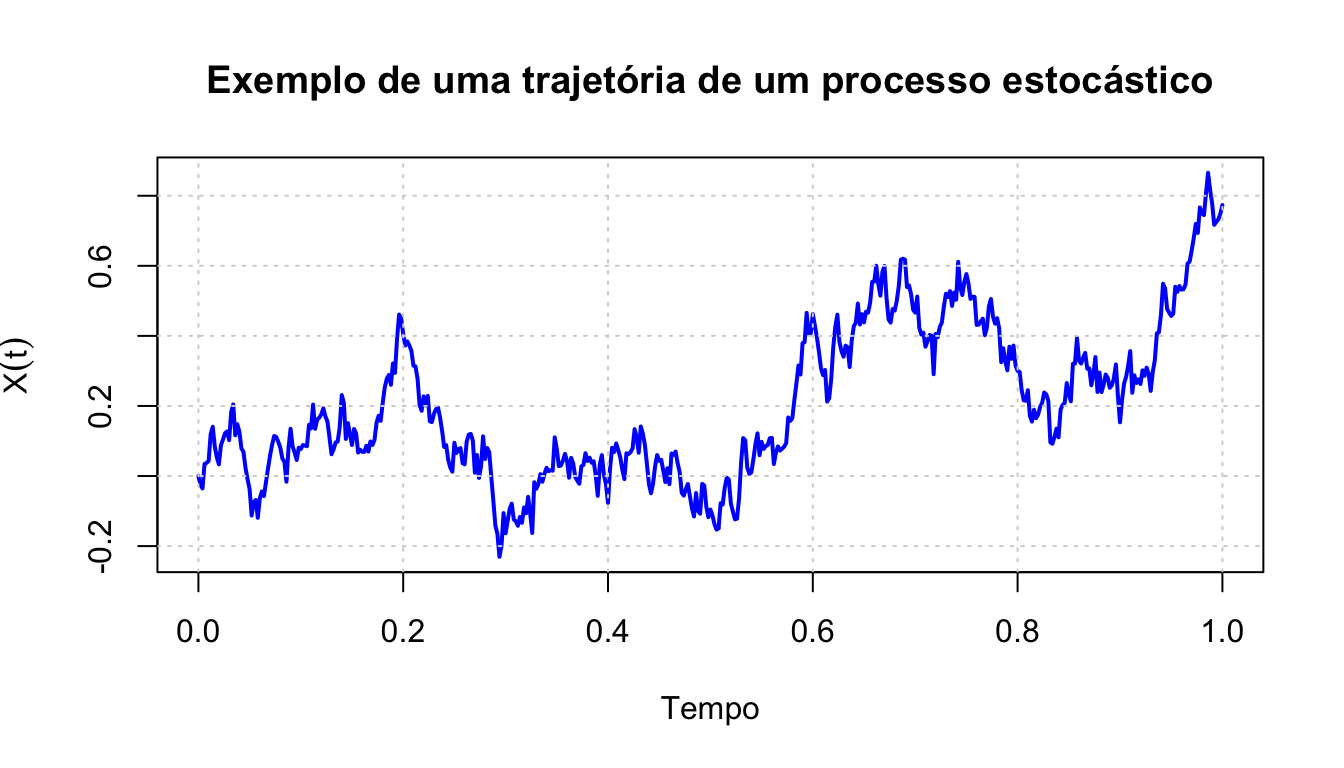
\includegraphics[keepaspectratio]{index_files/figure-latex/simulacao-movimento-browniano-1.pdf}}

\(\,\)

\begin{exercise}

Para cada um dos seguintes processos estocásticos indique o espaço parâmetro e o espaço de estados:

\begin{enumerate}
\def\labelenumi{(\alph{enumi})}
\item
  Sejam \(X_i\) a quantidade de cerveja (em litros) pedida pelo \(i-\)ésimo cliente que entrou num bar e \(N(t)\) o número de clientes que chegaram ao bar até ao instante \(t\). O processo estocástico é
  \[Z_t=\sum\limits_{i=1}^{N(t)}X_i, ~t \geq 0,\]
  onde \(Z_t\) representa a quantidade de cerveja pedida até ao instante \(t\).
\item
  Trinta e seis pontos são escolhidos aleatoriamente no Alaska de acordo com alguma distribuição de probabilidade. Centrado em cada um desses pontos é desenhado um círculo de raio aleatório originando assim uma região \(\Delta\) do Alaska. Seja \(X(A)\) o preço do petróleo extraído no solo da região \(A \cap \Delta\). O processo é
  \[(X(B): ~B \subset Alaska).\]
\item
  Um bebé dorme numa de três posições: (i) de barriga para cima com feição radiante; (ii) enrolada na posição fetal; (iii) na posição fetal, chupando o dedo polegar. Seja \(X_t\) a posição de dormir do bebé no instante \(t\). O processo é \((X_t: ~t\geq 0)\).
\item
  Seja \(X_n\) o estado (ligado ou desligado) de uma fotocopiadora de um escritório ao meio-dia do \(n-\)ésimo dia. O processo é \((X_n: ~ n =1, 2, \dots)\).
\end{enumerate}

\end{exercise}

\(\,\)

\begin{exercise}
\leavevmode

Seja \(\Omega = \{\omega_1, \omega_2, \omega_3, \omega_4\}\) com \(P(\omega_i) = 1/4\), para \(i = 1, 2, 3, 4\). Considere-se o processo estocástico \(\{X(t, \omega): ~ t \geq 0\}\) tal que
\[
X(t, \omega_i) = t \times i, \quad i = 1, 2, 3, 4.
\]

\begin{enumerate}
\def\labelenumi{(\alph{enumi})}
\item
  Classifique o processo em causa;
\item
  Determine a função distribuição de \(X\) para \(t = 1\);
\item
  Indique as trajectórias do processo;
\item
  Determine a função distribuição conjunta de \(\left(X(1), X(2), X(3)\right)\).
\end{enumerate}

\end{exercise}

\(\,\)

\begin{exercise}
\leavevmode

Considere uma sucessão infinita de provas de Bernoulli. Seja
\(X_{t}\) o número de provas até obter um sucesso pela \(t\)-ésima
vez, \(t = 1, 2, \ldots\)

\begin{enumerate}
\def\labelenumi{(\alph{enumi})}
\item
  Defina o exposto como um processo estocástico, indicando o espaço dos parâmetros e dos estados.
\item
  Determine, para cada \(t\), a função de probabilidade de \(X_{t}\).
\item
  Represente graficamente uma trajectória do processo.
\item
  Determine a distribuição conjunta de \((X_{2}, X_{3}, X_{4})\).
\item
  Calcule \(P(X_{4} = x \mid X_{3} = x_{3}, X_{2} = x_{2})\) e \(P(X_{4} = x \mid X_{3} = x_{3})\). Comente o resultado.
\item
  Determine a distribuição da v.a. ``tempo ou número de provas entre dois sucessos de Bernoulli''.
\item
  Determine a distribuição da v.a. ``número de provas necessárias até à ocorrência de dois sucessos consecutivos de Bernoulli''.
\end{enumerate}

\end{exercise}

\section{Tipos clássicos de processos estocásticos}\label{tipos-classicos-de-processos-estocasticos}

\subsection{Processos de incrementos independentes e estacionários}\label{processos-de-incrementos-independentes-e-estacionarios}

\begin{definition}[Processo com incrementos inpedendentes]
\(\{X_t, ~ t \in T\}\) é um PE com \textbf{incrementos independentes} sse
\[\forall ~n \in \mathbb{N}, \forall ~t_1, \ldots,t_n \in T: ~t_1 <t_2<\ldots<t_n \implies X_{t_2}-X_{t_1}, X_{t_3}-X_{t_2},\ldots,X_{t_n}-X_{t_{n-1}}\]
são v.a.'s mutuamente independentes.
\end{definition}

\(\,\)

\begin{definition}[Processo com incrementos estacionários]
\(\{X_t, ~ t \in T\}\) tem \textbf{incrementos estacionários} sse \(\forall ~s, t \in T, ~s<t,\) a
distribuição de \(X_t-X_s\) depende apenas da amplitude \(t-s\).
\end{definition}

\(\,\)

\begin{remark}
Num PE com incrementos estacionários, a distribuição de \(X_{t_{1+h}}-X_{t_1}\) é a mesma de
\(X_{t_{2+h}}-X_{t_2}\), \(\forall ~ t_1,t_2 \in T\) e \(\forall ~ h \in \mathbb{R}_0^+\) tais que \(t_1+h, ~t_2+h \in T.\)
\end{remark}

\(\,\)

Do ponto de vista da modelação, a propriedade de independência de incrementos pode ser
postulada para o modelo quando os resultados obtidos em intervalo de tempo disjuntos forem
independentes. Adicionalmente, a propriedade de estacionariedade de incrementos pode ser
postulada para o modelo quando for plausível que a distribuição de resultados em qualquer
intervalo de tempo depende apenas da amplitude desse intervalo.

\(\,\)

\begin{definition}[Processo de incrementos independentes e estacionários]
Dado um PE \(X:=\{X_t, ~ t \in T\}\), onde \(T\) está munido de uma relação de ordem, \(X\) é um PE
de \textbf{incrementos independentes e estacionários} sse tiver incrementos independentes e
incrementos estacionários.
\end{definition}

\subsection{Processo estocástico real de 2ª ordem}\label{processo-estocastico-real-de-2-ordem}

\begin{definition}[Processo Gaussiano]
Diz-se que \(\{X_t, ~t \in T\}\) é um \textbf{Processo Gaussiano} se
\[
\forall ~n \in \mathbb{N},~ \forall ~t_1, \ldots, t_n \in T, \quad (X_{t_1}, X_{t_2}, \ldots, X_{t_n}) \sim \mathcal{N}_n(\mu, \Sigma),
\]
isto é, qualquer vetor finito de variáveis aleatórias do processo tem distribuição normal multivariada.
\end{definition}

\(\,\)

\begin{definition}[Processo estocástico real de 2ª ordem]
Diz-se que \(\{X_t, ~ t \in T\}\) é um \textbf{processo estocástico real de 2ª ordem} se, e só se,\\
\[
\forall ~t \in T: \; E\!\left(X_t^2\right) < +\infty.
\]

Nestes casos, a descrição do processo faz-se habitualmente em termos dos seus dois primeiros momentos:

\begin{itemize}
\tightlist
\item
  \textbf{função média}: \(m(t) = E(X_t), \quad \forall~t \in T\);
\item
  \textbf{função de covariância}: \(\Gamma(s,t) = \mathrm{Cov}(X_s, X_t), \quad \forall~s,t \in T\).
\end{itemize}

Em geral, a informação fornecida por \(m(t)\) e \(\Gamma(s,t)\) não determina completamente a distribuição do processo. Contudo, no caso particular de um processo Gaussiano, a especificação destes dois primeiros momentos é suficiente para caracterizar completamente o processo.
\end{definition}

\(\,\)

\begin{example}[Ruído Branco Gaussiano]

Chama-se \textbf{Ruído Branco Gaussiano} a um PE \(\{\varepsilon_t, ~t \in T\}\) que satisfaz:

\begin{itemize}
\item
  \(\forall ~t \in T, ~E(\varepsilon_t)=0\);
\item
  \(\forall ~t \in T, ~Var(\varepsilon_t)=\sigma^2\);
\item
  \(\forall ~s, t \in T, s \neq t, ~Cov(\varepsilon_s,\varepsilon_t)=0\);
\item
  \(\forall ~n \in \mathbb{N}, \forall ~t_1, t_2, \ldots, t_n \in T: (\varepsilon_{t_1}, \varepsilon_{t_2}, \ldots, \varepsilon_{t_n})\) é um vetor aleatório Gaussiano.
\end{itemize}

\end{example}

\subsection{Processos estacionários}\label{processos-estacionarios}

\begin{definition}[Processo estacionário em sentido forte]
Diz-se que um PE \(\{X_t,~ t \in T\}\) é \textbf{estacionário em sentido forte} (ou fortemente estacionário) se:
\[\forall~n \in \mathbb{N},~ \forall~t_1, \ldots, t_n \in T,~ \forall~h \in \mathbb{R} \text{ tal que } t_1 + h, \ldots, t_n + h \in T,\]
\[(X_{t_1}, \ldots, X_{t_n}) \buildrel d \over = (X_{t_1+h}, \ldots, X_{t_n+h}),\]
ou seja, a distribuição conjunta de qualquer vetor finito de variáveis do processo é invariante por translação do tempo.
\end{definition}

Como consequência da estacionariedade forte, temos o seguinte Teorema:

\begin{theorem}

Se \(\{X_t, t \in T\}\) é um PE de 2ª ordem e se é fortemente estacionário, então:

\begin{itemize}
\item
  \(E(X_t)=m\), isto é, a média do processo é independente de \(t\);
\item
  \(\forall ~h \in T, ~ \Gamma(t,t+h)=Cov(X_t,X_{t+h})=Cov(X_0,X_h)=\gamma(h)\),
  independente de \(t\).
\end{itemize}

\end{theorem}

\(\,\)

\begin{definition}[Processo estacionário em sentido fraco]

Um PE \(\{X_t, t \in T\}\) é \textbf{estacionário em sentido fraco} (ou estacionário de 2ª ordem),
sse:

\begin{itemize}
\item
  \(\forall ~t \in T, ~E(X^2_t)< + \infty\);
\item
  \(\forall ~t \in T, ~E(X_t)=m\), independente de \(t\);
\item
  \(\forall ~t \in T, \forall ~h \in T,  ~Cov(X_t,X_{t+h})=\gamma(h)\), isto é, a covariância
  apenas depende de \(h\).
\end{itemize}

\end{definition}

\(\,\)

\begin{remark}
A função \(\gamma(h), ~\forall ~ h \in T\), chama-se \textbf{função de autocovariância}. Se \(h=0\),
então \(Cov(X_t,X_{t+h})=Var(X_t)=\gamma(0), ~\forall ~t \in T.\) A esta propriedade chama-se
propriedade da homocedasticidade.
\end{remark}

\(\,\)

Vejamos agora que o Ruído Branco, \(\{\varepsilon_t, ~t \in T\}\), é um exemplo de um PE
estacionário de 2ª ordem:

\begin{example}
\leavevmode

\begin{itemize}
\item
  \(E(\varepsilon_t)=0\);
\item
  \(Var(\varepsilon_t)=\sigma^2 \implies E(\varepsilon^2_t) < + \infty\);
\item
  \(t \neq s, ~Cov(\varepsilon_s,\varepsilon_t)=0, \implies\) independência de \(t\) e de \(s\).
\end{itemize}

Assim,

\[
\gamma(h)=
\begin{cases}
\sigma^2, \quad h=0,\\
0, \quad h \neq 0.
\end{cases}
\] Logo, estão satisfeitas as condições de estacionariedade fraca.

\end{example}

\(\,\)

\begin{remark}[Observação importante]
\[\text{Estacionariedade forte} + E(X_t^2) <+\infty \Rightarrow \text{Estacionariedade fraca}.\]
\[\text{Estacionariedade fraca} \nRightarrow \text{Estacionariedade forte}.\]
\end{remark}

\(\,\)

\begin{example}
Considere o PE \((X_t, ~t \in \mathbb{N})\) onde \(X_t\) tem distribuição de Cauchy, isto é, com
f.d.p. \(f(x)=\dfrac{1}{\pi(1+x^2)}\). Uma vez que não existe \(E(X_t)\), então \(E(X_t^2)\) não
está definido. Assim, o processo é fortemente estacionário mas não é fracamente
estacionário.
\end{example}

\(\,\)

\begin{proposition}[Propriedades da função de autocovariância em processos estacionários]

A função de autocovariância \(\gamma(h)\) goza das seguintes propriedades:

\begin{itemize}
\item
  \(\gamma(h)=\gamma(-h), ~ \forall ~h \in \mathbb{Z}\), isto é, a função de autocovariância é
  par;
\item
  \(\forall ~n \in \mathbb{N}, \forall ~a_j \in \mathbb{R}, \forall ~t_j \in \mathbb{Z}, ~j=1, \ldots,n:\)
  \[\forall~n \in \mathbb{N},~ \forall~a_1, \ldots, a_n \in \mathbb{R},~ \forall~t_1, \ldots, t_n \in \mathbb{Z}, \quad
    \sum_{j=1}^{n} \sum_{k=1}^{n} a_j a_k\, \gamma(t_j - t_k) \geq 0,\]
  isto é, a função de autocovariância define uma forma quadrática não-negativa.
\end{itemize}

\end{proposition}

\(\,\)

\begin{definition}[Função de autocorrelação em processos estacionários]
Seja \(\{X_t, ~ t \in T\}\) um PE estacionário. Chama-se \textbf{função de autocorrelação} à função
\(\rho\) definida por:
\[\rho(h)=Corr(X_t,X_{t+h})=\dfrac{Cov(X_t,X_{t+h})}{\sqrt{V(X_t)}\sqrt{V(X_{t+h})}}=\dfrac{\gamma(h)}{\gamma(0)}.\]
\end{definition}

\(\,\)

\begin{proposition}[Propriedades da função de autocorrelação em processos estacionários]

A função de autocorrelação \(\rho(h)\) goza das seguintes propriedades:

\begin{itemize}
\item
  \(\rho(h)=\rho(-h), \forall ~h \in \mathbb{Z}\), isto é, a função de autocorrelação é
  par;
\item
  \(\forall ~n \in \mathbb{N}, \forall ~a_j \in \mathbb{R}, \forall ~t_j \in \mathbb{Z}, ~j=1, \ldots,n:\)
  \[\sum\limits_{j=1}^{n}\sum\limits_{k=1}^{n} a_ja_k\rho(t_j-t_k) \geq 0,\] isto é,
  trata-se de uma função semi-definida positiva.
\end{itemize}

\end{proposition}

\(\,\)

\begin{exercise}
\leavevmode

Sejam \(X\) e \(Y\) duas variáveis aleatórias com média nula, não correlacionadas e com a mesma variância \(\sigma^2>0\). Considere-se o PE \((Z_t: ~t \in \mathbb{Z})\) definido por:

\[Z_t=f(t) \cdot X + g(t) \cdot Y, \quad t \in \mathbb{Z},\]
onde \(f\) e \(g\) são função determinísticas.

\begin{enumerate}
\def\labelenumi{(\alph{enumi})}
\item
  Encontre expressões para \(f\) e \(g\) de modo a garantir que o processo \((Z_t: ~t \in \mathbb{Z})\) admita variância constante mas não seja necessariamente estacionário em sentido fraco.
\item
  Concretize \(f\) e \(g\) de modo a que \((Z_t: ~t \in \mathbb{Z})\) seja fracamente estacionário.
\end{enumerate}

\end{exercise}

\(\,\)

\begin{exercise}

Seja \(\varepsilon = (\varepsilon_t: ~t \in \mathbb{Z})\) um ruído branco de variância \(\sigma^2 > 0\). Considere os processos estocásticos \(X = (X_t: ~ t \in \mathbb{Z})\) e \(Y = (Y_t: ~ t \in \mathbb{Z})\) definidos do seguinte modo:
\[X_t = \varepsilon_t \quad \text{e} \quad Y_t = (-1)^t \varepsilon_t, \quad \forall ~ t \in \mathbb{Z}.\]

\begin{enumerate}
\def\labelenumi{(\alph{enumi})}
\item
  Prove que \(X\) e \(Y\) são fracamente estacionários.
\item
  Mostre que o processo \((Z_t = X_t + Y_t: ~  t \in \mathbb{Z})\) é um processo não estacionário.
\end{enumerate}

\end{exercise}

\(\,\)

\begin{exercise}

Considere um processo estocástico \(Y = (Y_t: t \in \mathbb{Z})\) tal que \(Y_t = \varepsilon_t - \theta \varepsilon_{t-1}\), \(\theta \in [-1,1]\), onde \((\varepsilon_t: t \in \mathbb{Z})\) é um ruído branco gaussiano de variância \(\sigma^2 > 0\).

\begin{enumerate}
\def\labelenumi{(\alph{enumi})}
\item
  Mostre que \(Y\) é gaussiano.
\item
  Determine a distribuição da variável aleatória \(Y_t, ~\forall ~t \in \mathbb{Z}\).
\item
  Determine a função de autocorrelação de \(Y\).
\item
  O que pode concluir quanto à estacionariedade forte e fraca de \(Y\)?
\end{enumerate}

\end{exercise}

\(\,\)

\begin{exercise}

Seja \(X = (X_t: ~ t \geq 0)\) um processo estocástico, definido sobre o espaço de probabilidade \((\Omega, \mathcal{F}, P)\), tal que, para todo \(t \geq 0\), \(X_t \sim \mathcal{N}(0, t)\), e \(P(X_0 = 0) = 1\).

\begin{enumerate}
\def\labelenumi{(\alph{enumi})}
\item
  Diga em que condições será \(X\) um processo de incrementos independentes e estacionários.
\item
  Supondo que \(X\) é um processo de incrementos independentes e estacionários, mostre que: (i) \(\forall~ t, s \in [0,+\infty[\), com \(t > s\), tem-se que \(X_t - X_s \sim \mathcal{N}(0, |t - s|)\); (ii) \(X\) é um processo gaussiano centrado.
\item
  Considere o processo estocástico \(Y = (Y_t: t \geq 0)\) tal que:
  \[
  Y(t)= 
  \begin{cases}
  t, & X_t \geq 0\\
  -t, & X_t < 0.\\
  \end{cases}
  \]
  Mostre que \(Y\) é um processo estocástico de segunda ordem centrado. Será \(Y\) estacionário em algum sentido? Justifique.
\end{enumerate}

\end{exercise}

\(\,\)

\begin{exercise}

Sejam \(X = (X_t: ~t \in \mathbb{Z})\) e \((\varepsilon_t: ~t \in \mathbb{Z})\) dois processos estocásticos definidos sobre o espaço de probabilidade \((\Omega, \mathcal{F}, P)\), tais que:
\[
\forall ~t \in \mathbb{Z}, \quad X_t = \sum\limits_{j=0}^{+\infty} \left( \frac{4}{5} \right)^j \varepsilon_{t-j}.
\]

\begin{enumerate}
\def\labelenumi{(\alph{enumi})}
\item
  Explique em que condições será \(\varepsilon\) um ruído branco.
\item
  Suponha que \(\varepsilon\) é um ruído branco tal que \(E[\varepsilon_t^2] = 9/50\). (i) Prove que \(X\) é fracamente estacionário e indique as respetivas função média e função de autocovariância; (ii) Suponha agora que \(X\) é um processo gaussiano. Indique a distibuição do vector aleatório \((X_t, X_s), ~ \forall ~ t, s \in \mathbb{Z}\).
\item
  Considere o processo estocástico \(Y = (Y_t: t \in \mathbb{Z})\) tal que:
  \[
  Y_t = 
  \begin{cases}
  1/2, & X_t \geq 0 \\
  -1, & X_t < 0,
  \end{cases}
  \]
  admitindo que \(X\) está nas condições da alínea b) ii). Calcule a função média de \(Y\) e mostre que \(Y\) é fracamente estacionário.
\end{enumerate}

\end{exercise}

\(\,\)

\begin{exercise}

Seja \((\varepsilon_t: t \in \mathbb{Z})\) um ruído branco gaussiano de variância \(\sigma^2>0\). Considere um outro processo estocástico \((Y_t: ~t \in \mathbb{Z})\) definido por:
\[Y_t=\varepsilon_t -\theta \varepsilon_{t-1}-\dfrac{\theta}{2}\varepsilon_{t-2}, \quad \theta \in [-1,1].\]

\begin{enumerate}
\def\labelenumi{(\alph{enumi})}
\item
  Defina processo gaussiano e mostre que \(Y\) é gaussiano.
\item
  Determine a função de autocorrelação do processo \(Y\).
\end{enumerate}

\end{exercise}

\subsection{Martingalas}\label{martingalas}

Do ponto de vista da modelação, as martingalas são apropriadas para modelar fenómenos aleatórios, tais como jogos de azar.

\begin{definition}[Martingala]

Um PE \(\{X_t, ~ t \in T\}\) é uma \textbf{Martingala} sse:

\begin{itemize}
\item
  \(E(\mid X_t \mid) < +\infty;\)
\item
  \(\forall ~n \in \mathbb{N}, ~\forall ~t_1< \ldots < t_{n+1} \in T: E(X_{t_{n+1}} \mid X_{t_1}, \ldots X_{t_n})=X_{t_n}\).
\end{itemize}

\end{definition}

\(\,\)

\begin{example}
Considere-se \(E\) discreto e \(T=\mathbb{N}\). Se interpretarmos \(X_n\) como a fortuna de um jogador após a realização do \(n-\)ésimo jogo, então a 2ª condição da definição anterior estabelece que a fortuna \textbf{esperada} após a \((n+1)-\)ésima partida do jogo é igual à fortuna depois do \(n-\)ésimo jogo, independentemente do que ocorreu anteriormente.
\end{example}

\(\,\)

\begin{remark}

Na definição de Martingala, podemos ainda considerar,

\begin{itemize}
\item
  Submartingalas, quando \(\forall ~n \in \mathbb{N}, ~\forall ~t_1< \ldots < t_{n+1} \in T: E(X_{t_{n+1}} \mid X_{t_1}, \ldots X_{t_n}) \leq X_{t_n}\).
\item
  Supermartingalas, quando \(\forall ~n \in \mathbb{N}, ~\forall ~t_1< \ldots < t_{n+1} \in T: E(X_{t_{n+1}} \mid X_{t_1}, \ldots X_{t_n}) \geq X_{t_n}\).
\end{itemize}

\end{remark}

\(\,\)

\begin{exercise}
\leavevmode

Sejam \(X_0, X_1, \dots\) v.a.'s independentes com média finita e nula e \(S_n=\sum\limits_{i=0}^{n}X_i\). Mostre que o PE \(\{S_n: ~n \in \mathbb{N}_0\}\) é uma Martingala.

\end{exercise}

\(\,\)

\begin{exercise}
\leavevmode

Considere um jogo no qual, em cada jogada, o jogador pode ganhar ou perder um euro, com igual probabilidade. Após \(n\) jogadas o ganho desse jogador é dado por \(S_n=\sum\limits_{i=i}^{n}X_i\), onde \(X_1, X_2, \dots\) são v.a.'s independentes. Mostre que o PE \(\{S_n: ~n \in \mathbb{N}\}\) é uma Martingala.

\end{exercise}

\(\,\)

\begin{exercise}
\leavevmode

Sejam \(X_1, X_2, \dots\) são v.a.'s independentes com média unitária. Mostre que o PE \(\{Z_n: ~n \in \mathbb{N}\}\), definido por
\[Z_n=\prod\limits_{i=1}^{n}X_i\]
é uma Martingala.

\end{exercise}

\(\,\)

\begin{exercise}

Seja \((X_n, ~n=0,1,2,\dots)\) um PE com espaço de estados \(\mathbb{N}_0\), com média unitária para \(n \geq 1\), com incrementos independentes e tal que \(P(X_0=0)=1\).

\begin{enumerate}
\def\labelenumi{(\alph{enumi})}
\item
  O que significa dizer que o processo \(X\) tem incrementos independentes?
\item
  Prove que o processo \((X_n, ~n=0,1,2,\dots)\) é uma Martingala.
\item
  Sabendo que \(Var(X_n)=1\), o que pode afirmar quanto à estacionariedade fraca do processo \((X_n, ~n=0,1,2,\dots)\)?
\end{enumerate}

\end{exercise}

\subsection{Processos de Markov}\label{processos-de-markov}

Os processos de Markov são apropriados na modelação de fenómenos aleatórios cujo comportamento futuro não é alterado pelo conhecimento do seu passado, apenas interessa conhecer o estado presente, ou seja, a probabilidade de que o sistema físico esteja num determinado estado num dado instante \(t\) pode deduzir-se a partir do conhecimento desse estado num instante qualquer anterior e essa probabilidade não depende da ``história'' do sistema antes de \(t\).

\(\,\)

\begin{definition}[Processo de Markov]
Um PE \(\{X_t, t \in T\}\) com espaço de estados \(E\) diz-se um \textbf{processo de Markov} (ou \textbf{Markoviano}) sse \(\forall ~n \in \mathbb{N}, ~\forall ~t_1< \ldots < t_{n+1} \in T, ~\forall ~x_1, \ldots, x_{n+1} \in E, ~\forall ~B \in \mathcal{B}:\)
\[P(X_{t_{n+1}} \in B \mid X_{t_1}=x_1, \ldots X_{t_n}=x_n)=P(X_{t_{n+1}} \in B \mid X_{t_n}=x_n).\]
\end{definition}

\(\,\)

\begin{theorem}
Se \(E\) for discreto e \(T=\mathbb{N}\), a propriedade de Markov da definição anterior é equivalente à seguinte:
\[\forall ~n \in \mathbb{N}, ~\forall ~x_0, \ldots, x_{n+1} \in E: P(X_0=x_0, \ldots, X_n=x_n)>0, \text{tem-se que }\] \[P(X_{n+1}=x_{n+1} \mid X_{0}=x_0, \ldots X_{n}=x_n)=P(X_{n+1}=x_{n+1} \mid X_{n}=x_n).\]
\end{theorem}

\(\,\)

\begin{remark}
Os processos de Markov, como quaisquer processos, são classificados de acordo com a natureza do espaço de estados \(E\) e do espaço dos parâmetros \(T\). Uma classe especial de processos de Markov são as \textbf{Cadeias de Markov} (C.M.): processos de Markov com espaço de estados \(E\) \textbf{discreto}.

Assim, uma cadeia de Markov pode interpretar-se com um PE cujo desenvolvimento se pode considerar como uma série de transições entre valores determinados que têm a propriedade de que a distribuição de probabilidade do estado futuro do processo, sabendo-se que ele está num dado estado, depende apenas deste estado e não do modo de como o processo lá chegou. As C.M. são classificadas em \textbf{discretas} ou \textbf{contínuas}. Nesta UC iremos abordar ambos os casos.
\end{remark}

\chapter{Cadeias de Markov em tempo discreto}\label{cadeias-de-markov-em-tempo-discreto}

\section{Introdução}\label{introducao}

Uma cadeia de Markov em tempo discreto, \(\{X_t, t \in T\}\), é um PE de Markov cujo espaço de estados é \textbf{finito} ou \textbf{infinito numerável}.

\subsection{Conceitos básicos}\label{conceitos-basicos}

\begin{definition}[Cadeia de Markov em tempo discreto]
Um PE em tempo discreto \((X_n, ~n \in \mathbb{N}_0)\) com espaço de estados \(E\) discreto é uma \textbf{C.M. em tempo discreto} sse satisfaz a propriedade de Markov
\[\forall ~n \in \mathbb{N}, ~\forall ~x_0, \ldots, x_{n+1} \in E^{n+1}: P(X_0=x_0, \ldots, X_n=x_n)>0, \text{tem-se que }\] \[P(X_{n+1}=x_{n+1} \mid X_{0}=x_0, \ldots X_{n}=x_n)=P(X_{n+1}=x_{n+1} \mid X_{n}=x_n).\]
\end{definition}

\(\,\)

\begin{exercise}

Seja \((X_n, ~n=1,2,\dots)\) uma sucessão de variáveis aleatórias i.i.d. com distribuição de probabilidade definida por:
\[P(X_n=x)=p(1-p)^x, \quad x=0,1,2,\dots; ~ p \in (0,1).\]
Considere ainda o PE
\[Y=(Y_n=\sum\limits_{i=1}^{n}X_i: ~n=1,2,\dots).\]

\begin{enumerate}
\def\labelenumi{(\alph{enumi})}
\item
  Identifique o espaço de estados de \(Y\).
\item
  Mostre que \(P(Y_{n+1}=y \mid Y_n=x)\) é independente de \(n\).
\item
  Verifique que \(Y\) é uma Cadeia de Markov.
\item
  Calcule \(P(Y_1=y_1, Y_3=y_3)\).
\end{enumerate}

\end{exercise}

\(\,\)

\begin{exercise}

Seja \((X_n, ~n=1,2,\dots)\) uma sucessão de variáveis aleatórias i.d.d. com distribuição de probabilidade definida por:
\[P(X_n=1)=p=1-P(X_n=-1), \quad n=1,2,\dots; ~p \in (0,1).\]
Considere o PE \(S=(S_n: ~n\geq 0)\), conhecido como passeio aleatório simples, definido por:
\[S_0=0 \quad \text{e} \quad S_n=\sum\limits_{i=1}^{n}X_i, ~n=1,2,\dots\]

\begin{enumerate}
\def\labelenumi{(\alph{enumi})}
\item
  Identifique o espaço de estados do processo \(S\).
\item
  Prove que \(S\) é uma Cadeia de Markov para qualquer valor de \(p\).
\item
  Determine para que valores de \(p\), o passeio aleatório \(S\) é uma Martingala.
\item
  Calcule a função de autocovariância do processo \(S\) e verifique se o processo é estacionário em sentido fraco.
\end{enumerate}

\end{exercise}

\(\,\)

Associada a uma C.M. em tempo discreto tem-se a \textbf{função de probabilidade de transição a um passo}:
\[P(X_{n+1}=j \mid X_n=i):=P_{ij}(n,n+1),\]
que representa a probabilidade de \(X_{n+1}\) estar no estado \(j\) no instante \(n+1\) sabendo que no instante \(n\) a cadeia estava no estado \(i\).

Se as probabilidades \(P_{ij}(n,n+1)\) não dependerem de \(n\), então a C.M. em tempo discreto diz-se \textbf{homogénea}. Assim, numa C.M. homogénea observa-se

\[P(X_{n+1}=j \mid X_n=i):=P_{ij},~\forall ~i,j \in E, ~\forall ~n \in \mathbb{N}_0.\]
\(\,\)

\begin{remark}

A expressão \(P(X_{n+1}=j \mid X_n=i):=P_{ij}\):

\begin{itemize}
\item
  representa a probabilidade da cadeia ir do estado \(i\) para o estado \(j\) \textbf{num só passo};
\item
  é independente de \(n\), ou seja, é homogénea no tempo.
\end{itemize}

\end{remark}

\(\,\)

Nesta UC apenas iremos estudar C.M. homogéneas. As probabilidade de transição, \(P_{ij}\), são fundamentais para o estudo da estrutura probabilística das C.M.

\(\,\)

\begin{definition}[Matriz de transição]
Define-se \textbf{Matriz de transição} ou \textbf{Matriz de probabilidade de transição} de uma C.M. homogénea à matriz
\[\mathbb{P}=[P_{ij}]_{~i,j \in E}= \begin{bmatrix}
    P_{00} & P_{01} & \dots & P_{0j}  & \dots \\
    P_{10} & P_{11} & \dots & P_{1j}  & \dots \\
    \vdots & \vdots & \vdots & \vdots & \vdots \\
    P_{i0} & P_{i1} & \dots & P_{ij}  & \dots \\
    \vdots & \vdots & \vdots & \vdots & \vdots \\
\end{bmatrix}, \qquad E=\mathbb{N}_0\]
definida pelas probabilidades de transição \(P_{ij}\) do processo.
\end{definition}

\(\,\)

\begin{remark}

Na matriz de transição \(\mathbb{P}\), observa-se:

\begin{itemize}
\item
  \(0 \leq P_{ij} \leq 1, ~i,j=0,1,\ldots\), uma vez que \(P_{ij}\) representa uma probabilidade;
\item
  \(\sum\limits_{j=0}^{+\infty} P_{ij}=1\), uma vez que \(\sum\limits_{j \in E} P_{ij}=\sum\limits_{j \in E}P(X_{n+1}=j \mid X_n=i)\). Isto quer dizer que a soma dos elementos de cada linha é igual a 1.
\end{itemize}

\end{remark}

\(\,\)

\begin{exercise}

Quatro bolas, duas brancas e duas pretas, são distribuídas em duas caixas \(A\) e \(B\), de tal forma que, em cada caixa, ficam duas bolas. Tira-se uma bola de cada caixa e coloca-se cada uma na caixa oposta. Seja \(X_0\) o número de bolas brancas que existiam inicialmente na caixa \(A\). Para \(n \geq 1\), seja \(X_n\) o número de bolas brancas que existirão na caixa \(A\) depois de se terem efetuado \(n\) trocas de bolas.

\begin{enumerate}
\def\labelenumi{(\alph{enumi})}
\item
  Identifique o espaço de estados.
\item
  Determine a matriz das probabilidades de transição.
\end{enumerate}

\end{exercise}

\(\,\)

\begin{theorem}
Um processo estocástico \((X_t,\, t \in \mathbb{N}_0)\) com espaço de estados \(E\) é uma cadeia de Markov homogénea sse existe uma distribuição inicial de \(X_0\) e uma matriz estocástica \(\mathbb{P} = (P_{ij})_{i,j \in E}\) tais que, para todo \(n\ge 0\) e para todo \((i_0,i_1,\dots,i_n)\in E^{\,n+1}\),
\[
P(X_0=i_0,\; X_1=i_1,\; \ldots,\; X_n=i_n)
= P(X_0=i_0)\,\prod_{k=0}^{n-1} P_{\,i_k i_{k+1}}.
\]

Assim, a probabilidade de observar uma sequência de estados (isto é, a probabilidade conjunta) resulta simplesmente da probabilidade inicial e do produto sucessivo das probabilidades de transição entre estados consecutivos.
\end{theorem}

\(\,\)

\begin{example}
Considere uma CM com valores em \(\{0,1\}\) e com distribuição inicial
\[
\mu = (\mu(0), \mu(1)) = (0.6, \, 0.4),
\]

isto é,
\[
\mu(0)=P(X_0=0)=0.6, \quad \mu(1)=P(X_0=1)=0.4.
\]

Assuma que a matriz de transição é:
\[
\mathbb{P} =
\begin{pmatrix}
0.7 & 0.3 \\
0.2 & 0.8
\end{pmatrix},
\]

onde:

\begin{itemize}
\tightlist
\item
  \(P_{00}=0.7 = P(X_{t+1}=0 \mid X_t=0)\)\\
\item
  \(P_{01}=0.3 = P(X_{t+1}=1 \mid X_t=0)\)\\
\item
  \(P_{10}=0.2 = P(X_{t+1}=0 \mid X_t=1)\)\\
\item
  \(P_{11}=0.8 = P(X_{t+1}=1 \mid X_t=1)\)
\end{itemize}

Por exemplo, a probabilidade conjunta, por aplicação do Teorema acima, é obtida por:
\[
P(X_0=0, X_1=1, X_2=0)
= \mu(0)\, P_{01}\, P_{10}
= P(X_0=0)\, P_{01}\, P_{10}
= 0.6 \times 0.3 \times 0.2
= 0.036.
\]

Outro exemplo:
\[
P(X_0=1, X_1=1, X_2=1, X_3=0)
= \mu(1)\, P_{11}\, P_{11}\, P_{10}
= 0.4 \times 0.8 \times 0.8 \times 0.2
= 0.0512.
\]
\end{example}

\(\,\)

\begin{example}[Passeio aleatório como cadeia de Markov]
Seja \((Y_n)_{n \ge 1}\) uma sequência de variáveis aleatórias i.i.d. com valores em \(\mathbb{Z}\) e distribuição \(p(k) = P(Y_n = k)\), \(k \in \mathbb{Z}\). Seja \(X_0\) a posição inicial, com distribuição \(\mu\).

Definindo
\[
X_n = X_0 + \sum_{m=1}^n Y_m, \quad n \in \mathbb{N}_0,
\]
temos que \((X_n)_{n \in \mathbb{N}_0}\) é uma \textbf{cadeia de Markov homogénea}, com:

\begin{itemize}
\tightlist
\item
  Distribuição inicial: \(\mu(i) = P(X_0 = i)\),\\
\item
  Matriz de transição \(\mathbb{P} = (P_{ij})_{i,j \in \mathbb{Z}}\) dada por
  \[
  P_{ij} = P(X_{n+1} = j \mid X_n = i) = P(Y_{n+1} = j-i) = p(j-i).
  \]
\end{itemize}

Logo, pelo teorema acima, a probabilidade conjunta de qualquer trajetória \((i_0, i_1, \dots, i_n)\) é
\[
P(X_0=i_0, X_1=i_1, \dots, X_n=i_n)
= \mu(i_0) \, P_{i_0 i_1} \cdots P_{i_{n-1} i_n}
= \mu(i_0) \, p(i_1-i_0) \cdots p(i_n - i_{n-1}).
\]

Note-se que o passeio aleatório é um exemplo de uma CM homogénea, em que a matriz de transição é determinada pela distribuição dos incrementos.
\end{example}

\(\,\)

\begin{exercise}
\leavevmode

Mostre que o processo aleatório definido no exemplo anterior é uma C.M. homogénea com matriz de transição com probabilidades
\[P_{xy}=p(y-x), ~\forall ~(x,y) \in \mathbb{Z}.\]

\end{exercise}

\(\,\)

\begin{example}[Passeio aleatório unidimensional com passos -1,0,1]
Trata-se de um caso particular do passeio aleatório unidimensional. Interpretação: uma partícula, no instante \(n\), pode efetuar 3 movimentos:

\begin{itemize}
\tightlist
\item
  deslocar-se para a direita com probabilidade \(p\);
\item
  deslocar-se para a esquerda com probabilidade \(q\);
\item
  manter-se na mesma posição com probabilidade \(r\).
\end{itemize}

Se \(X_n\) representar a posição da partícula ao fim de \(n\) movimentos, tem-se
\[
X_n = X_0 + \sum_{i=1}^n Y_i,
\]
onde
\[
Y_i =
\begin{cases}
1, & \text{deslocamento para a direita},\\
-1, & \text{deslocamento para a esquerda},\\
0, & \text{sem deslocamento}.
\end{cases}
\]

\begin{itemize}
\tightlist
\item
  \((Y_n, n \in \mathbb{N})\): sucessão de variáveis aleatórias independentes (representa os incrementos).\\
\item
  \((X_n, n \in \mathbb{N}_0)\): passeio aleatório, isto é, uma CM homogénea com espaço de estados \(\mathbb{Z}\) e matriz de transição \(\mathbb{P}\):
  \[
  P_{ij} = P(X_n = j \mid X_{n-1}=i) =
  \begin{cases}
  p, & j=i+1,\\
  q, & j=i-1,\\
  r, & j=i.
  \end{cases}
  \]
\end{itemize}

Aqui, \(P_{ij}=p(j-i)\) representa a distribuição de probabilidade dos incrementos \(Y_n\). Tipicamente considera-se \(p=q=0.5\) e \(r=0\).
\end{example}

\(\,\)

\begin{remark}
Notação:
\[P^m_{ij}=P(X_{n+m}=j \mid X_n=i)\]
representa a probabilidade de, em \(m\) passos, a cadeia de Markov homogénea passar do estado \(i\) para o estado \(j\).
\end{remark}

\(\,\)

\begin{theorem}
Seja \(\mathbb{P}=[P_{ij}]\) a matriz de transição a um passo de uma C.M. \((X_n, ~n \in \mathbb{N}_0)\). Então,
\[P^m_{ij}=\sum\limits_{k=0}^{+\infty}P_{ik}^r ~ P_{kj}^s,\]
onde \((r,s) \in \mathbb{N}_0^2\) tal que \(r+s=m\) e \(P_{ij}^0=1\) se \(i=j\), e \(P_{ij}^0=0\) se \(i \neq j\).

Este teorema mostra-nos como calcular probabilidades de transição em vários passos de uma cadeia de Markov. Em vez de irmos diretamente de \(i\) para \(j\) em \(m\) passos, podemos ``partir o caminho'' num estado intermédio \(k\): primeiro percorrem-se \(r\) passos até \(k\), e depois mais \(s\) passos de \(k\) até \(j\), com \(r+s=m\). A soma sobre todos os possíveis estados intermédios \(k\) garante que estamos a considerar todos os caminhos possíveis, refletindo a ideia fundamental da multiplicação de probabilidades em cadeias de Markov.
\end{theorem}

\(\,\)

\begin{exercise}
\leavevmode

Considere \(m=2\) e prove o Teorema anterior.

\end{exercise}

\(\,\)

\begin{theorem}[Equações de Chapman-Kolmogorov]
O Teorema anterior pode ser re-escrito como
\[P^{m+n}_{ij}=\sum\limits_{k \in E}P_{ik}^m ~ P_{kj}^n, \quad \forall ~i,j \in E.\]
Assim, \(P_{i,j}^m\) representa o elemento \((i,j)\) da matriz potência de ordem \(m\) de \(\mathbb{P}\).
\end{theorem}

\section{Classificação de estados de uma C.M.}\label{classificacao-de-estados-de-uma-c-m}

Torna-se importante o estudo limite de \(P_{i,j}^n\) quando \(n \to +\infty\). Espera-se que a influência do estado inicial \(i\) diminua com o tempo, e que o limite de \(P_{i,j}^n\) quando \(n \to +\infty\) seja independente de \(i\).

Para se poder analisar o comportamento assintótico do processo, vamos introduzir alguns critérios de classificação de estados de uma C.M.. Consideremos, no que se segue, uma C.M. \((X_n, n \in \mathbb{N}_0)\) com matriz de transição \(\mathbb{P}=[P_{i,j}], ~i,j \in E\).

\(\,\)

\begin{definition}[Estado acessível]

Diz-se que o estado \(j \in E\) é \textbf{acessível} a partir do estado \(i \in E\), se para algum \(n \in \mathbb{N}_0\) se observa \(P_{ij}^n>0\). Representação:

\begin{figure}

{\centering 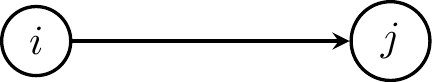
\includegraphics[width=0.25\linewidth]{index_files/figure-latex/fig1-1} 

}

\caption{Estado acessível}\label{fig:fig1}
\end{figure}

\end{definition}

\(\,\)

\begin{definition}[Estados em comunicação]

Se dois estados \(i,j \in E\) são acessíveis um relativamente ao outro, diz-se que intercomunicam ou que estão \textbf{em comunicação}. Representação:

\begin{figure}

{\centering 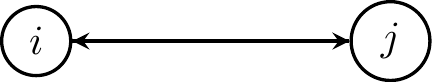
\includegraphics[width=0.25\linewidth]{index_files/figure-latex/fig2-1} 

}

\caption{Estados em comunicação}\label{fig:fig2}
\end{figure}

\end{definition}

\(\,\)

\begin{remark}
Se dois estados \(i,j \in E\) não comunicam, então:
\[\forall ~n \in \mathbb{N}_0, ~P_{ij}^n=0 ~\vee ~ P_{ji}^n=0.\]
\end{remark}

\(\,\)

\begin{theorem}
A intercomunicação dos estados define uma relação de equivalência.
\end{theorem}

\(\,\)

\begin{exercise}
\leavevmode

Mostre o Teorema anterior. Sugestão: mostre que a intercomunicação entre estados é reflexiva, simétrica e transitiva.

\end{exercise}

\(\,\)

\begin{remark}
A relação de equivalência do último Teorema induz uma partição do conjunto de todos os estados em classes de equivalência. Dentro de cada classe todos os estados comunicam entre si.
\end{remark}

\(\,\)

\begin{example}
Considere a seguinte matriz de transição, com \(E=\{0,1,2,\dots,r\}\), de um passeio aleatório:
\[\mathbb{P}= \begin{bmatrix}
    1 & 0 & 0 & 0  & \dots & 0 & 0 \\
    q & 0 & p & 0  & \dots & 0 & 0 \\
    0 & q & 0 & p  & \dots & 0 & 0 \\
    \dots & \dots & \dots & \dots  & \dots & \dots & \dots \\
    0 & 0 & 0 & 0  & q & 0 & p \\
    0 & 0 & 0 & 0  & \dots & 0 & 1 \\
\end{bmatrix}.\]
A relação de equivalência de comunicação induz as classes:
\[\{0\}, ~ \{1,2,\dots,r-1\}, ~\{r\},\]
donde se conclui que: do estado \(0\) só se pode ir para o estado \(0\); todos os estados \(1,2,\dots,r-1\) comunicam entre si; do estado \(r\) só se pode ir para o estado \(r\). Para \(r=5\), isto é, 6 estados, a matriz de transição é:
\[
\mathbb{P} =
\begin{bmatrix}
1 & 0 & 0 & 0 & 0 & 0 \\
q & 0 & p & 0 & 0 & 0 \\
0 & q & 0 & p & 0 & 0 \\
0 & 0 & q & 0 & p & 0 \\
0 & 0 & 0 & q & 0 & p \\
0 & 0 & 0 & 0 & 0 & 1 \\
\end{bmatrix}
\]
e a representação gráfica é:

\begin{center}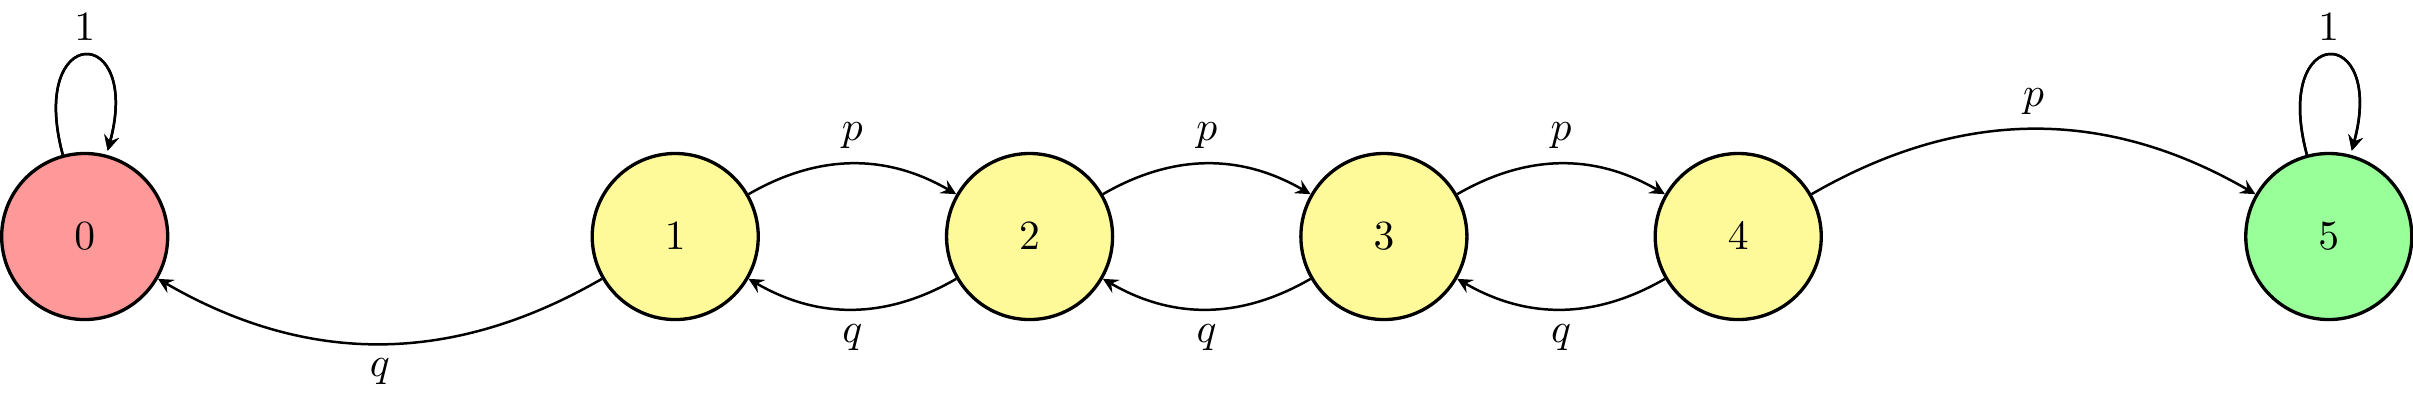
\includegraphics[width=0.9\linewidth]{index_files/figure-latex/fig3-1} \end{center}

As classes de equivalência estão representadas por cores.
\end{example}

\(\,\)

\begin{definition}[Período]
Chama-se \textbf{período} do estado \(i\), e representa-se por \(d(i)\), ao máximo divisor comum de todos os inteiros \(n\geq 1\) tais que \(P_{ii}^n > 0\), isto é,
\[d(i)=\text{m.d.c.}(n \geq 1: P_{ii}^n >0).\]
Convenção: se \(\forall ~n \geq 1, P_{ii}^n=0\), então \(d(i)=0\).
\end{definition}

\(\,\)

\begin{example}
\leavevmode

\begin{enumerate}
\def\labelenumi{\arabic{enumi}.}
\tightlist
\item
  Considere a matriz de transição
  \[
  \mathbb{P} = \begin{bmatrix}
  0 & 1 \\
  1 & 0
  \end{bmatrix}.
  \]
\end{enumerate}

\begin{itemize}
\tightlist
\item
  Se começarmos no estado \(1\), no passo seguinte vamos sempre para \(2\).\\
\item
  Só é possível regressar a \(1\) em \(2,4,6,\dots\) passos.
\end{itemize}

Portanto, o período de \(1\) (e também de \(2\)) é \(d(1)=d(2)=2\).

\begin{enumerate}
\def\labelenumi{\arabic{enumi}.}
\setcounter{enumi}{1}
\tightlist
\item
  Considere a matriz de transição
  \[
  \mathbb{P} = \begin{bmatrix}
  0.5 & 0.5 \\
  0.5 & 0.5
  \end{bmatrix}.
  \]
\end{enumerate}

\begin{itemize}
\tightlist
\item
  Se começarmos no estado \(1\), já no passo seguinte podemos ficar em \(1\) (probabilidade \(0.5\)).\\
\item
  Também conseguimos regressar em \(2\) passos, \(3\) passos, etc.
\end{itemize}

Portanto, o período de \(1\) (e também de \(2\)) é \(d(1)=d(2)=1\).

\end{example}

\(\,\)

\begin{remark}
Dois estados em comunicação têm o mesmo período, isto é,

\[i \longleftrightarrow j \iff d(i)=d(j).\]
\end{remark}

\(\,\)

\begin{exercise}
Determine o período dos estados do exemplo 2.4.
\end{exercise}

\(\,\)

\begin{exercise}
Considere a C.M. de espaço de estados finito com matriz de transição
\[
\mathbb{P} =
\begin{bmatrix}
0 & 1 & 0 & \dots & 0 \\
0 & 0 & 1 & \dots & 0 \\
\vdots & \vdots & \vdots & \vdots & \vdots \\
0 & 0 & 0 & \dots & 1 \\
1 & 0 & 0 & \dots & 0  \\
\end{bmatrix}, \quad E=\{0,1,\dots,n-1\}.
\]
Mostre que \(d(i)=n, ~\forall ~n \in E.\)
\end{exercise}

\(\,\)

\begin{definition}[Estado aperiódico. Cadeia aperiódica.]
Um estado diz-se \textbf{aperiódico} se tem período um. A cadeia é \textbf{aperiódica} se todos os estados acessíveis entre si (isto é, na mesma classe de comunicação) são aperiódicos.
\end{definition}

\(\,\)

\begin{definition}[Tempo mínimo de passagem]
Seja \(T_{ij}\) a variável aleatória que representa o \textbf{tempo (mínimo) de primeira passagem} do estado \(i\) ao estado \(j\),
\[
T_{ij} = \inf \{ n \ge 1 : X_n = j \mid X_0 = i \}.
\]

A função de probabilidade de \(T_{ij}\), representa a \textbf{probabilidade da primeira vez que a cadeia atinge \(j\) exatamente no passo \(n\)}, com ínício em \(i\), isto é,
\[
f_{ij}^n = P(T_{ij} = n), \quad n \ge 1.
\]

Em particular,
\[
f_{ij}^1 = P_{ij}, \text{ para } i \neq j.
\]

Para \(n \ge 2\) e \(i \neq j\), \(f_{ij}^n\) satisfaz a \textbf{relação de recorrência}:
\[
f_{ij}^n = \sum_{k \in E \setminus \{j\}} P_{ik} \, f_{kj}^{\,n-1}.
\]

Isto significa que, para chegar a \(j\) pela primeira vez ao fim de \(n\) passos, a cadeia deve ir primeiro para um estado \(k \neq j\) e depois chegar a \(j\) a partir de \(k\) em \(n-1\) passos.
\end{definition}

\(\,\)

\begin{theorem}

Para todo \(n \in \mathbb{N}\), as probabilidades de transição \(P_{ij}^n\) podem ser expressas em função das probabilidades de primeira passagem \(f_{ij}^k\), do seguinte modo:
\[
P_{ij}^n = \sum_{k=1}^n f_{ij}^k \, P_{jj}^{\,n-k},
\]

onde:

\begin{itemize}
\item
  \(f_{ij}^k\) representa a probabilidade de atingir \(j\) \textbf{pela primeira vez} exatamente no instante \(k\);
\item
  \(P_{jj}^{\,n-k}\) representa a probabilidade de estar em \(j\) nos \(n-k\) instantes restantes, após o primeiro encontro no instante \(k\);
\item
  Somando sobre todos os possíveis instantes \(k = 1,2,\dots,n\), obtemos a probabilidade de estar em \(j\) ao fim de \(n\) instantes.
\end{itemize}

\end{theorem}

\(\,\)

\begin{example}
Considere uma cadeia com estados \(\{0,1\}\) e matriz de transição
\[
\mathbb{P} =
\begin{bmatrix}
0.5 & 0.5 \\
0.2 & 0.8
\end{bmatrix}.
\]

Queremos calcular \(P_{01}^2\), ou seja, a probabilidade de estar em 1 ao fim de 2 passos, partindo de 0. Pela aplicação do teorema anterior,

\[P_{01}^2 = f_{01}^1 \cdot P_{11}^1 + f_{01}^2 \cdot P_{11}^0=f_{01} \cdot P_{11} + f_{01}^2 \cdot 1.\]

\begin{itemize}
\item
  Probabilidades de primeira passagem:
  \[
  f_{01} = P_{01}=0.5, \quad f_{01}^2 = P_{00} \times f_{01} =0.5 \cdot 0.5 = 0.25.
  \]
\item
  Probabilidades de permanência em 1:
  \[
  P_{11} = 0.8, \quad P_{11}^0 = 1.
  \]
\item
  Finalmente,
  \[
  P_{01}^2 = f_{01} \cdot P_{11} + f_{01}^2 = 0.5 \cdot 0.8 + 0.25  = 0.65.
  \]
\end{itemize}

Este exemplo mostra como as \textbf{probabilidades de primeira passagem} \(f_{ij}^k\) determinam a evolução da cadeia ao longo de \(n\) passos.
\end{example}

\(\,\)

\begin{definition}[Estado recorrente e transitório]

Seja
\[
T_{ii} = \inf \{ n \ge 1 : X_n = i \},
\]
o \textbf{tempo de retorno} ao estado \(i\), ou seja, o número de passos até regressar a \(i\) pela primeira vez.

\begin{itemize}
\item
  O estado \(i\) diz-se \textbf{recorrente} se
  \[
  P(T_{ii} < +\infty) = 1,
  \]
  isto é, regressa-se a \(i\) em tempo finito com probabilidade 1.
\item
  O estado \(i\) diz-se \textbf{transitório} se
  \[
  P(T_{ii} < +\infty) < 1,
  \]
  isto é, existe uma probabilidade positiva de nunca mais regressar a \(i\).
\end{itemize}

\end{definition}

\(\,\)

\begin{theorem}[Critérios de recorrência/transitoriedade]
Seja \(P_{ii}^n = P(X_n=i \mid X_0=i)\) e \(f_{ii}^n = P(T_{ii}=n \mid X_0=i)\), onde \(T_{ii}\) é o tempo mínimo de retorno a \(i\). Então:

\begin{itemize}
\item
  O estado \(i\) é \textbf{recorrente} sse a probabilidade de regressar a \(i\) em algum instante é igual a 1, ou seja,
  \[
  \sum_{n=1}^{+\infty} f_{ii}^n = P(T_{ii}<\infty \mid X_0=i) = 1.
  \]
\item
  O estado \(i\) é \textbf{recorrente} sse o tempo de retorno a \(i\) é finito com probabilidade 1:
  \[
  P(T_{ii} < +\infty \mid X_0=i) = 1.
  \]
\item
  O estado \(i\) é \textbf{recorrente} sse a soma das probabilidades de \textbf{estar em \(i\) ao longo de todos os instantes} é infinita:
  \[
  \sum_{n=1}^{+\infty} P_{ii}^n = +\infty.
  \]
\end{itemize}

Caso contrário, o estado \(i\) é \textbf{transitório}.

Além disso, se \(i \longleftrightarrow j\) e \(i\) é recorrente, então \(j\) também é recorrente.
\end{theorem}

\(\,\)

\begin{remark}

Consequências imediatas:

\begin{itemize}
\item
  numa classe de equivalência, todos os estados são recorrentes ou todos são transitórios;
\item
  os estados recorrentes estão organizados em classes de comunicação que são fechadas.
\end{itemize}

\end{remark}

\(\,\)

\begin{definition}[Classificação de estados recorrentes]

Defina-se o tempo médio de retorno
\[
\mu_i = E[T_{ii}] = \sum_{n=1}^{+\infty} n f_{ii}^n.
\]

Um estado recorrente \(i\) é:

\begin{itemize}
\item
  \textbf{recorrente positivo} se \(\mu_i < +\infty\);
\item
  \textbf{recorrente nulo} se \(\mu_i = +\infty\);
\item
  \textbf{recorrente ergódico} se for recorrente positivo e aperiódico.\\
\end{itemize}

\end{definition}

\(\,\)

\begin{definition}[Cadeia de Markov irredutível]
Uma cadeia de Markov com espaço de estados \(E\) diz-se \textbf{irredutível} se, para quaisquer \(i, j \in E\), existe \(n \geq 1\) tal que
\[
P_{ij}^n > 0.
\]
Ou seja, todos os estados comunicam entre si.
\end{definition}

\(\,\)

Segue-se um pequeno resumo das principais propriedades e critérios de classificação dos estados de uma C.M. homogénea:

\(\,\)

\begin{longtable}[]{@{}
  >{\raggedright\arraybackslash}p{(\linewidth - 4\tabcolsep) * \real{0.2750}}
  >{\raggedright\arraybackslash}p{(\linewidth - 4\tabcolsep) * \real{0.5417}}
  >{\raggedright\arraybackslash}p{(\linewidth - 4\tabcolsep) * \real{0.1833}}@{}}
\toprule\noalign{}
\begin{minipage}[b]{\linewidth}\raggedright
Estado / Propriedade
\end{minipage} & \begin{minipage}[b]{\linewidth}\raggedright
Critério principal
\end{minipage} & \begin{minipage}[b]{\linewidth}\raggedright
Observações adicionais
\end{minipage} \\
\midrule\noalign{}
\endhead
\bottomrule\noalign{}
\endlastfoot
\textbf{Recorrente} & \(P(T_{ii} < +\infty) = 1\) & Regressa a \(i\) com probabilidade 1 \\
& \(\sum_{n=1}^{\infty} f_{ii}^n = 1\) & Soma das probabilidades de primeira passagem \\
& \(\sum_{n=1}^{\infty} P_{ii}^n = +\infty\) & Soma das probabilidades de visita \\
\textbf{Transitório} & \(P(T_{ii} < +\infty) < 1\) & Existe probabilidade positiva de nunca regressar \\
& \(\sum_{n=1}^{\infty} f_{ii}^n < 1\) & \\
& \(\sum_{n=1}^{\infty} P_{ii}^n < +\infty\) & \\
\textbf{Recorrente positivo} & \(\mu_i = \sum_{n=1}^{\infty} n f_{ii}^n < +\infty\) & Tempo médio de recorrência finito \\
\textbf{Recorrente nulo} & \(\mu_i = \sum_{n=1}^{\infty} n f_{ii}^n = +\infty\) & Tempo médio de recorrência infinito \\
\textbf{Recorrente ergódico} & Recorrente positivo e aperiódico & Permite aplicação de resultados de ergodicidade \\
\textbf{Cadeia irredutível} & \(\forall i,j\in E, \exists n \ge 1: P_{ij}^n>0\) & Todos os estados comunicam entre si \\
\end{longtable}

\(\,\)

\begin{example}
Considere a cadeia com espaço de estados \(\{0,1,2\}\) e matriz de transição
\[
\mathbb{P} =
\begin{bmatrix}
0 & 1 & 0 \\
0 & 0 & 1 \\
1 & 0 & 0
\end{bmatrix}.
\]

Esta cadeia é irredutível porque, partindo de qualquer estado, é possível atingir qualquer outro estado num número finito de passos, com probabilidade positiva. Por exemplo:

\[0 \longrightarrow 1 \longrightarrow 2 \longrightarrow 0,\]
o que permite circular por todos os estados.

Adicionalmente, todos os estados são recorrentes positivos (verifique!).
\end{example}

\(\,\)

\begin{theorem}
Numa cadeia de Markov irredutível com espaço de estados finito ou infinito numerável, verifica-se que:\\
-- ou todos os estados são transitórios;

-- ou todos são recorrentes nulos;

-- ou todos são recorrentes positivos.
\end{theorem}

\(\,\)

\begin{exercise}
Seja \(X_0, X_1, X_2, \dots\) uma sucessão de variáveis aleatórias i.i.d.'s tal que:
\[P(X_i=-1)=P(X_i=1)=0.5, \quad i=0,1,2,\dots.\]

\begin{enumerate}
\def\labelenumi{(\alph{enumi})}
\tightlist
\item
  Prove que \((X_n: ~n \in \mathbb{N}_0)\) é uma C.M. homogénea com matriz de transição
\end{enumerate}

\[\mathbb{P}=
\begin{bmatrix}
0.5 & 0.5  \\
0.5 & 0.5  \\
\end{bmatrix}.\]

\begin{enumerate}
\def\labelenumi{(\alph{enumi})}
\setcounter{enumi}{1}
\item
  Determine a probabilidade de que o processo \((X_n: ~n \in \mathbb{N}_0)\), partindo do estado 1, volte a atingir este estado, pela primeira vez, num número par de passos.
\item
  Considere o PE \((Y_n: ~n \in \mathbb{N})\) definido por:
\end{enumerate}

\[
Y_n=
\begin{cases}
X_{n-1} \cdot X_{n+1}, & n \text{ par}\\
X_{n}, & n \text{ ímpar}
\end{cases}.
\]

Verifique se \(Y\) é um ruído branco e, em caso afirmativo, identifique a sua variância. Prove que \(Y\) não é uma C.M.
\end{exercise}

\(\,\)

\begin{exercise}

Considere uma estação de táxis, onde de \(s\) em \(s\) segundos chega um táxi. Se não existem clientes a ser servidos, o táxi parte de imediato, chegando outro \(s\) segundos depois. Caso contrário, os clientes vão sendo atendidos por ordem de chegada, havendo sempre um período de tempo constante de \(s\) segundos entre cada serviço. Durante esse período de tempo podem, no entanto, chegar novos clientes. Suponhamos que o número de chegadas ao \(n-\)ésimo período de tempo é uma variável aleatória \(Z_n\) cuja distribuição é independente do período em que ocorrem as chegadas, e é dada por
\[P(\text{k clientes chegarem num intervalo de tempo entre 2 chegadas consecutivas de táxi})= a_k,\]
onde \(a_k \geq 0, ~\forall ~k \in \mathbb{N}_0\), e \(\sum\limits_{k=0}^{+\infty}a_k=1\).

O estado do sistema no início do \((n+1)-\)ésimo período de tempo entre duas chegadas consecutivas de táxi é definido pelo número de clientes que esperam para serem atendidos, sendo esse número representado por \(X_n, ~n \in \mathbb{N}_0\).

\begin{enumerate}
\def\labelenumi{(\alph{enumi})}
\item
  Prove que \(\{X_n, ~n \in \mathbb{N}_0\}\) é uma C.M. homogénea. Indique os respetivos espaço de estados e matriz de transição.
\item
  Sabendo que no início de um determinado intervalo a fila tem zero clientes, qual a probabilidade de o sistema voltar a atingir este estado (pela primeira vez) ao fim de três chegadas de táxis?
\end{enumerate}

\end{exercise}

\(\,\)

\begin{exercise}

Seja \(\{Y_i^{(n)} : i, n \in \mathbb{N} \}\) uma família de variáveis aleatórias independentes e identicamente distribuídas com distribuição binomial \(B(2; 0.5)\).

Considere um processo estocástico \(\{X_n\}_{n \in \mathbb{N}_0}\) definido por:
\[
X_0 = a, ~\text{ com } a \in \mathbb{N} \text{ fixo, e para todo } n \geq 1:
\quad X_n =
\begin{cases}
\sum\limits_{i=1}^{X_{n-1}} Y_i^{(n)}, & \text{se } X_{n-1} \geq a. \\
a, & \text{se } X_{n-1} < a
\end{cases}
\]

\begin{enumerate}
\def\labelenumi{(\alph{enumi})}
\item
  Identifique o espaço de estados do processo \(X\).
\item
  Prove que \(X\) é uma C.M. homogénea e identifique a matriz de transição.
\end{enumerate}

\end{exercise}

\(\,\)

\begin{exercise}

Determinado ser vivo produz, durante a sua vida, um número de descendentes \(Y\) de acordo com uma distribuição dada por:
\[\forall ~k \in \mathbb{N}_0, ~P(Y=k)=\dfrac{\lambda^k}{k!}e^{-\lambda}, \quad \lambda >0 \text{ constante}.\]
A cada indivíduo \(i\) da população associamos uma v.a. \(Y_i=\) número de descendentes do indivíduo \(i\). Para cada \(n \in \mathbb{N}_0\), define-se a v.a. \(X_n\) que representa o tamanho da população na geração de ordem \(n\). Considere o PE \((X_n: ~n \in \mathbb{N}_0)\).

\begin{enumerate}
\def\labelenumi{(\alph{enumi})}
\item
  Prove que \((X_n: ~n \in \mathbb{N}_0)\) é uma C.M. homogénea.
\item
  Calcule a probabilidade de existirem \(k \in \mathbb{N}_0\) indivíduos na geração de ordem \(n+2\), sabendo que na geração de ordem \(n\) existiam \(j \in \mathbb{N}_0\).
\end{enumerate}

\end{exercise}

\(\,\)

\begin{exercise}

Considere lançamentos repetidos de um dado honesto. Seja \(X_n\) o máximo dos números que ocorreram nos \(n\) primeiros lançamentos.

\begin{enumerate}
\def\labelenumi{(\alph{enumi})}
\item
  Indique o espaço de estados da C.M. \((X_n: ~n \in \mathbb{N})\) e a respetiva matriz de transição.
\item
  Determine \(P(X_i=i), ~i=1,2,\dots,6\) e \(P(X_2=3)\).
\item
  Desenhe o grafo da cadeia, classifique os seus estados, e analise o tipo de recorrência.
\item
  Verifique que a cadeia é aperiódica.
\end{enumerate}

\end{exercise}

\(\,\)

\begin{exercise}
Seja \((X_n: ~n \in \mathbb{N})\) uma C.M. com espaço de estados \(E=\mathbb{N}_0\) e probabilidades de transição \(P_{ij}\) tais que:
\[P_{k0}=\dfrac{1}{k+2} \quad \text{e} \quad P_{k,k+1}=\dfrac{k+1}{k+2}.\]
Mostre que a cadeia é irredutível.
\end{exercise}

\(\,\)

\begin{exercise}

Seja \((Z_n: ~n \in \mathbb{N}_0)\) uma C.M. homogénea com espaço de estados \(E=\mathbb{N}_0\) e probabilidades de transição:
\[\mathbb{P}= \begin{bmatrix}
    1-a_0 & a_0 & 0 & 0  & \dots  \\
    1-a_1 & 0 & a_1 & 0  & \dots  \\
    1-a_2 & 0 & 0 & a_2  & \dots  \\
    \dots & \dots & \dots & \dots  & \dots  \\
\end{bmatrix}, \quad 0<a_i<1, ~i=0,1,2,\dots\]

\begin{enumerate}
\def\labelenumi{(\alph{enumi})}
\item
  A cadeia dada é irredutível e aperiódica? Justifique.
\item
  Determine a probabilidade \(f_{00}^n\) de que a cadeia, partindo do estado 0, volte novamente a esse estado, pela primeira vez, em \(n\) passos. De seguida, mostre que:
  \[\sum\limits_{n=1}^{M+1}f_{00}^n=1-\prod\limits_{i=0}^{M}a_i.\]
\item
  Atendendo aos resultados das alíneas anteriores, enuncie, em termos dos \(a_i\)'s, uma condição necessária e suficiente para que todos os estados sejam recorrentes. Justifique a sua resposta.
\end{enumerate}

\end{exercise}

\(\,\)

\begin{exercise}

Uma dada empresa identificou seis estados associados ao comportamento diário dos seus colaboradores: \(0,1,2,3,4,5\). As transições de estado para estado podem ser modeladas por uma C.M. com matriz de transição:
\[\mathbb{P}= \begin{bmatrix}
    1 & 0 & 0 & 0 & 0 & 0  \\
    0.5 & 0 & 0.5 & 0 & 0 & 0  \\
    0.1 & 0 & 0.5 & 0.3 & 0 & 0.1  \\
    0 & 0 & 0 & 0.7 & 0.1 & 0.2  \\
    0.3 & 0 & 0 & 0.3 & 0.4 & 0  \\
    0 & 0 & 0 & 0 & 0 & 1  \\
\end{bmatrix}.\]

\begin{enumerate}
\def\labelenumi{(\alph{enumi})}
\item
  Desenhe o grafo de \(\mathbb{P}\).
\item
  Identifique os estados transitórios e os estados recorrentes.
\end{enumerate}

\end{exercise}

\subsection{Decomposição do espaço de estados}\label{decomposicao-do-espaco-de-estados}

Agora pretendemos decompor o espaço de estados de uma cadeia de Markov finita em subclasses. O objetivo é estudar propriedades da cadeia pela análise das propriedades de cada classe separadamente.

\(\,\)

\begin{definition}[Classe fechada]
Uma \textbf{classe fechada} é uma classe de comunicação \(C\) tal que, se \(i \in C\) e \(P_{ij} > 0\), então \(j \in C\), ou seja, a cadeia nunca pode sair de \(C\) depois de entrar.
\end{definition}

\(\,\)

Coloca-se agora a questão: como encontrar todos os estados que pertencem a uma mesma classe de comunicação (e, em particular, a uma classe fechada)? Seguem-se os passos:

\begin{itemize}
\item
  \textbf{Passo 1:} inclui-se em \(C\) todos os estados \(j\) para os quais \(P_{ij}>0\), isto é, \(i \longrightarrow j\);
\item
  \textbf{Passo 2:} inclui-se em \(C\) todos os estados \(k\) para os quais existe \(j \in C\) com \(P_{jk}>0\), isto é, \(j \longrightarrow k\) para algum \(j \in C\) (propriedade da transitividade);
\item
  \textbf{Passo 3:} repetir o Passo 2 até não se poder incluir mais estados em \(C\);
\item
  \textbf{Passo 4:} verificar se algum estado de \(C\) tem transições para fora.

  \begin{itemize}
  \tightlist
  \item
    Se não tiver, \(C\) é uma \textbf{classe fechada}.\\
  \item
    Caso contrário, \(C\) é apenas uma \textbf{classe de comunicação} (não fechada).
  \end{itemize}
\end{itemize}

Nota: se começarmos num estado \textbf{transitório} e aplicarmos o algoritmo, o conjunto construído acabará por conduzir a uma \textbf{classe fechada}. Assim, as classes fechadas são precisamente os \textbf{menores subconjuntos} do espaço de estados obtidos pela aplicação do algoritmo a todos os estados.

O resultado seguinte permite uma decomposição do espaço de estados de uma cadeia de Markov, chamada \textbf{decomposição canónica}.

\begin{theorem}[Decomposição canónica]

Seja \(\mathbb{P}\) a matriz de transição de uma C.M. com espaço de estados \(E\). Então, \(E\) pode ser decomposto numa união (finita ou infinita enumerável) da forma:
\[
E = T \cup C_1 \cup C_2 \cup \dots,
\]
onde:

\begin{itemize}
\item
  \(T\) é o conjunto dos estados transitórios;
\item
  \(C_1, C_2, \dots\) são classes de comunicação disjuntas, fechadas e constituídas apenas por estados recorrentes.
\end{itemize}

Para cada \(j \in C_a\), a probabilidade de atingir um estado \(k \in E\) num número finito de passos é dada por:

\[
\sum_{n=1}^{+\infty} f_{jk}^{n} =
\begin{cases}
1, & \text{se } k \in C_a, \\
0, & \text{se } k \notin C_a,
\end{cases}
\]

onde \(f_{jk}^{n} = P(X_n = k, X_1 \neq k, \dots, X_{n-1} \neq k \mid X_0 = j)\) é a probabilidade de atingir \(k\) pela primeira vez no instante \(n\), começando em \(j\).

Adicionalmente, reordenando os estados de forma conveniente, a matriz de transição \(\mathbb{P}\) pode ser escrita na forma em blocos:
\[
\mathbb{P} =
\begin{bmatrix}
R & S \\
0 & Q
\end{bmatrix},
\]
onde:

\begin{itemize}
\item
  \(R\) descreve as transições entre estados em \(T\);
\item
  \(S\) descreve as transições de \(T\) para as classes \(C_1, C_2, \dots\);
\item
  \(Q\) é uma matriz bloco-diagonal com submatrizes \(P_1, P_2, \dots\), onde cada \(P_a = [P_{ij}]_{i,j \in C_a}\) representa as transições internas em cada classe recorrente.
\end{itemize}

\end{theorem}

\(\,\)

\begin{remark}

A decomposição canónica do espaço de estados de uma C.M. é muito útil para analisar as propriedades da cadeia, como a recorrência e a transitoriedade dos estados, bem como a classificação dos estados em classes de comunicação. Em particular, quando o espaço de estados \(E\) de uma C.M. é finito, a classificação dos estados pode fazer-se da seguinte forma:

\begin{itemize}
\item
  Passo 1: decompor \(E\) em classes de equivalência (classes de comunicação);
\item
  Passo 2: identificar quais dessas classes são fechadas;
\item
  Passo 3:

  \begin{itemize}
  \item
    em cada classe fechada, todos os estados são recorrentes positivos (porque a classe é finita e fechada);
  \item
    nas classes não fechadas, todos os estados são transitórios.
  \end{itemize}
\end{itemize}

\end{remark}

\(\,\)

\begin{example}
Considere-se uma C.M com espaço de estados \(E=\{1, 2,\dots, 7\}\) e com matriz de transição
\[
\mathbb{P} =
\begin{bmatrix}
0 & 0 & 1 & 0 & 0 & 0 & 0  \\
0 & 1/3 & 0 & 0 & 0 & 0 & 2/3  \\
0 & 0 & 1/2 & 0 & 1/2 & 0 & 0  \\
0 & 1/2 & 0 & 1/2 & 0 & 0 & 0 \\
1/3 & 0 & 1/3 & 0 & 1/3 & 0 & 0  \\
0 & 0 & 0 & 0 & 0 & 1 & 0 \\
1/4 & 1/4 & 0 & 0 & 0 & 0 & 1/2   \\
\end{bmatrix}.
\]

\begin{itemize}
\tightlist
\item
  O grafo associado à matriz \(\mathbb{P}\) é:
\end{itemize}

\begin{center}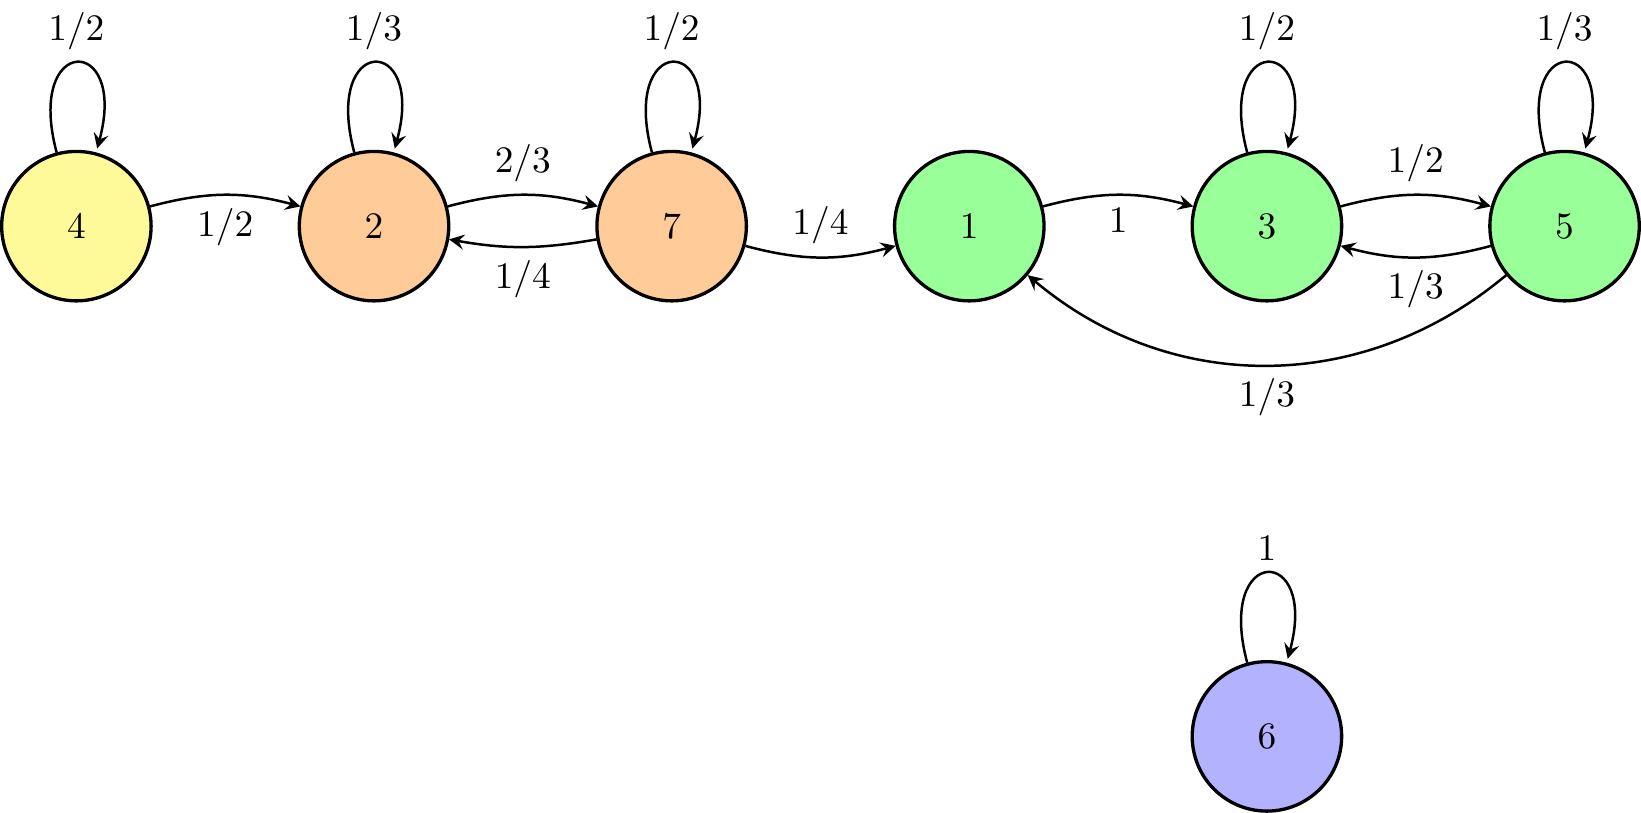
\includegraphics[width=0.9\linewidth]{index_files/figure-latex/fig4-1} \end{center}

\begin{itemize}
\item
  Classes de equivalência (partição de \(E\) com base na relação de comunicação \(i \longrightarrow j\)):
  \[\{1,3,5\}, \{2,7\}, \{4\}, \{6\}.\]
\item
  Classes fechadas (classes de equivalência sem saída):
  \[\{1,3,5\}, \{6\}.\]
\item
  Estados recorrentes positivos (estados em classes fechadas finitas):
  \[1,3,5,6.\]
\item
  Estados transitórios (estados que podem sair da sua classe, ou que não são atingidos novamente):
  \[2,4,7.\]
\item
  Decomposição (separação entre transitórios e classes recorrentes):
  \[E=T \cup C_1 \cup C_2=\{2,4,7\} \cup \{1,3,5\} \cup \{6\}.\]
\item
  A matriz de transição pode ser reescrita como:
\end{itemize}

\[
\mathbb{P} =
\left[
\begin{array}{c:ccc:ccc}
\color{red}{1} & 0 & 0 & 0 & 0 & 0 & 0  \\ \hdashline
0 & \color{blue}{0} & \color{blue}{1} & \color{blue}{0} & 0 & 0 & 0  \\
0 & \color{blue}{0} & \color{blue}{1/2} & \color{blue}{1/2} & 0 & 0 & 0 \\
0 & \color{blue}{1/3} & \color{blue}{1/3} & \color{blue}{1/3} & 0 & 0 & 0  \\ \hdashline
\color{green}{0} & \color{orange}{0} & \color{orange}{0} & \color{orange}{0} & \color{pink}{1/3} & \color{pink}{0} & \color{pink}{2/3}  \\
\color{green}{0} & \color{orange}{0} & \color{orange}{0} & \color{orange}{0} & \color{pink}{1/2} & \color{pink}{1/2} & \color{pink}{0}  \\
\color{green}{0} & \color{orange}{1/4} & \color{orange}{0} & \color{orange}{0} & \color{pink}{1/4} & \color{pink}{0} & \color{pink}{1/2}  
\end{array}
\right]
=
\left[
\begin{array}{ccc}
\color{red}{P_1} & \textbf{0} & \textbf{0} \\
\textbf{0} & \color{blue}{P_2} & \textbf{0} \\
\color{green}{Q_1} & \color{orange}{Q_2} & \color{pink}{Q_3}
\end{array}
\right],
\]
onde \(P_i\) representa a matriz de probabilidades de transição da classe \(C_i\) e \(Q_i\) é a matriz associada a estados de transição. Nota: para re-escrever a matriz usou-se a permutação \((6,1,3,5,2,4,7)\).
\end{example}

\section{Probabilidades de absorção em estados recorrentes}\label{probabilidades-de-absorcao-em-estados-recorrentes}

Um dos cálculos de interesse na teoria das cadeias de Markov está relacionado com o tempo (ou número de transições) necessário, para que, a cadeia partindo de algum estado inicial, \textbf{atinja algum estado terminal de interesse}.

Este assunto está muitas vezes associado ao problema da determinação de \textbf{probabilidades de absorção}, com a seguinte formulação:

\begin{itemize}
\item
  Seja \(E=T \cup C_1 \cup C_2 \cup \dots\) a decomposição canónica do espaço de estados \(E\), onde \(T\) é definido pelos estados transitórios da cadeia, e \(C_a\), \(a=1,2,\dots\), são classes fechadas e recorrentes.
\item
  Se a cadeia parte de um estado recorrente em \(C_a\), nunca mais deixará \(C_a\) (\(C_a\) é fechada).
\item
  Se a cadeia parte de um estado transitório em \(T\), a cadeia poderá ser absorvida por uma das classes \(C_a\).
\end{itemize}

Nestas circunstâncias estamos interessados nas probabilidades de absorção.

\begin{definition}
Seja \(C := \bigcup\limits_a C_a\) a união das classes fechadas de estados recorrentes, e seja \(T\) o conjunto de estados transitórios. Seja \(S\) a variável aleatória definida por
\[
S := \min\{n \geq 1 : X_n \in C\},
\]
isto é, o instante da primeira entrada numa classe recorrente, partindo de um estado transitório.

Dado \(X_0 = i\), com \(i \in T\), o valor
\[
a_{ij} := P(X_S = j \mid X_0 = i), \quad j \in C,
\]
representa a probabilidade de a cadeia, partindo de \(i\), ser absorvida no estado recorrente \(j\).

Esta quantidade é chamada \textbf{probabilidade de absorção} do estado transitório \(i\) no estado recorrente \(j\).
\end{definition}

\(\,\)

\begin{theorem}[Probabilidades de absorção]
Sejam \(E=T \cup C_1 \cup C_2 \cup \dots\) a decomposição canónica do espaço de estados \(E\) e \(C = \bigcup\limits_a C_a\) a união das classes fechadas de estados recorrentes.

Para cada par \((i,j) \in T \times C\), a \textbf{probabilidade de absorção} no estado \(j\), partindo de \(i\), é dada por
\[
a_{ij} = P_{ij} + \sum_{k \in T} P_{ik} \, a_{kj},
\]
onde \(P_{ik}\) são as probabilidades de transição de 1 passo da matriz \(\mathbb{P}\).

\textbf{Interpretação:} a cadeia pode ser absorvida no estado \(j \in C\) de forma imediata (via \(P_{ij}\)) ou, caso isso não ocorra, pode passar para um estado intermédio \(k \in T\), a partir do qual será absorvida em \(j\).
\end{theorem}

\(\,\)

\begin{example}
\leavevmode

\begin{itemize}
\item
  Em jogos de azar: a probabilidade de eventualmente ganhar ou perder tudo.
\item
  Em processos sociais: a probabilidade de uma família atingir e permanecer num certo nível social.
\item
  Em biologia: a probabilidade de uma espécie ou gene acabar por se fixar ou extinguir.
\end{itemize}

\end{example}

\(\,\)

\begin{example}
Num estudo no Reino Unido, após a Segunda Guerra Mundial, sobre a mobilidade social entre gerações foram identificados 3 níveis: 1 - superior, 2 - médio e 3 - inferior. Foram estimadas as probabilidades condicionais de um filho pertencer a uma classe social (nível superior, médio, ou inferior) mediante o nível social dos pais ser superior, médio ou inferior. Os resultados são apresentados na tabela seguinte:

\begin{tabular}{cccc}
\toprule
\multicolumn{1}{c}{ } & \multicolumn{3}{c}{Filho} \\
\cmidrule(l{3pt}r{3pt}){2-4}
Pai & Superior & Médio & Inferior\\
\midrule
Superior & 1.00 & 0.0 & 0.00\\
Médio & 0.20 & 0.6 & 0.20\\
Inferior & 0.05 & 0.5 & 0.45\\
\bottomrule
\end{tabular}

Admitamos que as transições entre classes de gerações sucessivas é uma família que pode ser considerada como transições de uma cadeia de Markov.

\begin{enumerate}
\def\labelenumi{\arabic{enumi}.}
\item
  Qual a probabilidade de um neto de uma família com nível médio (estado 2) seja o primeiro descendente a ser considerado com um nível social superior (estado 1), isto é, qual o valor de \(f_{21}^2\)?
\item
  Qual a probabilidade de que, em alguma geração, de uma família com nível social inferior (estado 3), seja atingida pela primeira vez o nível superior (estado 1)?
\end{enumerate}

\textbf{Solução}

A matriz de transição é dada por

\[
\mathbb{P} =
\begin{bmatrix}
1 & 0 & 0   \\
0.2 & 0.6 & 0.2  \\
0.05 & 0.5 & 0.45 \\
\end{bmatrix}, \quad E = \{1,2,3\} = T \cup C,
\]

onde:

\begin{itemize}
\item
  \(C = \{1\}\) (classe fechada).
\item
  \(T = \{2,3\}\) (estados transitórios).
\end{itemize}

O grafo é

\begin{center}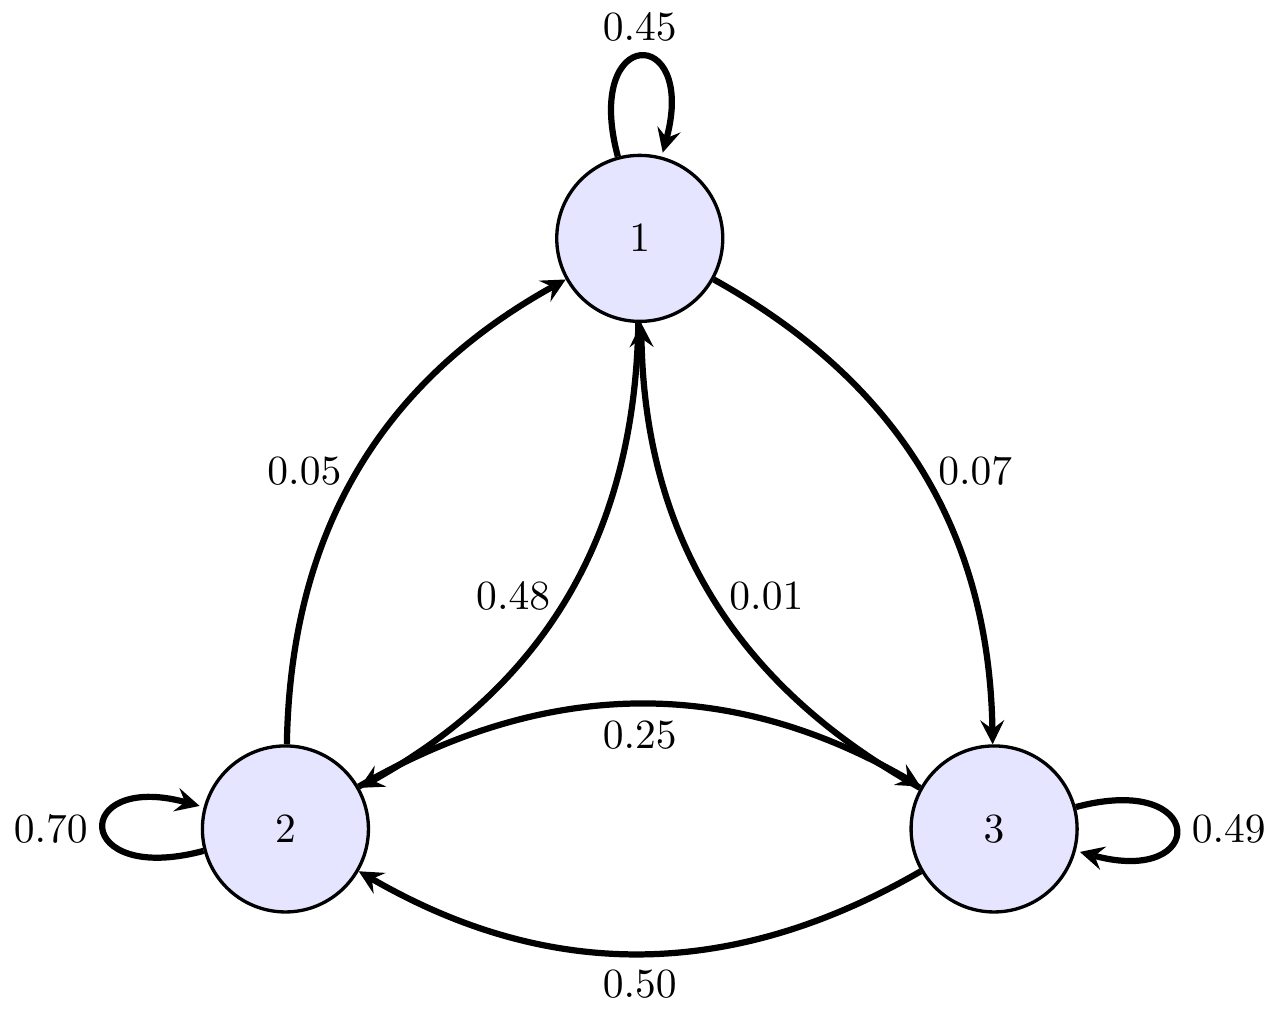
\includegraphics[width=0.6\linewidth]{index_files/figure-latex/fig5-1} \end{center}

\begin{enumerate}
\def\labelenumi{\arabic{enumi}.}
\item
  Pretende-se determinar a probabilidade de, começando no estado 2, o primeiro momento em que a cadeia entra no estado 1 seja no instante 2. Para tal, iremos usar a probabilidade de primeira passagem do estado 2 para o estado 1 em 2 passos, isto é,
  \begin{eqnarray*}
  f_{21}^2 &=& P(X_2=1, X_1 \neq 1 \mid X_0=2) \\
        &=& P(X_2=1, X_1 = 2 \mid X_0=2)+P(X_2=1, X_1 = 3 \mid X_0=2)\\
        &=& \sum\limits_{k \neq 1} P_{2k}P_{k1}\\
        &=& P_{22}P_{21}+P_{23}P_{31}\\
        &=& 0.6 \times 0.2 + 0.2 \times 0.05\\
        &=& 0.13.
  \end{eqnarray*}
\item
  Nesta questão, estamos interessados no cálculo do tempo necessário para que a cadeia, partindo de um estado inicial (``nível social inferior''), atinja um estado recorrente (``nível superior''). Podemos, portanto, utilizar as probabilidades de absorção e aplicar o Teorema anterior. Assim,
\end{enumerate}

\[a_{31}=P_{31}+\sum\limits_{k \in T} P_{3k}a_{k1}=P_{31}+P_{32}a_{21}+P_{33}a_{31}.\]
Uma vez que não sabemos o valor de \(a_{21}\), podemos resolver o sistema:

\[
\begin{cases}
a_{31} = P_{31} + P_{32} a_{21} + P_{33} a_{31} \\
a_{21} = P_{21} + P_{22} a_{21} + P_{23} a_{31}
\end{cases}, 
\]
donde se obtém \(a_{31}=1\) (e \(a_{21}=1\)), ou seja, com probabilidade \(1\), a cadeia partindo do estado 3 (nível social inferior) atingirá o estado 1 (nível superior) em alguma geração futura.
\end{example}

\(\,\)

De modo a não existir confusão entre estado recorrente e estado absorvente, atente-se à seguinte tabela:

\begin{longtable}[]{@{}
  >{\raggedright\arraybackslash}p{(\linewidth - 4\tabcolsep) * \real{0.1203}}
  >{\raggedright\arraybackslash}p{(\linewidth - 4\tabcolsep) * \real{0.6165}}
  >{\raggedright\arraybackslash}p{(\linewidth - 4\tabcolsep) * \real{0.2632}}@{}}
\toprule\noalign{}
\begin{minipage}[b]{\linewidth}\raggedright
Estado
\end{minipage} & \begin{minipage}[b]{\linewidth}\raggedright
Definição formal
\end{minipage} & \begin{minipage}[b]{\linewidth}\raggedright
Exemplo simples
\end{minipage} \\
\midrule\noalign{}
\endhead
\bottomrule\noalign{}
\endlastfoot
\textbf{Absorvente} & \(P_{ii} = 1\). Uma vez atingido, não se pode sair do estado. & Um estado que leva sempre a si próprio e nunca a outros. \\
\textbf{Recorrente} & \(P(\text{regressar a $i$ em algum momento} \mid X_0 = i) = 1\). & Um estado que pertence a um ciclo fechado (ex.: \(i \to j \to i\)). \\
\end{longtable}

\textbf{Relação:}

\begin{itemize}
\item
  Um estado absorvente é recorrente (uma vez atingido, permanece-se nele para sempre, pelo que o regresso ocorre com probabilidade 1).
\item
  Nem todo o estado recorrente é absorvente (um estado pode ser recorrente por pertencer a um ciclo de vários estados, sem ser obrigatoriamente absorvente).
\end{itemize}

\textbf{Exemplo}

Consideremos uma cadeia de Markov com três estados:

\[
\mathbb{P} =
\begin{bmatrix}
1 & 0 & 0 \\
0 & 0 & 1 \\
0 & 1 & 0 \\
\end{bmatrix}
\]

\begin{itemize}
\item
  \textbf{Estado 1:} é \textbf{absorvente}, pois \(P_{11} = 1\) e não há saídas para outros estados.
\item
  \textbf{Estados 2 e 3:} não são absorventes (têm transições entre si), mas são \textbf{recorrentes}, porque formam um ciclo fechado (\(2 \to 3 \to 2 \to 3 \to \dots\)).
\end{itemize}

Assim, vemos que:

\begin{itemize}
\item
  O \textbf{estado 1} é absorvente e, logo, recorrente.
\item
  Os \textbf{estados 2 e 3} são recorrentes, mas não absorventes.
\end{itemize}

\(\,\)

\begin{exercise}

Os negócios do José flutuam em anos sucessivos entre 3 estados: 0 (bancarrota), 1 (perto da bancarrota) e 2 (solvência). A matriz de transição que indica a probabilidade de passagem de um estado para outro é:
\[
\mathbb{P} =
\begin{bmatrix}
1 & 0 & 0   \\
0.5 & 0.25 & 0.25  \\
0.5 & 0.25 & 0.25 \\
\end{bmatrix}.
\]

\begin{enumerate}
\def\labelenumi{(\alph{enumi})}
\item
  Qual a probabilidade dos negócios do José conduzirem a uma bancarrota sabendo que ele começou no estado de solvência?
\item
  A mãe do José considera ser mau para o nome da família permitir que os negócios do seu filho vão à bancarrota. Assim, quando o estado 0 é atingido, a mãe do José dá-lhe dinheiro efetivo de modo a que os negócios do José passem ao estado de solvência com probabilidade 1. A matriz de transição desta nova cadeia de Markov é dada por:
  \[
  \mathbb{P} =
  \begin{bmatrix}
  0 & 0 & 1   \\
  0.5 & 0.25 & 0.25  \\
  0.5 & 0.25 & 0.25 \\
  \end{bmatrix}.
  \]
  A nova cadeia de Markov é iredutível e aperiódica? Sabendo que os negócios do José estão a correr bem (estado 2), qual a probabilidade da mãe do José ter necessidade de dar novamente dinheiro ao filho apenas daqui a 3 anos?
\end{enumerate}

\end{exercise}

\section{Teoremas limite}\label{teoremas-limite}

Seja \((X_n: ~n \in \mathbb{N}_0)\) uma C. M. definida num espaço de estados \(E\), com matriz de transição \(\mathbb{P}\) e distribuição inicial \(P(X_0=i), ~i \in E\). Existem duas questões pertinentes:

\begin{itemize}
\item
  Qual o comportamento de \(X_n\) após um ``longo'' número de transições?
\item
  Poderá a cadeia atingir um ``comportamento estável'' após um ``longo'' número de transições à medida que \(n \to + \infty\)?
\end{itemize}

Em geral, a sucessão de v.a.'s \((X_n: ~n \in \mathbb{N}_0)\) não converge para um estado específico, uma vez que o processo mantém flutuações aleatórias devido às transições. No entanto, pode acontecer que a distribuição de \(X_n\) estabilize de algum modo após um elevado número de transições.

\(\,\)

\begin{definition}[Distribuição limite]
Se existirem os limites
\[
\pi_j = \lim_{n \to \infty} P(X_n = j)\quad\text{para cada } j\in E,
\]
e o vetor \(\pi=(\pi_j)_{j\in E}\) for uma distribuição de probabilidade (ou seja, \(\pi_j\ge 0\) e \(\sum_{j\in E}\pi_j=1\)), então \(\pi\) designa-se por \textbf{distribuição limite} da cadeia.
\end{definition}

\(\,\)

\begin{definition}[Distribuição estacionária]
Um vetor \(\pi=(\pi_j)_{j\in E}\) chama-se \textbf{distribuição estacionária} da cadeia se
\[
\pi \mathbb{P}=\pi \iff \forall j \in E: ~ \pi_j = \sum_{i \in E} \pi_i P_{ij}.
\]

Por outras palavras, se a distribuição inicial for \(\pi\), então \(X_n\) tem distribuição \(\pi\) para todo \(n\ge 0\).
\end{definition}

\(\,\)

Em que condições a C.M. tem distribuição estacionária? Atente-se ao seguinte teorema:

\begin{theorem}
Uma C.M. irredutível (todos os estados comunicam entre si) tem uma distribuição estacionária \(\pi=(\pi_j)_{j\in E}\)
sse todos os estados forem recorrentes positivos. Adicionalmente, \({\pi}\) é a única distribuição estacionária e é dada por
\[\pi_j=\dfrac{1}{\mu_j}, ~j \in E,\]
onde \(\mu_j\) é o tempo médio de recorrência do estado \(j\).
\end{theorem}

\(\,\)

Qual a relação entre a existência de uma distribuição estacionária e o comportamento limite das probabilidades de transição a \(n\) passos, quando \(n \to +\infty\)?

\(\,\)

\begin{theorem}

Se existir uma distribuição de probabilidade \(\pi=(\pi_j)_{j\in E}\), tal que
\[\forall ~i,j \in E: ~ \pi_j=\lim\limits_{n \to +\infty} P_{ij}^n,\]
então,

\begin{enumerate}
\def\labelenumi{(\roman{enumi})}
\item
  \(\displaystyle \lim_{n\to\infty} P(X_n=j) = \pi_j, ~\forall ~ j \in E\), ou seja, \(\pi\) é a distribuição limite da cadeia, independente da distribuição inicial;
\item
  \(\pi\) é estacionária: \(\pi = \pi \mathbb{P}\).
\end{enumerate}

\end{theorem}

\(\,\)

\begin{theorem}

Em cadeias de Markov irredutíveis e aperiódicas, todos os seus estados são recorrentes positivos, isto é, a cadeia é \textbf{ergódica}:

\begin{enumerate}
\def\labelenumi{(\roman{enumi})}
\tightlist
\item
  sse a distribuição estacionária \(\pi\) existe e é solução do sistema de equações lineares
  \[
  \begin{cases}
  \pi_j = \sum\limits_{i \in E} \pi_i~P_{ij}, ~~j \in E, \\
  \sum\limits_{j \in E} \pi_j =1
  \end{cases}, 
  \]
  tiver solução
  \[\pi = [\pi_0 \quad \pi_1 \quad \dots ~ ], \text{ com } E=\mathbb{N}_0.\]
\item
  se tiver solução, será única, estritamente positiva e,
  \[\pi_j=\lim\limits_{n \to +\infty} P_{ij}^n, ~~\forall ~i,j \in E.\]
\end{enumerate}

\end{theorem}

\(\,\)

\begin{exercise}

Num dado centro comercial existem 4 restaurantes \(A,B,C\) e \(D\). Desde que a Ana trabalha numa das lojas do centro, ela almoça regularmente num dos 4 restaurantes. Sabe-se ainda que a escolha diária do restaurante está de acordo uma C.M. homogénea com matriz de transição:
\[
\mathbb{P} =
\begin{bmatrix}
0.5 & 0.5 & 0 & 0   \\
0.3 & 0 & 0.1 & 0.6   \\
0.4 & 0 & 0.3 & 0.3   \\
0 & 0 & 1 & 0   \\
\end{bmatrix}.
\]
Sabe-se que no primeiro dia de trabalho qualquer um dos 4 restaurantes tinha igual probabilidade de ser selecionado pela Ana.

\begin{enumerate}
\def\labelenumi{(\alph{enumi})}
\item
  Indique a distribuição inicial da cadeia dada.
\item
  Calcule a probabilidade de no segundo dia de trabalho a Ana selecione o restaurante \(B\) para almoçar.
\item
  Classifique quanto à recorrência todos os estados da cadeia.
\item
  Qual o número médio de dias entre dois almoços no restaurante \(B\)?
\end{enumerate}

\end{exercise}

\(\,\)

\begin{exercise}

Considere uma C.M. sobre o espaço um espaço de estados \(E=\{1,2,3,4,5,6\}\) e com matriz de transição:
\[
\mathbb{P} =
\begin{bmatrix}
0.5 & 0.5 & 0 & 0 & 0 & 0  \\
0.25 & 0.75 & 0 & 0 & 0 & 0  \\
0.25 & 0.25 & 0.25 & 0.25 & 0 & 0  \\
0.25 & 0 & 0.25 & 0.25 & 0 & 0.25  \\
0 & 0 & 0 & 0 & 0.5 & 0.5  \\
0 & 0 & 0 & 0 & 0.5 & 0.5  \\
\end{bmatrix}.
\]

\begin{enumerate}
\def\labelenumi{(\alph{enumi})}
\item
  Classifique os estados da cadeia identificando as classes fechadas e a periodicidade de todos os estados da cadeia.
\item
  Determine a parobabilidade de que a cadeia, partindo do estado 1, regresse novamente a 1, pela primeira vez, em \(n\) passos.
\item
  Determine o número médio de transições necessárias para que a cadeia, partindo de 1 volte a 1, isto é, o tempo médio de recorrência do estado 1.
\item
  Encontre a distribuição estacionária relativa à C.M. restrita ao sub-espaço \(\{1,2\} \subset E\). A partir desta, determine o tempo médio de recorrência para o estado 1.
\end{enumerate}

\end{exercise}

\(\,\)

\begin{exercise}

Relativamente ao funcionamento de uma máquina analisa-se a durabilidade, em número de dias completos, de um certo tipo de peça. Para tal, considere-se que sempre que a peça falha a máquina pára, procedendo-se à substituição da peça por outra idêntica, de modo que no dia seguinte a máquina retoma o seu funcionamento com a nova peça.

Seja \(Z_{n+1}\) o tempo de vida (contado em dias completos) da peça instalada no \(n-\)ésimo dia, e denote por \(p_k\) a probabilidade de que uma peça nova dure \(k\) dias completos, com \(k=0,1,2,\dots\).

Represente por \(X_n\) o tempo de vida (contado em dias completos) que resta à peça que está em uso no \(n-\)ésimo dia de observação do processo.

\begin{enumerate}
\def\labelenumi{(\alph{enumi})}
\item
  Prove que o processo \((X_n: ~n \in \mathbb{N}_0)\) é uma C.M. homogénea sobre o espaço \(\mathbb{N}_0\) e com matriz de transição:
  \[
  \mathbb{P} =
  \begin{bmatrix}
  p_0 & p_1 & p_2 & \dots   \\
  1 & 0 & 0 & \dots   \\
  0 & 1 & 0 & \dots   \\
  0 & 0 & 1 & \dots   \\
  \dots & \dots & \dots & \dots   \\
  \end{bmatrix}.
  \]
\item
  A cadeia \((X_n: ~n \in \mathbb{N}_0)\) é irredutível e aperiódica? Justifique.
\item
  Defina distribuição estacionária de uma C.M. e mostre que a cadeia dada possui distribuição estacionária sse o tempo médio de vida das peças novas é finito, isto é,
  \[\sum\limits_{k=0}^{+\infty}kp_k<+\infty.\]
  Note que \(p_0+p_1+p_2+\dots=1\).
\item
  Sob que condição a cadeia dada é ergódica? Justifique.
\end{enumerate}

\end{exercise}

\(\,\)

\begin{exercise}
\leavevmode

Considere uma cadeia de Markov homogénea definida pelo seguinte grafo:

\begin{center}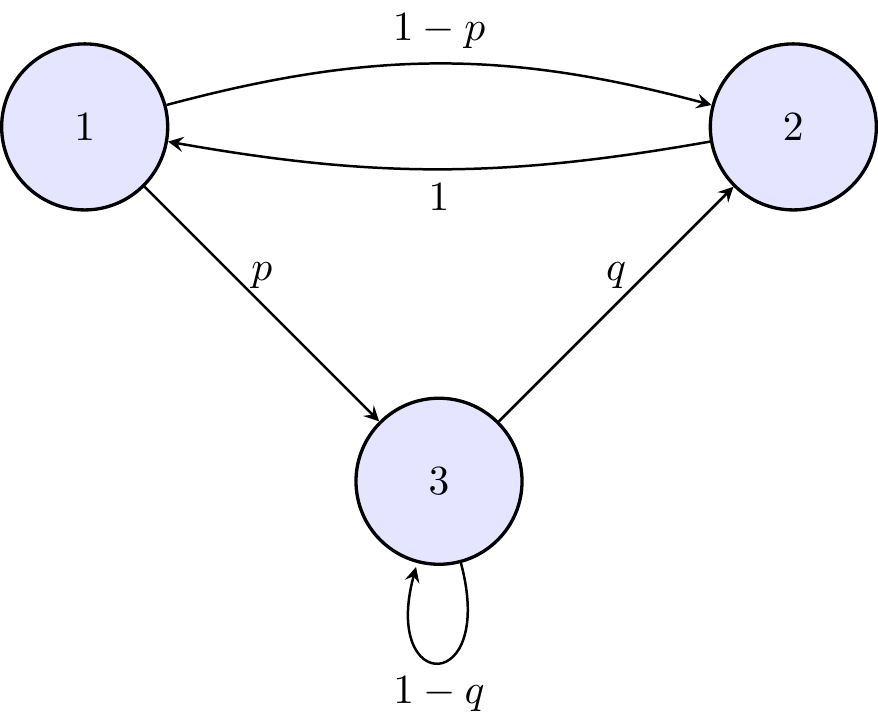
\includegraphics[width=0.4\linewidth]{index_files/figure-latex/Ex2.1ExerAlfredo-1} \end{center}

\begin{enumerate}
\def\labelenumi{(\alph{enumi})}
\item
  Determine a matriz das probabilidades de transição.
\item
  Em que condições esta cadeia é irredutível e aperiódica?
\item
  Determine a distribuição estacionária \(\pi=(\pi _{1},\pi _{2},\pi _{3})\).
\item
  Calcule os valores de \(p\) e \(q\) tais que \(\pi _{1}=\pi _{2}=\pi _{3}\).
\end{enumerate}

\end{exercise}

\(\,\)

\begin{exercise}
\leavevmode

Considere uma C.M. com espaço de estados \(E=\{1,2,3,4\}\) e matriz de transição
\[
\mathbb{P}=\left[
\begin{array}{cccc}
1/2 & 1/2 & 0 & 0 \\
1 & 0 & 0 & 0 \\
0 & 1/3 & 2/3 & 0 \\
1/2 & 0 & 1/2 & 0%
\end{array}
\right]
\]
Classifique os estados.

\end{exercise}

\(\,\)

\begin{exercise}
\leavevmode

Considere uma C.M. homogénea \(\{X_{n}, ~ n\geq 0\}\), com espaço de estados \(E=\{1,2,3\}\) e matriz de probabilidades de transição a um passo:
\[
\mathbb{P}=\left[
\begin{array}{ccc}
p & 1-p & 0 \\
0 & 0 & 1 \\
0 & 1-q & q%
\end{array}
\right] ,\;\;\;0<p<1\;\;\;\mathrm{e}\;\;\;0<q<1.
\]

\begin{enumerate}
\def\labelenumi{(\alph{enumi})}
\item
  Classifique, justificando, cada um dos estados da cadeia.
\item
  Calcule o limite
  \[\lim\limits_{n \to \infty }P(X_{n}=3).\]
\end{enumerate}

\end{exercise}

\(\,\)

\begin{exercise}
\leavevmode

Uma urna contém 6 bolas, das quais 3 são encarnadas e 3 são verdes. São selecionadas ao acaso da urna 2 bolas simultaneamente. Se uma for verde e a outra for encarnada, então são postas de lado e são colocadas duas bolas azuis na urna. Se não for o caso, colocam-se de volta as bolas retiradas na urna. O processo repete-se até só haver bolas azuis na urna.

Seja \(X_{n}\) o número de bolas encarnadas na urna depois da tiragem \(n\).

\begin{enumerate}
\def\labelenumi{(\alph{enumi})}
\item
  Justifique que \(\{X_{n}\}\) é uma C.M homogénea. Defina o espaço de estados e construa a respetiva matriz das probabilidades de transição.
\item
  Classifique, justificando, os estados da cadeia.
\item
  Calcule a probabilidade de, a determinada altura, a urna apenas conter bolas azuis partindo de \(X_{0}=3\).
\end{enumerate}

\end{exercise}

\(\,\)

\begin{exercise}
\leavevmode

Considere uma C.M com estados 0 e 1, e matriz de transição
\[
\mathbb{P}=\left[
\begin{array}{cc}
a & 1-a \\
1-b & b%
\end{array}
\right] \, , \; 0<a,~ b<1.
\]

\begin{enumerate}
\def\labelenumi{(\alph{enumi})}
\item
  Calcule a probabilidade do primeiro retorno ao estado 1 em \(n\) passos,
  \(f_{11}^{n}, ~n=1,2,...\), e verifique que o estado 1 é recorrente
  positivo.
\item
  Calcule a distribuição limite \((\pi _{0},\pi _{1})\) e discuta a
  sua existência. Relacione \(\pi _{1}\) com a média do tempo de
  primeiro retorno ao estado 1.
\end{enumerate}

\end{exercise}

\(\,\)

\begin{exercise}
\leavevmode

Considere a C.M \((X_{n}, ~n=0,1,\cdots )\) com espaço de estados \(E=\{0,1\}\) e tal que,
\[
0<p_{00}<1\;\;\;\mathrm{e}\;\;\;0<p_{11}<1.
\]

\begin{enumerate}
\def\labelenumi{(\alph{enumi})}
\item
  Prove que a cadeia é recorrente positiva.
\item
  Determine a distribuição estacionária da cadeia.
\end{enumerate}

\end{exercise}

\(\,\)

\begin{exercise}
\leavevmode

Considere uma C.M com espaço de
estados \(E=\{1,2,3,4\}\) e matriz de transição
\[
\mathbb{P}=\left[
\begin{array}{cccc}
1/3 & 2/3 & 0 & 0 \\
1/2 & 1/2 & 0 & 0 \\
1/4 & 0 & 1/4 & 1/2 \\
0 & 0 & 0 & 1%
\end{array}
\right]
\]

\begin{enumerate}
\def\labelenumi{(\alph{enumi})}
\item
  Classifique, justificando, os estados da cadeia.
\item
  Calcule \(f_{34}(n)\), a probabilidade de a primeira
  visita ao estado 4 ter lugar no \(n\)-ésimo passo, partindo de 3, e
  calcule a probabilidade de absorção no estado 4, partindo de 3.
\end{enumerate}

\end{exercise}

\(\,\)

\begin{exercise}
\leavevmode

Considere uma C.M. definida pela matriz das probabilidades
de transição:
\[
\mathbb{P}=\left[
\begin{array}{ccc}
0 & 2/3 & 1/3 \\
3/8 & 1/8 & 1/2 \\
1/2 & 1/2 & 0%
\end{array}
\right]
\]

\begin{enumerate}
\def\labelenumi{(\alph{enumi})}
\item
  Verifique que a cadeia é irredutível e aperiódica.
\item
  Verifique a existência de distribuição limite e determine-a.
\end{enumerate}

\end{exercise}

\(\,\)

\begin{exercise}
\leavevmode

Considere uma C.M. \((X_{n}, ~n=0,1,\dots)\) com espaço de estados \(E=\{1,2\}\), em que \(P_{12}=P_{21}=1\) e \(P(X_{0}=1)=P(X_{0}=2)=1/2\).

\begin{enumerate}
\def\labelenumi{(\alph{enumi})}
\item
  O que pode concluir quanto à convergência de \(P_{ii}^{n}, ~i=1,2\), quando \(n \to +\infty?\) Justifique.
\item
  Mostre que
  \[
  P(X_{n}=1)=P(X_{n}=2)=1/2,\;\;\;\forall \,n=1,2,\dots,
  \]
  isto é, a distribuição de \(X_{n}\) é estacionária. Comente e
  relacione justificadamente com a conclusão obtida na alínea
  anterior.
\end{enumerate}

\end{exercise}

\chapter{Cadeias de Markov em tempo contínuo}\label{cadeias-de-markov-em-tempo-continuo}

Neste capítulo iremos considerar \((X_t, ~ t \in \mathbb{R}_0^+)\) uma C.M. com valores em \(\mathbb{N}_0\) e espaço de parâmetro \(\mathbb{R}_0^+\).

Vamos admitir que \((X_t, ~ t \in \mathbb{R}_0^+)\) é homogénea, isto é, tem probabilidade de transição estacionárias. Nestas condições, a função de probabilidade de transição

\[\forall ~t >0, ~P_{ij}(t)=P(X_{t+n}=j \mid X_n=i), \quad i,j \in \mathbb{N}_0\]
é independente de \(n \geq 0\).

\section{Processo de Poisson homogéneo}\label{processo-de-poisson-homogeneo}

O processo de Poisson homogéneo é um processo estocástico que modela a ocorrência de eventos aleatórios ao longo do tempo, onde os eventos ocorrem de forma independente e com uma taxa constante. É frequentemente utilizado para modelar fenómenos como chamadas telefónicas recebidas num call center, chegadas de clientes a um serviço, ou falhas em sistemas, entre outros.

Seja \(X_t\) uma função que conta o número de vezes que um determinado acontecimento ocorre durante o período de tempo de 0 a \(t\). Assim, a aplicação \(t \longrightarrow X_t\) é uma função em escada, não decrescente, em que os saltos correspondem às ocorrências dos acontecimentos:

\begin{center}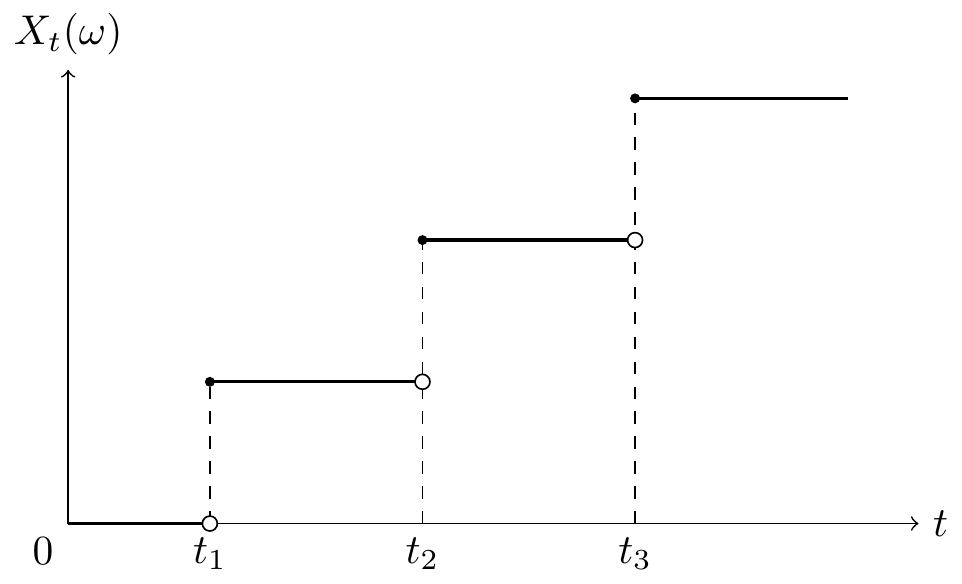
\includegraphics[width=0.5\linewidth]{index_files/figure-latex/fig6-1} \end{center}

\(\,\)

\begin{hypothesis}[Postulados do processo de Poisson]
\leavevmode

\begin{itemize}
\item
  P1. O número de acontecimentos que ocorrem em intervalos de tempo disjuntos são v.a.'s independentes.
\item
  P2. A v.a. \(X_{t_0+t}-X_{t_0}\) (isto é, o acréscimo) depende apenas de \(t\) e não de \(t_0\) ou de \(X_{t_0}\).
\item
  P3. A probabilidade de ocorrer pelo menos um acontecimento num intervalo de tempo pequeno de amplitude \(h\) é proporcional à amplitude desse intervalo. Assim,
  \[P(h)=\lambda h + o(h), \quad h \to 0, ~\lambda >0,\]
  onde \(g(t)=o(t), ~t \to 0, \iff \lim\limits_{t \to 0}\dfrac{g(t)}{t}=0.\)
\item
  P4. A probabilidade de ocorrer mais do que um acontecimento num intervalo de tempo pequeno de amplitude \(h\) é negligível quando \(h\) é pequeno. Isto mostra que num intervalo pequeno, ou ocorre um acontecimento, ou não ocorre nenhum, excluindo a possibilidade de ocorrência simultânea de dois ou mais acontecimentos. Assim,
  \[\sum\limits_{i=2}^{+\infty}P_i(k)=o(h), \quad h \to 0,\]
  onde \(P_i(k)=P(X_k=i)\).
\end{itemize}

\end{hypothesis}

\(\,\)

Representemos por \(P_n(t)\) a probabilidade de ocorrerem \(n\) acontecimentos no intervalo de tempo \([0,t]\). Assim, num intervlao de amplitude \(t+h\) temos:

\begin{itemize}
\tightlist
\item
  Para \(n=0\):
  \begin{align*}
  P_0(t+h) &= P_0(t) \cdot P_{0}(h)\\
         &= P_0(t) \cdot (1- P(\text{ocorrer mais do que 1 acontecimento}))\\
         &= P_0(t) \cdot (1-P(h))\\
         &= P_0(t) - P_0(t) \cdot P(h).
  \end{align*}
\end{itemize}

Temos então que:

\[P_0(t+h) -P_0(t) = - P_0(t) \cdot P(h) \iff \dfrac{P_0(t+h) -P_0(t)}{h} = - P_0(t) \cdot \dfrac{P(h)}{h}.\]
Aplicando limites, e tendo em conta o Postulado P3, obtemos:

\[\lim\limits_{h \to 0}\dfrac{P_0(t+h) -P_0(t)}{h} = - P_0(t) \cdot \lim\limits_{h \to 0} \dfrac{P(h)}{h},\]
o que resulta em

\[\dfrac{d}{dt}P_0(t) = - P_0(t) \cdot \lim\limits_{h \to 0} \dfrac{\lambda h + o(h)}{h},\]
ou seja,
\[\dfrac{d}{dt}P_0(t) = - \lambda P_0(t),\]
isto é, a probabilidade do acontecimento não se realizar no intervalo de tempo \([0,t]\), \(P_0(t)\), satisfaz a equação diferencial
\[\boxed{P^{'}_0(t)=-\lambda P_0(t).}\]

multiplicando pelo fator integrante \(e^{\lambda t}\), a solução desta equação diferencial é,
\[P_0(t)=K \cdot e^{-\lambda t},\]
onde \(K\) é uma constante de integração. Como \(P_0(0)=1\), temos que \(K=1\). Assim, a solução da equação diferencial é

\[\boxed{P_0(t)=e^{-\lambda t}.}\]

\begin{itemize}
\tightlist
\item
  Para \(n \geq 1\): se no intervalo \([0,t]\) ocorrerm \(n\) eventos, no intervalo \([t,t+h]\) ocorrem zero; se no intervalo \([0,t]\) ocorrerm \(n-1\) eventos, no intervalo \([t,t+h]\) ocorre 1; se no intervalo \([0,t]\) ocorrerm \(n-2\) eventos, no intervalo \([t,t+h]\) ocorrem 2; e assim sucessivamente. Logo,
\end{itemize}

\begin{align*}
P_n(t+h) &= P_n(t) \cdot P_{0}(h) + P_{n-1}(t) \cdot P_{1}(h) + P_{n-2}(t) \cdot P_{2}(h) + \dots\\
         &= P_n(t) \cdot P_{0}(h) + P_{n-1}(t) \cdot P_{1}(h) + \sum\limits_{i \geq 2}P_{n-i}(t) \cdot P_{i}(h)\\
         &= P_n(t) \cdot (1-P(h)) + P_{n-1}(t) \cdot (P(h)+o(h)) + \sum\limits_{i \geq 2}P_{n-i}(t) \cdot P_{i}(h),
\end{align*}
donde se obtém:
\[P_n(t+h)-P_n(t)=-P_n(t) \cdot P(h) + P_{n-1}(t) \cdot P(h) + P_{n-1}(t) \cdot o(h) + o(h)+\sum\limits_{i \geq 2}P_{n-i}(t) \cdot P_{i}(h).\]
Dividindo por \(h\) e aplicando o limite quando \(h \to 0\), obtemos:

\begin{align*}
\lim\limits_{h \to 0}\dfrac{P_n(t+h)-P_n(t)}{h} &= -P_n(t) \cdot \lim\limits_{h \to 0} \dfrac{P(h)}{h} + P_{n-1}(t) \cdot \lim\limits_{h \to 0} \dfrac{P(h)}{h} + P_{n-1}(t) \cdot \lim\limits_{h \to 0} \dfrac{o(h)}{h} \\
& + \lim\limits_{h \to 0} \dfrac{o(h)}{h}+\lim\limits_{h \to 0} \dfrac{\sum\limits_{i \geq 2}P_{n-i}(t) \cdot P_{i}(h)}{h},
\end{align*}
ou seja,
\[\dfrac{d}{dt}P_n(t)=-P_n(t) \cdot \lambda +  P_{n-1}(t) \cdot \lambda + 0 + 0,\]
o que equivale a escrever que a probabilidade do acontecimento se realizar pelo menos uma vez no intervalo \([0,t]\) satisfaz a equação diferencial
\[\boxed{P^{'}_n(t)=\lambda P_{n-1}(t) - \lambda P_n(t), \quad n \in \mathbb{N}.}\]
A solução desta equação diferencial, tendo em conta que \(P_n(0)=0\), é dada por

\[\boxed{P_n(t)=\dfrac{\lambda^n t^n}{n!} e^{-\lambda t}, \quad n \in \mathbb{N}.}\]

Assim, podemos concluir que a probabilidade de ocorrerem \(n\) acontecimentos no intervalo de tempo \([0,t]\) segue uma distribuição de Poisson com parâmetro \(\lambda t\), ou seja,

\[X_t \sim Po(\lambda t),\]
donde
\[
P(X_t=n)=P_n(t)=\dfrac{(\lambda t)^n}{n!} e^{-\lambda t}, \quad n \in \mathbb{N}_0.
\]

Das propriedades da distribuição de Poisson, sabemos que \(E(X_t)=\lambda t\), o que significa que o número esperado de acontecimenrtos num intervalo de amplitude \(t\) é proporcional à amplitude do intervalo.

No caso \(t=1\), temos que \(E(X_1)=\lambda\), pelo que:

\begin{itemize}
\item
  \(\lambda\) representa o número médio de acontecimentos que ocorrem por unidade de tempo;
\item
  \(\lambda\) designa a taxa de ocorrência, razão ou intensidade do processo de Poisson homogéneo.
\end{itemize}

Com base no exposto, podemos definir processo de Poisson homogéneo do seguinte modo:

\begin{definition}[Processo de Poisson homogéneo]

Um processo estocástico \((X_t, ~ t \in \mathbb{R}_0^+)\) é um \textbf{processo de Poisson homogéneo} com taxa \(\lambda >0\) sse:

\begin{enumerate}
\def\labelenumi{(\roman{enumi})}
\item
  tem incrementos independentes e estacionários, e \(X_0=0\) q.c. (quase certamente);
\item
  \(X_t\) segue uma distribuição de Poisson com parâmetro \(\lambda t\), isto é, \(X_t \sim Po(\lambda t)\), para todo \(t \in \mathbb{R}_0^+\).
\end{enumerate}

\end{definition}

\(\,\)

\begin{remark}[Observações sobre o processo de Poisson homogéneo]
\leavevmode

\begin{enumerate}
\def\labelenumi{\arabic{enumi}.}
\tightlist
\item
  Os postulados do processo de Poisson são suficientes para defini-lo e permitem também definir completamente a distribuição do vetor \((X_{t_1},X_{t_2},\dots, X_{t_k})\). Com efeito,
  por um lado verifica-se
  \[\forall ~s,t \in \mathbb{R}_0^+: 0 \leq s \leq t, ~X_t-X_s \sim Po(\lambda(t-s)),\]
  isto é, o número de acontecimentos que ocorrem num certo intervalo só depende da amplitude desse intervalo:
  \begin{align*}
  X_t-X_s & ~ {\buildrel d \over =} ~ X_{t-s+s}-X_s\\
       & ~ {\buildrel d \over =} ~  X_{t-s}-X_0\\
       & ~ {\buildrel d \over =} ~  X_{t-s}\\
       & = ~ Po(\lambda(t-s)).
  \end{align*}
  Por outro lado, como os incrementos são independentes, temos que, para \(t_1 < t_2 < \dots < t_k\):
\end{enumerate}

\begin{align*}
P(X_{t_1}=n_1, \dots, X_{t_k}=n_k) & =  P(X_{t_1}=n_1, \dots, X_{t_k}-X_{k_1}=n_k-n_{k-1})\\
        & =  P(X_{t_1}=n_1) \cdots P(X_{t_k}-X_{t_{k-1}}=n_k-n_{k-1})\\
        & =  \dfrac{(\lambda t_1)^{n_1}}{n_1!} e^{-\lambda t_1} \cdots \dfrac{(\lambda(t_k-t_{k-1}))^{n_k-n_{k-1}}}{(n_k-n_{k-1})!} e^{-\lambda(t_k-t_{k-1})}.
\end{align*}

\begin{enumerate}
\def\labelenumi{\arabic{enumi}.}
\setcounter{enumi}{1}
\tightlist
\item
  Ligada à v.a. \(X_t\) costuma definir-se ainda a v.a. \(L\) que representa o tempo de espera até ao primeiro acontecimento, isto é, \(L=\inf\{t \in \mathbb{R}_0^+: X_t>0\}\). A v.a. \(L\) segue uma distribuição exponencial com parâmetro \(\lambda\), ou seja, \(L \sim Exp(\lambda)\). Vejamos:
\end{enumerate}

\begin{itemize}
\tightlist
\item
  \(F_L(t)=P(L \leq t)=1-P(L>t)=1-P(X_t=0)=1-P_0(t)=1-e^{-\lambda t}\).
\item
  \(f_L(t)=\lambda e^{-\lambda t}, \quad t>0.\)
\item
  \(E(L)=1/\lambda\).
\item
  \(Var(L)=1/\lambda^2\).
\item
  \(M_L(t)=\dfrac{\lambda}{\lambda-t}, ~t< \lambda\). (f.g.m.).
\end{itemize}

\begin{enumerate}
\def\labelenumi{\arabic{enumi}.}
\setcounter{enumi}{2}
\item
  Considere-se a seguinte v.a.:
  \[S_r=\text{ tempo de espera até à ocorrência do } r\text{-ésimo acontecimento},\]
  isto é,
  \[S_r=X_1+X_2+\dots+X_r, \quad X_i \text{ i.i.d.},\]
  onde \(X_i\) representa o tempo de espera desde o \((i-1)-\)ésimo acontecimento até ocorrer o acontecimento de ordem \(i\). Assim,
  \(X_i \sim Exp(\lambda), ~\forall ~i =1, \dots,r.\) Assim, calculando a f.g.m. de \(S_r\), e relacionando com a f.g.m. de \(X_i\) vem:
  \[
  M_{S_r}(t)=\prod\limits_{i=1}^{r}M_{X_i}(t)=(M_{X_i}(t))^r=\left(\dfrac{\lambda}{\lambda-t}\right)^r, ~t< \lambda,
  \]
  ou seja, trata-se da f.g.m. de uma v.a. com distribuição Gamma com parâmetros \(r\) e \(\lambda\), ou seja, \(S_r \sim \Gamma(r,\lambda)\), donde se obtém,
  \[E(S_r)=r/\lambda \quad { e } \quad Var(S_r)=r/\lambda^2.\]
\item
  O processo de Poisson é uma cadeia de Markov em tempo contínuo homogénea, isto é, \(\forall ~k_1,k_2,\dots,k_n,k \in \mathbb{N}_0, ~\forall ~t_1,t_2,\dots,t_n \in \mathbb{R}_0^+, ~t_1 \leq t_2 \leq \dots \leq t_n \leq t\):
  \[P(X_{t}=k \mid X_{t_1}=k_1, \dots,X_{t_n}=k_n)=P(X_t=k \mid X_{t_n}=k_n)=P_{k_nk}(t-t_n).\]
\end{enumerate}

\end{remark}

Pelo exposto, podemos dar uma outra definição de processo de Poisson:

\begin{definition}[Processo de Poisson homogéneo]

Se \((X_t, ~ t \in \mathbb{R}_0^+)\) é um \textbf{processo de Poisson homogéneo} com taxa \(\lambda >0\), então \((X_t, ~ t \in \mathbb{R}_0^+)\) é uma cadeia de Markov com valores em \(\mathbb{N}_0\), tal que:

\begin{enumerate}
\def\labelenumi{(\roman{enumi})}
\item
  \(P(X_{t+h}-X_t=1 \mid X_{t}=x)=\lambda h + o(h), ~x \in \mathbb{N}_0\), quando \(h \to 0\).
\item
  \(P(X_{t+h}-X_t=0 \mid X_{t}=x)=1-\lambda h + o(h), ~x \in \mathbb{N}_0\), quando \(h \to 0\).
\item
  \(X_0=0\) q.c.
\end{enumerate}

\end{definition}

\(\,\)

Existem cadeias de Markov mais gerais e que nos permitem descrever fenómenos análogos aos descritos pelos processos de Poisson. É o que veremos nas secções seguintes.

\(\,\)

\begin{exercise}
\leavevmode

Seja \(X=(X_t: ~t \geq 0)\) um PE real tal que \(X_0=0\) q.c. e \(X_t \sim Po(\cdot)\).

\begin{enumerate}
\def\labelenumi{(\alph{enumi})}
\item
  Em que condições será \(X\) um processo de Poisson?
\item
  Supondo que \(X\) é um processo de Poisson, prove que \(\forall ~t,s,h \in \mathbb{R}_0^+\), com \(t>s>h\), e \(\forall ~x,y \in \mathbb{N}_0\):
  \[P(X_t-X_s=x, X_s-X_h=y)=\dfrac{e^{-\lambda (t-h)} \lambda^{x+y} (t-s)^x (s-h)^y}{x!y!}.\]
\end{enumerate}

\end{exercise}

\(\,\)

\begin{exercise}
\leavevmode

Considere uma estação de serviço de lavagem de automóveis na qual apenas um carro é atendido de cada vez e segundo a ordem de chegada. Um estudo realizado pela empresa permitiu concluir que as chegadas dos automóveis ocorrem segundo um processo de Poisson com intensidade média de 15 carros por hora. Designe por \(N_t,~t \geq 0\), o número de automóveis que chegam num intervalo de tempo de amplitude \(t\) minutos.

\begin{enumerate}
\def\labelenumi{(\alph{enumi})}
\item
  Identifique a distribuição de \(N_t, ~ \forall ~t \geq 0\). Justifique a sua resposta.
\item
  Mostre que
  \[\lim\limits_{h \to 0} \dfrac{P(N_h \geq 2)}{P(N_h =1)}=0.\]
\end{enumerate}

\begin{enumerate}
\def\labelenumi{\alph{enumi})}
\setcounter{enumi}{2}
\item
  Prove que a condição expressa na alínea anterior é equivalente a
  \[\lim\limits_{h \to 0} P(N_h >1 \mid N_h \geq 1 )=0.\]
  O que pode concluir sobre o processo em causa?
\item
  Qual o tempo médio de espera entre duas chegadas consecutivas?
\end{enumerate}

\end{exercise}

\(\,\)

\begin{exercise}
\leavevmode

Seja \((N_t, ~ t \geq 0)\) um processo de Poisson de intensidade \(\lambda >0\).

\begin{enumerate}
\def\labelenumi{(\alph{enumi})}
\tightlist
\item
  Supondo que \(s<t\), calcule:
\end{enumerate}

\begin{enumerate}
\def\labelenumi{\roman{enumi}.}
\item
  \(E(N_t-N_s)\).
\item
  \(Var(N_t-N_s)\).
\item
  \(Cov(N_t,N_s)\).
\end{enumerate}

\begin{enumerate}
\def\labelenumi{(\alph{enumi})}
\setcounter{enumi}{1}
\tightlist
\item
  Os Clientes de um vendedor de jornais chegam segundo um processo de Poisson a uma velocidade média de 2 Clientes por minuto.
\end{enumerate}

\begin{enumerate}
\def\labelenumi{\roman{enumi}.}
\item
  Determine a probabilidade de não chegarem Clientes nos próximos três minutos sabendo que chegaram um ou mais Clientes nos últimos cinco minutos.
\item
  O vendedor costuma fazer a seguinte aposta: paga ao seu assistente um euro se o próximo Cliente não chegar dentro de um minuto, caso contrário o assitente paga-lhe um euro. Qual o valor que o vendedor espera ganhar?
\end{enumerate}

\end{exercise}

\(\,\)

\begin{exercise}
\leavevmode

O volume de vendas de um determinado produto constitui um processo de Poisson, com um volume médio de vendas de 4 unidades por dia.

\begin{enumerate}
\def\labelenumi{(\alph{enumi})}
\item
  Qual é a probabilidade de que, em dois dias, se vendam exatamente 6 unidades?
\item
  Qual é a probabilidade de que, em dois dias, se vendam mais de 6 unidades?
\item
  Determine o volume médio de vendas semanal.
\item
  Qual é a probabilidade de que um stock de 4 unidades dure menos de um dia?
\end{enumerate}

\end{exercise}

\(\,\)

\begin{exercise}
\leavevmode

Numa loja os clientes chegam de acordo com uma lei de Poisson à média de 30 por hora. Qual a probabilidade de que o intervalo de tempo
entre chegadas sucessivas seja:

\begin{enumerate}
\def\labelenumi{(\alph{enumi})}
\item
  Superior a 2 minutos?
\item
  Inferior a 4 minutos?
\item
  Entre 1 e 3 minutos?
\end{enumerate}

\end{exercise}

\(\,\)

\begin{exercise}
\leavevmode

Uma v.a. \(T\) diz-se \emph{sem memória} sse:
\[
P(T>x+y \mid T>x)=P(T>y),\;\;\;\forall \;x,y>0.
\]
Mostre que:

\begin{enumerate}
\def\labelenumi{(\alph{enumi})}
\item
  Se \(T\) for uma v.a. contínua, \(T\) é sem memória sse \(T\) for distribuída exponencialmente.
\item
  Se \(T\) tomar apenas valores inteiros e positivos, \(T\) é sem memória para \(x\) e \(y\) não negativos sse existe uma constante \(p\) tal
  que:
  \[
  P(T=k)=p(1-p)^{k-1},\;\;\;k=1,2,3,\cdots .
  \]
\end{enumerate}

\end{exercise}

\(\,\)

\begin{exercise}
\leavevmode

A chegada de passageiros a uma paragem de autocarro segue um processo de Poisson com intensidade \(\lambda\). Suponha que um autocarro partiu no instante \(t=0\), não tendo deixado nenhum passageiro em espera. Seja \(T\) o tempo de chegada do autocarro seguinte. Então, o número de pessoas na paragem aquando da sua chegada é \(N(T)\). Suponha que o tempo de chegada \(T\) é independente do processo de Poisson e que \(T\) tem distribuição uniforme no intervalo \((1,2)\).

Calcule a média e a variância de \(N(T)\).

\end{exercise}

\(\,\)

\begin{exercise}
\leavevmode

Sejam \((N_t, ~t\geq 0)\) um processo de Poisson com intensidade \(\lambda\) e \(P_{k}(t)=P(N_t=k), ~k=0,1,2,\dots\).

\begin{enumerate}
\def\labelenumi{(\alph{enumi})}
\item
  Deduza as equações diferenciais:
  \begin{eqnarray*}
  P_{0}^{\prime }(t) &=&-\lambda P_{0}(t) \\
  P_{k}^{\prime }(t) &=&-\lambda P_{k}(t)+\lambda P_{k-1}(t)\, ,%
  ~ k=1,2,\cdots
  \end{eqnarray*}
\item
  Encontre a partir das equações acima a função de
  probabilidade:
  \[
  P_{k}(t)=\frac{(\lambda t)^{k}}{k!}e^{-\lambda t} , \,k=0,1,2,\dots
  \]
\end{enumerate}

\end{exercise}

\section{Processo de nascimento puro}\label{processo-de-nascimento-puro}

Considere-se uma sucessão de números positivos \(\{\lambda_k, ~k \in \mathbb{N}_0\}\).

\begin{definition}[Processo de nascimento puro]

Um processo estocástico \((X_t, ~ t \in \mathbb{R}_0^+)\), com valores em \(\mathbb{N}_0\), é um \textbf{processo de nascimento puro} com taxa (ou razão de nascimento) \(\{\lambda_k, ~k \in \mathbb{N}_0\}\) se é uma cadeia de markov em tempo contínuo homogénena, satisfazendo os axiomas:

\begin{enumerate}
\def\labelenumi{(\roman{enumi})}
\item
  \(P(X_{t+h}-X_t=1 \mid X_{t}=k)=\lambda_k h + o_{1,k}(h)=P_{k,k+1}(h)\).
\item
  \(P(X_{t+h}-X_t=0 \mid X_{t}=k)=1-\lambda_k h + o_{2,k}(h)=P_{k,k}(h)\).
\item
  \(P(X_{t+h}-X_t < 0 \mid X_{t}=k)=0, ~ k \in \mathbb{N}_0\), quando \(h \to 0\).
\item
  \(X_0=0\) q.c.
\end{enumerate}

\end{definition}

\(\,\)

\begin{remark}
\leavevmode

\begin{enumerate}
\def\labelenumi{\arabic{enumi}.}
\item
  A condição (iv) é admita por conveniência.
\item
  \(X_t\) \textbf{não} representa o tamanho da população mas o número de nascimentos no intervalo \([0,t]\).
\item
  Uma vez que as probabilidades de transição dadas por (i) e (ii) são estacionárias, então \(o_{1,k}(h)\) e \(o_{2,k}(h)\) não dependem de \(t\).
\item
  O processo de nascimento puro é uma generalização do processo de Poisson homogéneo, onde a probabilidade de um acontecimento ocorrer num certo instante depende do número de acontecimentos que já ocorreram. Assim, o processo de Poisson é um processo de nascimento puro de rezão de nascimento constante e igual \(\lambda\).
\end{enumerate}

\end{remark}

\(\,\)

Considere-se agora
\[P_n(t)=P(X_t=n),\]
e atente-se ao Teorema seguinte:

\begin{theorem}
\(P_n(t)\) satisfaz, para \(t \geq 0\), o sistema de equações diferenciais
\[
\begin{cases}
P^{\prime}_0(t)=-\lambda_0 P_0(t), \\
P^{\prime}_n(t)=\lambda_{n-1} P_{n-1}(t) - \lambda_n P_n(t), ~ n \geq 1
\end{cases},
\]
com as condições fronteira
\[
\begin{cases}
P_0(0)=P(X_0=0)=1, \\
P_n(0)=P(X_0=n)=0, ~ n >0.\\
\end{cases}
\]
Adicionalmente,

\[P_0(t)=P(X_t=0)=e^{\lambda_0 t}.\]
\end{theorem}

\(\,\)

Consideremos agora a v.a.
\[T_k= \text{ tempo compreendido entre o instante } k \text{ e o } k+1-\text{ésimo nascimentos consecutivos},\]
isto é
\[T_k= \text{ tempo de espera entre nascimentos consecutivos}.\]

Tem-se que
\[P_n(t)=P(X_t=n)=P\left(\sum\limits_{i=0}^{n-1}T_i \leq t \leq \sum\limits_{i=0}^{n}T_i\right).\]
Considere-se
\[S_k=\sum\limits_{i=0}^{k-1}T_i,\]
o tempo durante o qual ocorrem \(k\) nascimentos. Como se viu anteriormente,
\[\forall z >0, ~P(T_0 \leq z)= 1-P(X_z=0)=1-e^{-\lambda_0 z},\]
isto é,
\[T_0 \sim Exp(\lambda_0).\]

É possivel provar (ver Karlin \& Taylor, por exemplo) que \((T_k, ~ k \in \mathbb{N}_0)\) é uma sucessão de v.a.'s independentes, tais que, para cada \(k \in \mathbb{N}_0\), \(T_k \sim Exp(\lambda_k)\).

Adicionalmente, se \((X_t, t \geq 0)\) é um processo de Poisson, então \(S_n\) segue uma distribuição Gamma com parâmetros \(n\) e \(\lambda\), ou seja, \(S_n \sim \Gamma(n,\lambda)\), onde \(\lambda\) é a taxa do processo de Poisson.

Terminamos esta secção com o seguinte Teorema:

\begin{theorem}
\(P_k(t)\) verifica a equação de recorrência
\[P_k(t)=\lambda_{k-1} e^{-\lambda_k t}\int\limits_{0}^{1}e^{\lambda_k x}P_{k-1}(x) \, dx, \quad k \in \mathbb{N}.\]
\end{theorem}

\(\,\)

\begin{exercise}
\leavevmode

Com vista ao bom funcionamento de determinado consultório médico, a direção determinou que em cada instante, do período de funcionamento do mesmo, não poderia existir no consultório mais do que \(N\) doentes. Apenas um doente é atendido de cada vez e segundo a respetiva ordem de chegada. Os doentes chegam ao consultório segundo um processo de Poisson de intensidade \(1/2\), ficando a aguardar a sua vez de atendimento apenas se nesse momento o número de utentes no consultório for inferior a \(N\). As consultas são concluídas segundo um processo de Poisson de intensidade \(1/3\).

\begin{enumerate}
\def\labelenumi{(\alph{enumi})}
\tightlist
\item
  Designe por \(N_t, ~t \geq 0\), o número de doentes que chegam num intervalo de amplitude \(t\).
\end{enumerate}

\begin{enumerate}
\def\labelenumi{\arabic{enumi}.}
\item
  Prove que:

  \begin{enumerate}
  \def\labelenumii{\roman{enumii}.}
  \item
    \((N_t, ~t \geq 0)\) é uma C.M. de tempo contínuo homogénea e indica a respetiva probabilidade de transição.
  \item
    \((N_t, ~t \geq 0)\) é um processo de nascimento puro.
  \end{enumerate}
\item
  Sendo \(T\) uma v.a. que representa o tempo de espera entre duas chegadas consecutivas, prove que
  \[P(T > t)=e^{-t/2}, \quad t > 0.\]
\item
  Qual o tempo médio de espera entre chegadas?
\end{enumerate}

\begin{enumerate}
\def\labelenumi{(\alph{enumi})}
\setcounter{enumi}{1}
\tightlist
\item
  Seja agora \(X_t, ~t \geq 0\), o número total de doentes no consultório no instante \(t\) Supondo que:
  \[\forall ~k \in \{0,1,2,\dots,N\}: ~P(X_t=k)=\big(\dfrac{3}{2}\big)^k P(X_t=0),\]
  determine:
\end{enumerate}

\begin{enumerate}
\def\labelenumi{\arabic{enumi}.}
\item
  a probabilidade de que existam \(k\) doentes à espera de serem atendidos, num qualquer instante \(t\).
\item
  o número médio de doentes no consultório, num qualquer instante \(t\).
\end{enumerate}

\end{exercise}

\(\,\)

\begin{exercise}
\leavevmode

Considere um quiosque no qual os Clientes chegam de acordo com um processo de Poisson à razão de 32 Clientes por dia, durante o horário diário de abertura do quiosque (o qual corresponde a 8 horas). Designe por \(N_t, ~t \geq 0\), o número de Clientes que chegam ao quiosque num intervalo de tempo de amplitude \(t\) horas.

\begin{enumerate}
\def\labelenumi{\alph{enumi})}
\item
  Identifique, justificando, a distribuição de \(N_t\).
\item
  Sendo \(T_2\) a v.a. que representa o instante de chegada (em horas) do segundo Cliente ao quiosque, em cada dia, mostre que:
  \[P(T_2>t)=e^{-4t}(1+4t), \quad t>0.\]
\end{enumerate}

\end{exercise}

\(\,\)

\begin{exercise}
\leavevmode

Uma população de organismos evolui da forma seguinte: cada organismo existe independentemente dos outros, e vive durante determinado tempo, aleatório, com distribuição exponencial de parâmetro \(\theta\), dividindo-se então em dois novos organismos. Por sua vez, a sua existência é também independente dos outros organismos e têm um tempo de vida exponencialmente distribuído de parâmetro \(\theta\), e assim sucessivamente.

Seja \(X(t)\) o número de organismos existentes no instante \(t\). Suponha que \(X(0) = 1\) e defina \(P_n(t) = P(X(t) = n)\). Justifique que \(X(t)\) é um processo de nascimento puro, ou seja, verifica
\[
P_n'(t) = -\theta \left( n\,P_n(t) - (n-1)\,P_{n-1}(t) \right), \quad n = 1,2,\ldots
\]

\end{exercise}

\(\,\)

\begin{exercise}
\leavevmode

Considere uma população de dimensão \(N(t)\) no instante \(t\) tal que \(N(0) = 1\). Admita que qualquer dos membros desta população se divide em dois novos membros no intervalo \([t, t+h]\) com probabilidade \(\lambda h + o(h)\) ou mantém-se inalterado neste intervalo com probabilidade \(1 - \lambda h + o(h)\).

\begin{enumerate}
\def\labelenumi{(\alph{enumi})}
\item
  Prove que \((N(t), ~ t \geq 0)\) é um processo de nascimento puro com taxa de natalidade \(\lambda_n = n \lambda\), para todo o \(n = 1, 2, \cdots\).
\item
  Designe por \(p_k(t) = P(N(t) = k)\), com \(k = 1, 2, \cdots\) e prove que:
  \[
  p_k'(t) = (k-1)\lambda\, p_{k-1}(t) - k\lambda\, p_k(t), \quad k = 1,2,\cdots.
  \]
\item
  Tendo em conta a equação diferencial anterior, conclua por indução que:
  \[
  p_k(t) = e^{-k\lambda t} \left( e^{\lambda t} - 1 \right)^{k-1}, \quad k = 1,2,\cdots.
  \]
\item
  Seja \(P(z,t) = \sum\limits_{k=1}^{\infty} z^k p_k(t)\) a função geradora das probabilidades \(p_k(t)\). Prove que:
  \[
  P(z,t) = \frac{z e^{-\lambda t}}{1 - z + z e^{-\lambda t}}.
  \]
\item
  Calcule \(E(N(t))\).
\end{enumerate}

\end{exercise}

\(\,\)

\begin{exercise}
\leavevmode

Seja \((N(t), ~t \geq 0)\) um processo de nascimento puro com \(N(0) = I\) e taxa de natalidade \(\lambda_n = n \lambda\), sendo \(I\) um inteiro positivo. Designe por \(P_n(t) = P(N(t) = n)\).

\begin{enumerate}
\def\labelenumi{(\alph{enumi})}
\item
  Prove que:
  \begin{align*}
    P_I'(t) &= -I\lambda\, P_I(t) \\
    P_n'(t) &= -n\lambda\, P_n(t) + (n-1)\lambda\, P_{n-1}(t), \quad n = I+1, I+2, \ldots
  \end{align*}
\item
  Prove que:
  \[
  P_k(t) = \binom{k-1}{I-1} e^{-I\lambda t} \left( 1 - e^{-\lambda t} \right)^{k - I}, \quad k \geq I.
  \]
\end{enumerate}

\end{exercise}

\section{Processo de nascimento e morte}\label{processo-de-nascimento-e-morte}

\subsection{Definição e equações de Chapman-Kolmogorov}\label{definicao-e-equacoes-de-chapman-kolmogorov}

\begin{definition}[Processo de nascimento e morte]
Um processo estocástico \((X_t, ~ t \in \mathbb{R}_0^+)\), com valores em \(\mathbb{N}_0\), é um \textbf{processo de nascimento e morte} com taxas \(\{\lambda_k, ~k \in \mathbb{N}_0\}\) e \(\{\mu_k, ~k \in \mathbb{N}_0\}\) se é uma cadeia de markov em tempo contínuo homogénea, satisfazendo os axiomas:

\begin{enumerate}
\def\labelenumi{\arabic{enumi}.}
\item
  \(P_{i,i+1}(h)=P(X_{t+h}=i+1 \mid X_{t}=i)=\lambda_i h + o(h), ~i \geq 0\),
\item
  \(P_{i,i-1}(h)=P(X_{t+h}=i-1 \mid X_{t}=i)=\mu_i h + o(h), ~i \geq 1\),
\item
  \(P_{i,i}(h)=P(X_{t+h}=i \mid X_{t}=i)=1-(\lambda_i+\mu_i) h + o(h), ~ i \geq 0\),
\item
  \(P_{i,j}(0)=P(X_{t}=j \mid X_{t}=i)=\delta_{ij}\),
\item
  \(\mu_0=0, ~\lambda_0 >0, ~\mu_i, ~\lambda_i>0, ~i \in \mathbb{N}\),
\end{enumerate}

onde \(o(h)\), em cada caso, pode depender de \(i\) e considera-se que \(o(h) \to 0\) quando \(h \to 0\).

Quando ocorre um nascimento o processo passa do estado \(E_k\) para o estado \(E_{k+1}\) e, quando ocorre uma morte, o processo passa do estado \(E_k\) para o estado \(E_{k-1}\). Assim, o processo de nascimento e morte é um processo de nascimento puro com a adição de mortes.
\end{definition}

\(\,\)

\begin{remark}
Uma das generalizações óbvias dos processos de nascimento puro considerados consiste em permitir que \(X_t\) decresça, por exemplo através da morte dos seus memebros. Assim, se no instante \(t=0\) o processo está no estado \(n\) ele poderá mudar-se para os estados vizinhos \(n+1\) ou \(n-1\) após um tempo de espera aleatório. Um processo de nascimento e morte pode assim ser interpretado como um passeio aleatório de tempo contínuo.
\end{remark}

\(\,\)

Num processo de nascimento e morte (com espaço de estados \(\mathbb{N}_0\)) observa-se, \(\forall ~t\in\mathbb{R}_0^+\) e \(\forall ~ i,j\in\mathbb{N}_0\):

\begin{enumerate}
\def\labelenumi{\arabic{enumi}.}
\item
  \(P_{ij}(t) \geq 0\), ou seja, as probabilidades de transição são não negativas para quaisquer pares \((i,j)\) e qualquer tempo \(t\). Note-se que, em particular, \(P_{ij}(0)=\delta_{ij}\), onde \(\delta_{ij}\) é o símbolo de Kronecker, i.e., \(\delta_{ij}=1\) se \(i=j\) e \(\delta_{ij}=0\) se \(i \neq j\);
\item
  \(\displaystyle \sum_{j=0}^{\infty} P_{ij}(t)=1\), ou seja, a soma das probabilidades de transição a partir do estado \(i\) para todos os estados possíveis é igual a 1, para qualquer tempo \(t\);
\item
  As probabilidades de transição são dadas por: \(\forall ~s,t, \in \mathbb{R}_0^+\),
  \begin{align*}
  P_{ij}(t+s) &= P(X_{n+t+s}=j \mid X_n=i)  \\
           &= \sum\limits_{k=0}^{+\infty} P(X_{n+t+s}=j, X_{n+t}=k \mid X_n=i) \\
           &= \sum\limits_{k=0}^{+\infty} P(X_{n+t+s}=j \mid X_{n+t}=k, X_n=i) \cdot P(X_{n+t}=k \mid X_n=i) \\
           &= \sum\limits_{k=0}^{+\infty} P(X_{n+t+s}=j \mid X_{n+t}=k) \cdot P(X_{n+t}=k \mid X_n=i) \\
           &= \sum\limits_{k=0}^{+\infty} P_{kj}(s) \cdot P_{ik}(t).
  \end{align*}
\end{enumerate}

Temos então as \textbf{Equações de Chapmnan-Kolmogorov}:
\begin{equation}
\label{eq:chapkol}
\boxed{P_{ij}(t+s)=\sum\limits_{k=0}^{+\infty} P_{kj}(s) P_{ik}(t).}
\end{equation}

Nesta dedução, em cada igualdade, utilizamos, respetivamente, as seguintes justificações:

\begin{enumerate}
\def\labelenumi{\arabic{enumi}.}
\item
  Definição da probabilidade de transição do estado \(i\) para o estado \(j\) em \(t+s\) passos, a partir do instante \(n\).
\item
  Aplicação da regra da probabilidade total, ao considerar todos os possíveis estados \(k\) em que a cadeia pode estar no instante intermédio \(n+t\).
\item
  Aplicação da regra do produto das probabilidades condicionadas.
\item
  Aplicação da propriedade de Markov, que garante que o futuro (a partir de \(n+t\)) depende apenas do estado atual \(X_{n+t}=k\), e não do passado \(X_n=i\).
\item
  Finalmente, identificamos as probabilidades de transição:
  \[P_{kj}(s) = P(X_{n+t+s}=j \mid X_{n+t}=k) \text{ e } P_{ik}(t) = P(X_{n+t}=k \mid X_n=i).\]
\end{enumerate}

\(\,\)

As probabilidades de transição e as leis marginais caracterizam a distribuição do processo. As distribuições marginais dependem apenas da distribuição inicial e das probabilidades de transição. Assim, se
\[q_i:=P(X_0=i), ~i \in \mathbb{N}_0,\]
tem-se, \(\forall ~n \in \mathbb{N}_0\),
\begin{align*}
P(X_t=n) &= \sum\limits_{i=0}^{+\infty} P(X_{t}=n, X_{0}=i) \\
         &= \sum\limits_{i=0}^{+\infty} P(X_{0}=i) \cdot P(X_{t}=n \mid X_{0}=i) \\
         &= \sum\limits_{k=0}^{+\infty} P_{in}(t) \cdot q_i. \\
\end{align*}
Assim, as distribuições marginais do processo de nascimento e morte são dadas por
\[\boxed{P(X_t=n)=\sum\limits_{i=0}^{+\infty} P_{in}(t) q_i, ~n \in \mathbb{N}_0.}\]

\subsection{Tempo de espera}\label{tempo-de-espera}

Considere-se agora a v.a.

\[T_i=\text{tempo de espera de } X_t \text{ no estado } i.\]

É possível mostrar (Karlin \& Taylor, por exemplo) que, quando \(h \to 0\),

\[P(T_i \geq t+h)=P(T_i \geq t) \cdot P(T_i \geq h).\]

Podemos ainda escrever a igualdade anterior do seguinte modo

\begin{align*}
P(T_i \geq t+h) &= P(T_i \geq t) \cdot P(T_i \geq h) \\
                &= P(T_i \geq t) \cdot P(X_{n+h}=i, X_{s+n}=i \mid X_n=i), \quad \forall ~s \in [0,h] \\
                &= P(T_i \geq t) \cdot (P_{ii}(h) + o(h))\\
                &= P(T_i \geq t) \cdot (1-(\lambda_i+\mu_i)h + o(h))\\
                &= P(T_i \geq t) \cdot (1-(\lambda_i+\mu_i))+ o(h).\\
\end{align*}

Designando por \(G_i(t)=P(T_i \geq t)\), obtemos

\[G_i(t+h)=G_i(t) \cdot (1-(\lambda_i+\mu_i)h) + o(h),\]

donde, dividindo por \(h\) e aplicando o limite quando \(h \to 0\), obtemos

\[\dfrac{d}{dt}G_i(t) = -(\lambda_i+\mu_i) G_i(t),\]

pelo que,

\[G_i(t) = \exp\{-(\lambda_i+\mu_i)t\} = 1-(1-\exp\{-(\lambda_i+\mu_i)t\}),\]

isto é,

\[P(T_i \geq t)=1-\exp\{-(\lambda_i+\mu_i)t\}, \quad t \geq 0,\]

ou seja,

\[\boxed{T_i \sim Exp(\lambda_i+\mu_i),}\]

e o tempo médio de espera é dado por

\[\dfrac{1}{\lambda_i+\mu_i}.\]

\(\,\)

\begin{remark}
A descrição do movimento de \(X_t\) descreve-se a seguir. O processo permanece num certo estado \(i\) por um tempo aleatótio \(T_i\) seguindo uma distribuição exponencial de parâmetro \(\lambda_i+\mu_i\). Quando deixa o estado \(i\), o processo ou entra no estdo \(i+1\) ou \(i-1\):

\begin{itemize}
\item
  a probabilidade de que a transição seja para \(i+1\) é dada por \(\lambda_i/(\lambda_i+\mu_i)\);
\item
  a probabilidade de que a transição seja para \(i-1\) é dada por \(\mu_i/(\lambda_i+\mu_i)\).
\end{itemize}

Esquematicamente, temos:

\begin{center}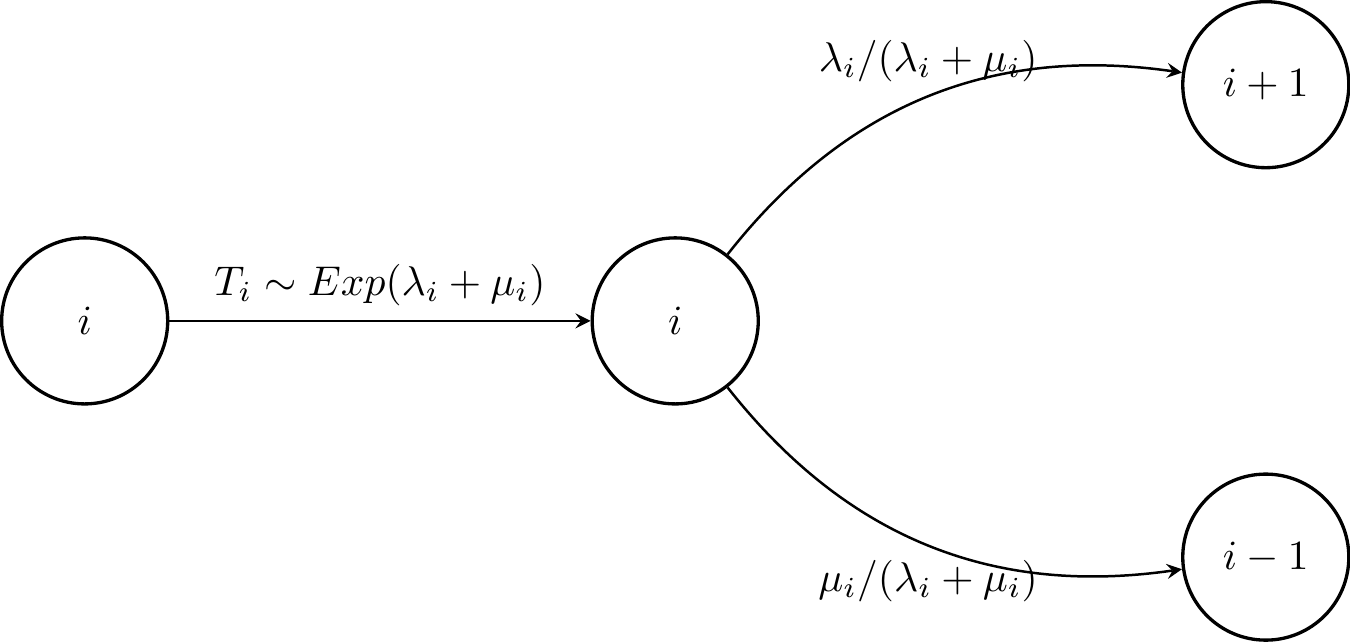
\includegraphics[width=0.5\linewidth]{index_files/figure-latex/fig7-1} \end{center}

Uma possível realização de \(X_t\) é:
\[i \longrightarrow i+1 \longrightarrow i \longrightarrow i-1 \longrightarrow \dots\]

O movimento é análogo ao do caminho aleatório, com a diferença de que o tempo de espera em cada estado é uma v.a. com distribuição exponencial.
\end{remark}

\subsection{Equações diferenciais de processos de nascimento e morte}\label{equacoes-diferenciais-de-processos-de-nascimento-e-morte}

As equações de Chapman-Kolmogorov descrevem a evolução das probabilidades de transição ao longo do tempo. A partir destas equações, podemos deduzir as equações diferenciais que descrevem a evolução das probabilidades de transição em função do tempo.

\(\,\)

Pela relação \eqref{eq:chapkol}, temos:

\begin{align*}
P_{ij}(t+h) &= \sum_{k=0}^{+\infty} P_{ik}(h) \cdot P_{kj}(t) \\
            &= P_{ii}(h) \cdot P_{ij}(t) + P_{i,i+1}(h) \cdot P_{i+1,j}(t) + P_{i,i-1}(h) \cdot P_{i-1,j}(t) + \sum_{k \notin \{i-1,i,i+1\}} P_{ik}(h) \cdot P_{kj}(t) \\
            &= \left(1 - (\lambda_i + \mu_i) h\right) P_{ij}(t) + \lambda_i h \cdot P_{i+1,j}(t) + \mu_i h \cdot P_{i-1,j}(t) + o(h),
\end{align*}

assumindo que o processo é de saltos de primeiro vizinho, isto é, que \(P_{ik}(h) = o(h)\) para \(|k - i| \geq 2\).

Dividindo por \(h\) e aplicando o limite quando \(h \to 0\), obtemos:

\begin{equation*}
\boxed{
P'_{ij}(t) = \lambda_i P_{i+1,j}(t) + \mu_i P_{i-1,j}(t) - (\lambda_i + \mu_i) P_{ij}(t), \quad i \geq 1.
}
\end{equation*}

Para \(i = 0\), temos:

\begin{align*}
P_{0j}(t+h) &= P_{00}(h) \cdot P_{0j}(t) + P_{0,1}(h) \cdot P_{1j}(t) + \sum_{k \geq 2} P_{0k}(h) \cdot P_{kj}(t) \\
            &= \left(1 - \lambda_0 h\right) P_{0j}(t) + \lambda_0 h \cdot P_{1j}(t) + o(h),
\end{align*}

donde se obtém:

\begin{equation*}
\boxed{
P'_{0j}(t) = \lambda_0 P_{1j}(t) - \lambda_0 P_{0j}(t).
}
\end{equation*}

Estas equações designam-se por \textbf{Equações de Kolmogorov de atraso}, e descrevem como a probabilidade de transição evolui em função do \textbf{estado inicial} \(i\).

As condições iniciais associadas são:
\[
P_{ij}(0) = \delta_{ij}, \quad i,j \in \mathbb{N}_0,
\]
onde \(\delta_{ij}\) representa o delta de Kronecker.

\(\,\)

Por outro lado, a equação de Chapman-Kolmogorov \eqref{eq:chapkol} também pode ser escrita na forma:

\begin{align*}
P_{ij}(t+h) &= \sum_{k=0}^{+\infty} P_{ik}(t) \cdot P_{kj}(h) \\
            &= P_{ij}(t) \cdot P_{jj}(h) + P_{i,j+1}(t) \cdot P_{j+1,j}(h) + P_{i,j-1}(t) \cdot P_{j-1,j}(h) + \sum_{k \notin \{j-1,j,j+1\}} P_{ik}(t) \cdot P_{kj}(h) \\
            &= \left(1 - (\lambda_j + \mu_j) h \right) P_{ij}(t) + \lambda_{j-1} h \cdot P_{i,j-1}(t) + \mu_{j+1} h \cdot P_{i,j+1}(t) + o(h),
\end{align*}

assumindo, tal como anteriormente, que os saltos ocorrem apenas entre estados vizinhos.

Dividindo por \(h\) e aplicando o limite \(h \to 0\), obtemos:

\begin{equation*}
\boxed{
P'_{ij}(t) = \lambda_{j-1} P_{i,j-1}(t) + \mu_{j+1} P_{i,j+1}(t) - (\lambda_j + \mu_j) P_{ij}(t), \quad j \geq 1.
}
\end{equation*}

Para \(j = 0\), temos:

\begin{equation*}
\boxed{
P'_{i0}(t) = \mu_1 P_{i1}(t) - \lambda_0 P_{i0}(t).
}
\end{equation*}

Estas equações designam-se por \textbf{Equações de Kolmogorov de avanço}, e descrevem como a probabilidade de transição evolui em função do \textbf{estado final} \(j\).

\(\,\)

Vejamos agora se o comportamento de \(P_{ij}(t)\) estabiliza à medida que \(t \to +\infty\).

É possível demonstrar (ver, por exemplo, Karlin \& Taylor) que, sob condições adequadas (recorrência positiva e aperiocidade), as probabilidades de transição convergem para um valor limite, isto é:

\[
\lim_{t \to +\infty} P_{ij}(t) = \pi_j,
\]
onde \(\pi_j\) é a probabilidade de que o sistema se encontre no estado \(j\) em regime estacionário, independentemente do estado inicial \(i\).

Por outras palavras, \(\pi_j\) representa a probabilidade limite de que o sistema se encontre no estado \(j\), num instante arbitrário no futuro.

\(\,\)

Neste caso, as equações de Kolmogorov de atraso (ou avanço) convergem para um sistema de equações algébricas conhecidas como \textbf{Equações de Kolmogorov estacionárias}, que descrevem o comportamento assintótico do processo de nascimento e morte:

\[
\boxed{
\begin{cases}
\lambda_0 \pi_1 - \lambda_0 \pi_0 = 0, & j = 0, \\
\lambda_{j-1} \pi_{j-1} + \mu_{j+1} \pi_{j+1} - (\lambda_j + \mu_j) \pi_j = 0, & j \geq 1.
\end{cases}}
\]

Estas equações, a par da condição de normalização
\[
\sum_{j=0}^{\infty} \pi_j = 1,
\]
permitem determinar a distribuição de probabilidade estacionária \((\pi_j)_{j \in \mathbb{N}_0}\).

\(\,\)

\begin{exercise}
\leavevmode

Considere um sistema de self-service em que a probabilidade de haver uma chegada em \((t,t+h)\) dado que existem \(j\) Clientes a servirem-se no instante \(t\) é igual a \(ajh+o(h), ~j \geq 0,\) quando \(h \to 0\), onde \(a>0\) é uma constante real positiva. Suponha que os Clientes acabam o seu serviço segundo um processo de Poisson de intensidade \(2a\) e que estão reunidas todas as condições para poder modelar o sistema por um processo de nascimento e morte, \(N_t\).

\begin{enumerate}
\def\labelenumi{\alph{enumi})}
\item
  Identifique um conjunto de axiomas que caracterize o processo \((M_t: ~t \geq 0)\), onde \(M_t\) representa o número de Clientes que acabam de se servirem num intervalo de tempo de amplitude \(t\).
\item
  Identifique, justificando, as taxas de nascimento e morte do processo \(N_t\).
\item
  Faça um diagrama de velocidade de probabilidades de transição para o processo \(N_t\) e escreva o correspondente sistema de equações de avanço de Kolmogorov.
\end{enumerate}

\end{exercise}

\begin{exercise}
\leavevmode

Considere que os autocarros chegam a uma certa rua segundo um processo de Poisson de intensidade de 10 por hora, e que percorrem num intervalo de tempo que é sempre constante e igual a 10 minutos. Suponha que a rua não tem limitação para o número de veículos que nela podem transitar.

\begin{enumerate}
\def\labelenumi{\alph{enumi})}
\item
  Após associar ao problema um processo de nascimento e morte, determine a distribuição de equilíbrio e interprete o significado de \(\pi_0\).
\item
  Determine o número médio de autocarros na rua depois de terem decorrido algumas horas desde o início da carreira.
\item
  O número de autocarros tende a aumentar ou a diminuir com a passagem do tempo? Justifique.
\end{enumerate}

\end{exercise}

\(\,\)

\begin{exercise}
\leavevmode

Seja \((X(t), ~t\geq 0)\) um processo de nascimento e morte tal que:
\[
\begin{array}{rclcc}
\lambda _{n} & = & \lambda q^{n} & 0<q<1,\;\lambda >0 & n=0,1,2,\cdots \\
\mu _{n} & = & \mu & \mu >0 & n=1,2,\cdots \\
\mu _{0} & = & 0 &  & \
\end{array}
\]
Designe por \(P_{n}(t)=P(X(t)=n)\). Prove que

\begin{eqnarray*}
P_{0}^{\prime }(t) &=&-\lambda P_{0}(t)+\mu P_{1}(t) \\
P_{n}^{\prime }(t) &=&\lambda q^{n-1}P_{n-1}(t)-(\lambda q^{n}+\mu
)P_{n}(t)+\mu P_{n+1}(t),\;\;\;n\geq 1.
\end{eqnarray*}

\end{exercise}

\(\,\)

\begin{exercise}
\leavevmode

Considere o processo estocástico \(N(t)\), que representa o número de linhas ocupadas numa central telefónica, a qual dispõe de um número elevado de linhas. Este processo é modelado por um sistema com chegadas espontâneas de chamadas e término aleatório de chamadas, com os seguintes pressupostos:

\begin{itemize}
\item
  As chamadas chegam à central a uma taxa constante \(\lambda\), independentemente do número de linhas atualmente ocupadas.
\item
  Cada chamada em curso termina a uma taxa \(\mu\), de forma independente das restantes. Assim, quando há \(k\) chamadas em curso (ou \(k\) linhas ocupadas), a taxa total de término é \(k\,\mu\).
\end{itemize}

\begin{enumerate}
\def\labelenumi{(\alph{enumi})}
\item
  Mostre que as Equações de Kolmogorov de avanço associadas às probabilidades \(P_i(t) = P(N(t) = i)\) são dadas por:
  \[
  P_i'(t) = -(\lambda + i\,\mu)\,P_i(t) + \lambda\,P_{i-1}(t) + (i+1)\mu\,P_{i+1}(t), \quad i = 0,1,2,\ldots
  \]
\item
  Suponha que, para cada \(i \in \mathbb{N}_0\), a função \(P_i(t)\) é dada por:
  \[
  P_i(t) = \frac{(\lambda/\mu)^i}{i!} \left( 1 - e^{-\mu t} \right)^i \exp\left\{ -\frac{\lambda}{\mu} \left( 1 - e^{-\mu t} \right) \right\}, \quad i = 0,1,2,\ldots
  \]
  Determine a probabilidade de todas as linhas estarem desocupadas no regime estacionário (isto é, quando \(t \to +\infty\)), e deduza a forma da distribuição estacionária do número de linhas ocupadas.
\end{enumerate}

\end{exercise}

\(\,\)

\begin{exercise}
\leavevmode

Seja \(Y_n\), \(n = 0,1,\ldots\), uma cadeia de Markov com espaço de estados \(E = \{0,1\}\) e matriz de transição \(\mathbb{P}\) dada por:
\[
\mathbb{P} =
\begin{bmatrix}
0 & 1 \\
1 - \alpha & \alpha
\end{bmatrix}.
\]

Considere ainda um processo de Poisson com parâmetro \(\lambda\), isto é, \((N(t),\, t \geq 0)\). Mostre que o processo definido por \(X(t) = Y_{N(t)}\), para \(t \geq 0\), é um processo de nascimento e morte com dois estados, e determine os parâmetros \(\lambda_0\) e \(\mu_1\) em função de \(\alpha\) e \(\lambda\).

\end{exercise}

\chapter{Complementos de processos estocásticos}\label{complementos-de-processos-estocasticos}

\section{Processo de Wiener}\label{processo-de-wiener}

\begin{definition}[Filtração]
Seja \(X = (X(t), ~ t \in T)\) um processo estocástico definido no espaço de probabilidade \((\Omega, \mathcal{F}, P)\), com conjunto de índices \(T = [0, +\infty[\). Uma família de sub-\(\sigma\)-álgebras de \(\mathcal{F}\), tal que para \(s \leq t\) se tenha \(\mathcal{F}_s \subset \mathcal{F}_t\), designa-se por \textbf{filtração}.

Denomina-se \textbf{filtração natural} do processo \(X\) a família\\
\[
\left(\mathcal{F}_t = \sigma\big(X_s : 0 \leq s \leq t\big), \; t \in T\right),
\]\\
formada pelas álgebras-\(\sigma\) geradas pelo processo \(X\) até ao instante \(t\).

Um processo estocástico \(X = (X(t), ~ t \in T)\) está \textbf{adaptado} à filtração \((\mathcal{F}_t, t \in T)\) se, para todo \(t \in T\), a variável aleatória \(X(t)\) é \(\mathcal{F}_t\)-mensurável, isto é, as imagens inversas dos conjuntos \(B \in \mathcal{B}\) estão contidas em \(\mathcal{F}_t\).
\end{definition}

\(\,\)

Em 1828, o botânico inglês Robert Brown observou pequenas partículas de pólen imersas num líquido a movimentarem-se de forma completamente aleatória. Mais tarde, em 1905, Albert Einstein justificou este movimento com a constante colisão entre as partículas e as moléculas do líquido envolvente e caracterizou-o por um processo estocástico que viria a ser chamado processo de Wiener. Finalmente, em 1918, apareceu a primeira definição matemática do termo através do matemático Norbert Wiener.m

\(\,\)

\begin{definition}[Processo de Wiener padrão (ou movimento Browniano)]

Um \textbf{processo de Wiener padrão} (ou \textbf{movimento Browniano}) é um processo estocástico \(W = (W_t)_{t \geq 0}\) definido num espaço de probabilidade \((\Omega, \mathcal{F}, P)\), que satisfaz as seguintes propriedades:

\begin{enumerate}
\def\labelenumi{\arabic{enumi}.}
\item
  \textbf{Condição inicial:} \(W_0 = 0\) quase certamente, isto é,\\
  \[
  P(W_0 = 0) = 1;
  \]
\item
  \textbf{Incrementos gaussianos:} Para quaisquer instantes \(0 \leq s < t < \infty\), a variável aleatória \(W_t - W_s\) é normalmente distribuída com média zero e variância \(t - s\), ou seja,\\
  \[
  W_t - W_s \sim \mathcal{N}(0, t - s);
  \]
\item
  \textbf{Incrementos independentes:} Para todo \(n \in \mathbb{N}\) e qualquer sequência crescente de instantes \(0 \leq t_0 < t_1 < \dots < t_n\), os incrementos\\
  \[
  W_{t_1} - W_{t_0}, \; W_{t_2} - W_{t_1}, \; \dots, \; W_{t_n} - W_{t_{n-1}}
  \]\\
  são variáveis aleatórias independentes;
\item
  \textbf{Trajetórias contínuas:} Com probabilidade 1, a aplicação \(t \mapsto W_t(\omega)\) é contínua para todo \(\omega \in \Omega\), ou seja,\\
  \[
  P\left( W \in C([0, \infty[) \right) = 1,
  \]\\
  onde \(C([0, \infty[)\) denota o espaço das funções contínuas em \([0, \infty[\).
\end{enumerate}

\end{definition}

\(\,\)

Nos processos estocásticos e, em particular, nas equações diferenciais estocásticas, o processo de Wiener representa o efeito acumulado das perturbações aleatórias na evolução de determinado fenómeno em estudo. Dada a importância deste processo, iremos apresentar algumas das suas propriedades.

\(\,\)

\begin{definition}

Considere-se uma função \(f:[0,t] \rightarrow \mathbb{R}\) e uma sequência de partições \(\mathcal{P}_n = \{t_0^n, t_1^n, \ldots, t_n^n\}\) do intervalo \([0,t]\), com \(0 = t_0^n < t_1^n < \cdots < t_n^n = t\) para cada \(n \in \mathbb{N}\), tais que
\[
\delta_n = \max_{0 \leq i \leq n-1} |t_{i+1}^n - t_i^n| \to 0 \quad \text{quando } n \to +\infty.
\]

\begin{itemize}
\item
  A \textbf{variação} da função \(f\) no intervalo \([0,t]\) é definida por
  \[
  V_f([0,t]) = V_f(t) := \lim_{n \to +\infty} \sum_{i=0}^{n-1} |f(t_{i+1}^n) - f(t_i^n)|.
  \]
\item
  Diz-se que \(f\) tem \textbf{variação finita} no intervalo \([0,t]\) se \(V_f(t) < +\infty\).
\item
  Diz-se que \(f\) tem \textbf{variação limitada} no intervalo \([0,t]\) se
  \[
  \sup_{u \in [0,t]} V_f(u) < k, \quad \text{para algum } k > 0.
  \]
\item
  Diz-se que \(f\) tem \textbf{variação quadrática} no intervalo \([0,t]\) se existir e for finito o limite
  \[
  V_f^2(t) := \lim_{n \to +\infty} \sum_{i=0}^{n-1} |f(t_{i+1}^n) - f(t_i^n)|^2.
  \]
\end{itemize}

\end{definition}

\(\,\)

\begin{proposition}[Propriedades do processo de Wiener]

O processo de Wiener, \(W_t\), possui as seguintes propriedades:

\begin{enumerate}
\def\labelenumi{\arabic{enumi}.}
\item
  Existe uma versão separável e contínua do processo, isto é, com trajectórias quase certamente contínuas;
\item
  Para todo \(t \geq 0\), \(W_t \sim \mathcal{N}(0,t);\)
\item
  A função de covariância é dada por \(Cov[W_s, W_t] = E[W_s W_t] = s \wedge t;\)
\item
  \(W_t\) é um processo de Markov homogéneo;
\item
  A distribuição condicional de \(W_{s+\tau}\) dado \(W_s = x\) é Normal com média \(x\) e variância \(\tau\);
\item
  \(W_t\) é uma martingala em relação à sua filtração natural;
\item
  As trajectórias do processo de Wiener são, quase certamente, não diferenciáveis;
\item
  As trajectórias do processo de Wiener são, quase certamente, de variação ilimitada em qualquer intervalo;
\item
  Possui variação quadrática finita no intervalo \([a,b]\), igual a \(b-a\).
\end{enumerate}

\end{proposition}

\(\,\)

\begin{remark}[Ruído branco como derivada generalizada do processo de Wiener]
Embora as trajectórias do processo de Wiener sejam, quase certamente, contínuas mas não diferenciáveis (propriedade 7), e tenham variação total infinita (propriedade 8), é possível interpretar a sua derivada no \textbf{sentido das distribuições generalizadas} (ou distribuições de Schwartz).

Neste contexto, define-se a \textbf{derivada generalizada} do processo de Wiener como
\[
\frac{dW_t}{dt} = \xi_t,
\]
onde \(\xi_t\) representa um \textbf{processo estocástico generalizado}, designado por \textbf{ruído branco} (ou \emph{white noise}). Este processo não é uma função no sentido clássico, mas sim uma distribuição (ou funcional) que actua sobre funções teste suaves.

O ruído branco \(\xi_t\) caracteriza-se pelas seguintes propriedades formais:

\begin{itemize}
\tightlist
\item
  É um processo com média nula: \(E(\xi_t) = 0\);
\item
  A sua função de autocovariância é dada por:
  \[
  E(\xi_s \xi_t) = \delta(t - s),
  \]
  onde \(\delta\) é a função delta de Dirac, interpretada como distribuição.
\end{itemize}

Este formalismo é essencial na formulação de equações diferenciais estocásticas (EDEs), nas quais o ruído branco representa uma força aleatória infinitesimalmente perturbadora que actua continuamente ao longo do tempo.
\end{remark}

\(\,\)

Na imagem seguinte apresentam-se duas trajectórias de um processo de Wiener. As trajectórias foram obtidas por simulação numérica, considerando incrementos independentes e normalmente distribuídos com média zero e variância proporcional ao incremento temporal.

\pandocbounded{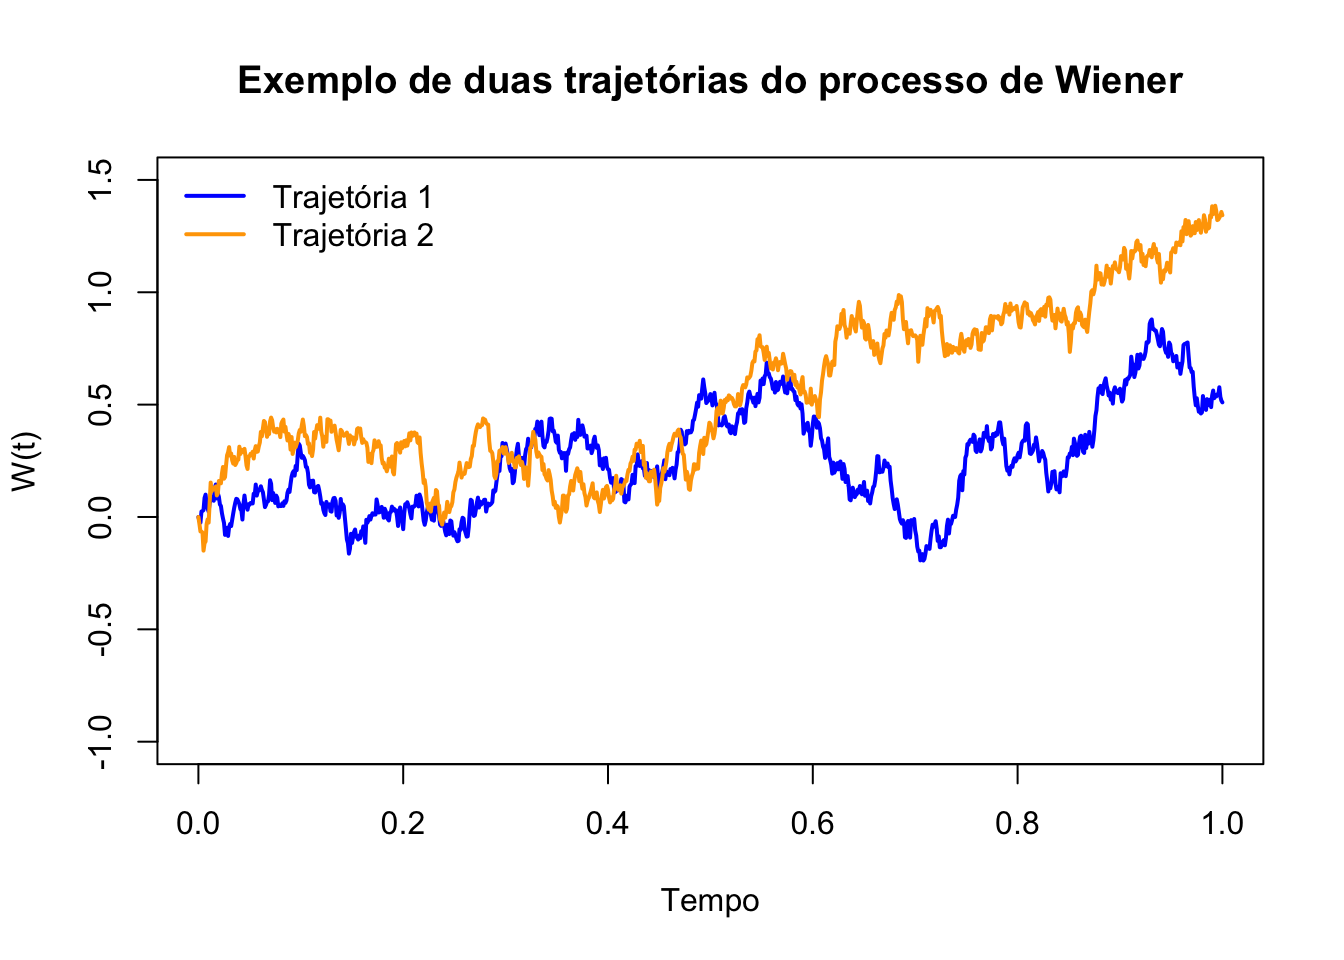
\includegraphics[keepaspectratio]{index_files/figure-latex/fig-wiener-trajectories-1.pdf}}

\(\,\)

\begin{exercise}[Braumann (2005)]

Tirando partido das propriedades do processo de Wiener, calcule ou determine:

\begin{enumerate}
\def\labelenumi{\arabic{enumi}.}
\item
  \(P(W(2.7) > 1.5)\).
\item
  \(P(-1.5 < W(2.7) < 1.5)\).
\item
  \(P(W(2.7) < 1.5 \mid W(1.8) = 1)\).
\item
  \(P(-1.5 < W(2.7) < 1.5 \mid W(1.8) = 1)\).
\item
  \(E(W(t) \mid W(s), W(u)) \quad \text{com } 0 < u < s < t\).
\item
  \(Var(W(t) \mid W(s), W(u)) \quad \text{com } 0 < u < s < t\).
\item
  \(P(W(2.7) > 1.5 \mid W(1.8) = 1,\, W(0.5) = -2)\).
\item
  \(E(W(2.7) \mid W(1.8) = 1,\, W(0.5) = -2)\).
\item
  \(P(W(1.8) < 1 \mid W(2.7) = 1.5)\).
\item
  \(P(W(1.8) = 1 \mid W(2.7) < 1.5)\).
\item
  \(P(W(2.7) = 1.5,\, W(1.8) > 1)\).
\item
  \(P(W(2.7) < 1.5,\, W(1.8) = 1)\).
\item
  \(P(-1 < W(2.7) - W(1.8) < 1.4 \;\wedge\; 0.5 < W(1.6) - W(0.9) < 1.5)\).
\item
  \(P(-1 < W(2.7) - W(1.8) < 1.4 \mid W(1.6) - W(0.9) = 1.5)\).
\end{enumerate}

\end{exercise}

\(\,\)

\begin{exercise}
\leavevmode

Considere um movimento Browniano standard \((B(t), ~t\geq 0)\) nos instantes \(0<u<u+v<u+v+w\), em que \(u,v,w>0\). Calcule
\[
E(B(u)B(u+v)B(u+v+w)).
\]

\end{exercise}

\(\,\)

\begin{exercise}
\leavevmode

Seja \((B(t), ~t\geq 0)\) com \(B(0)\equiv 3\), um movimento Browniano com variância \(\sigma^{2}\). Determine
\[
Cov(B(t),B(s)), \quad t,s \geq 0.
\]

\end{exercise}

\(\,\)

\begin{exercise}
\leavevmode

Considere um movimento Browniano standard \((B(t), ~t\geq 0)\). Determine as funções de covariância para os processos estocásticos seguintes:

\begin{enumerate}
\def\labelenumi{(\alph{enumi})}
\item
  \(U(t)=e^{-t}B(e^{2t})\), \(~t\geq 0\).
\item
  \(V(t)=(1-t)B\left(\dfrac{t}{1-t}\right)\), para \(0<t<1\).
\item
  \(W(t)=tB\left(\dfrac{1}{t}\right)\), com \(W(0)=0\).
\end{enumerate}

\end{exercise}

\(\,\)

\begin{exercise}
\leavevmode

Considere um movimento Browniano standard \((B(t), ~t \geq 0)\). Para \(t\) fixo e \(M(t)=\max\limits_{0\leq u\leq t}B(u)\), mostre que:

\begin{enumerate}
\def\labelenumi{(\alph{enumi})}
\item
  \(M(t)\) e \(\left| B(t)\right|\) têm a mesma distribuuição com f.d.p.
  \[
  f_{M(t)}(x)=\frac{2}{\sqrt{t}}\phi (x/\sqrt{t}),  ~ x>0.
  \]
\item
  \(E(M(t))=\sqrt{2t/\pi }\).
\end{enumerate}

\end{exercise}

\(\,\)

\begin{exercise}
\leavevmode

Sejam \(B_{1}(t)\) e \(B_{2}(t)\) dois movimentos Brownianos independentes e \(R(t)=\sqrt{B_{1}(u)^{2}+B_{2}(u)^{2}},\) \(t\geq 0\). Calcule \(E(R(t)).\)

\end{exercise}

\(\,\)

\begin{exercise}
\leavevmode

As flutuações de preço das acções de determinada companhia são modeladas por um movimento Browniano \((A(t),\, t \geq 0)\). Suponha que a companhia entra em falência se o preço de mercado das acções atingir o nível zero.

Se o valor inicial das acções for \(A(0) = 5\) u.m., determine a probabilidade de \ldots{}

\begin{enumerate}
\def\labelenumi{(\alph{enumi})}
\item
  \ldots{} a companhia entrar em falência no instante \(t = 25\).
\item
  \ldots{} as acções estarem acima de 10 unidades monetárias no instante \(t = 25\).
\end{enumerate}

\end{exercise}

\(\,\)

\begin{exercise}
\leavevmode

Considere um movimento Browniano com parâmetros \(\mu=0.1\) e \(\sigma =2\). Calcule a probabilidade do processo sair fora do intervalo \((a,b]\) no ponto \(b\), partindo de \(X(0)=0\), para \(b=1,10,100\) e \(a=-b\).

\end{exercise}

\(\,\)

\begin{exercise}
\leavevmode

A flutuação do preço de determinado tipo de acções pode ser descrita por um movimento browniano geométrico com desvio-padrão \(\alpha = 0\). Supondo que adquire estas acções, quais são as hipóteses de ver o seu capital investido duplicar?

\end{exercise}

\section{O integral de Itô}\label{o-integral-de-ito}

\begin{remark}
No que se segue, adoptámos a seguinte notação para esperança matemática e probabilidade condicionadas:

\[E(\cdot \mid X_s=x)=E_{s,x}(\cdot)\]
e
\[P(\cdot \mid X_s=x)=P_{s,x}(\cdot).\]
\end{remark}

\(\,\)

\begin{definition}[Processo de difusão]
Seja \((\Omega,\mathcal{F},P)\) um espaço de probabilidade e \((X_t, t \geq 0)\) um processo estocástico definido nesse espaço. Diz-se que \(X_t\) é um \textbf{processo de difusão} se satisfizer as seguintes propriedades:

\begin{enumerate}
\def\labelenumi{\roman{enumi})}
\item
  \(X_t\) é um processo de Markov;
\item
  As trajectórias de \(X_t\) são quase certamente contínuas;
\item
  \(X_t \in L^2\), isto é, \(E[X_t^2] < +\infty\);
\item
  Para todo \(\varepsilon > 0\), tem-se
  \[
  \lim_{\Delta \to 0^+} \frac{P_{s,x}(|X_{s+\Delta} - X_s| > \varepsilon)}{\Delta} = 0;
  \]
\item
  Existe, e é finito, o limite
  \[
  \lim_{\Delta \to 0^+} E_{s,x}\left[\frac{X_{s+\Delta} - X_s}{\Delta}\right] = a(s,x);
  \]
\item
  Existe, e é finito, o limite
  \[
  \lim_{\Delta \to 0^+} E_{s,x}\left[\frac{(X_{s+\Delta} - X_s)^2}{\Delta}\right] = b(s,x).
  \]
\end{enumerate}

Se as funções \(a(s,x)\) e \(b(s,x)\) forem independentes da variável temporal \(s\), o processo diz-se \textbf{homogéneo}.

As funções \(a(s,x)\) e \(b(s,x)\) designam-se, respectivamente, por \textbf{coeficiente de tendência} (ou \textbf{momento infinitesimal de primeira ordem}) e \textbf{coeficiente de difusão} (ou \textbf{momento infinitesimal de segunda ordem}).

O coeficiente de tendência, \(a(s,x)\), mede a velocidade da média do processo no instante \(s\), enquanto que o coeficiente de difusão, \(b(s,x)\), mede a intensidade das flutuações do processo, ou seja, mede a velocidade da variância do processo no instante \(s\).

\emph{Nota:} Existem na literatura definições alternativas para processo de difusão, algumas das quais assumem hipóteses adicionais ou diferentes.
\end{definition}

\(\,\)

\begin{exercise}[Fonte: Braumann (2005)]
\leavevmode

\begin{enumerate}
\def\labelenumi{(\roman{enumi})}
\item
  Mostre que o processo de Wiener \(W_t\) é um processo de difusão homogéneo com coeficiente de tendência nulo e coeficiente de difusão unitário.
\item
  Mostre que \(X_t = x_0 + \sigma W_t\), com \(x_0\) e \(\sigma\) constantes, sendo um processo de Wiener (não-padrão), é um processo de difusão homogéneo com coeficiente de tendência nulo e coeficiente de difusão \(\sigma^2\).
\item
  Mostre que \(Z_t = x_0 + \mu t + \sigma W_t\), com \(x_0\), \(\mu\) e \(\sigma\) constantes, conhecido como movimento browniano com tendência, é um processo de difusão homogéneo com coeficiente de tendência \(\mu\) e coeficiente de difusão \(\sigma^2\).
\end{enumerate}

\end{exercise}

\(\,\)

\begin{definition}[Função delta de Dirac]

Chama-se \textbf{função delta de Dirac} à função generalizada \(\delta(x)\) com as seguintes propriedades:

\begin{enumerate}
\def\labelenumi{\arabic{enumi}.}
\item
  \(\delta(x) = 0\), para todo o \(x \neq 0\);
\item
  \(\delta(0) = +\infty\);
\item
  \(\displaystyle \int_{-\infty}^{+\infty} \delta(x)\,dx = 1\).
\end{enumerate}

\end{definition}

\(\,\)

A caraterização, do ponto de vista probabilístico, de um processo de difusão recorre apenas aos seus momentos infinitesimais e às equações de Kolmogorov.

\(\,\)

\begin{theorem}

Seja \(X_t\) um processo de difusão, como definido anteriormente, com função densidade de transição \(p(t, y \mid s, x)\), contínua em \(s\), com derivadas parciais de primeira e segunda ordem em relação a \(x\) finitas e contínuas em \(s\). Nessas condições, verificam-se:

\begin{enumerate}
\def\labelenumi{\arabic{enumi}.}
\item
  \textbf{Equação de Kolmogorov progressiva} (ou \textbf{equação de Fokker-Planck}):
  \[
  \frac{\partial p}{\partial t} + \frac{\partial\big(a(s,x)\,p\big)}{\partial y} - \frac{1}{2} \frac{\partial^2\big(b(s,x)\,p\big)}{\partial y^2} = 0,
  \]
  com condição inicial
  \[
  \lim_{t \downarrow s} p(t, y \mid s, x) = \delta(x - y),
  \]
  onde \(\delta\) representa a função delta de Dirac, e \((s, x)\) está fixo;
\item
  \textbf{Equação de Kolmogorov regressiva}:
  \[
  \frac{\partial p}{\partial s} + a(s,x)\,\frac{\partial p}{\partial x} + \frac{1}{2}\,b(s,x)\,\frac{\partial^2 p}{\partial x^2} = 0,
  \]
  com condição inicial
  \[
  \lim_{t \uparrow s} p(t, y \mid s, x) = \delta(x - y),
  \]
  onde \(\delta\) representa a função delta de Dirac, e \((t, y)\) está fixo.
\end{enumerate}

\end{theorem}

\(\,\)

Considere-se o ponto \(X(0) = X_0 \in \mathbb{R}\) e o seguinte problema de Cauchy, induzido por uma equação diferencial ordinária:

\[
\begin{cases}
dX(t) = f(X(t))\,dt, & \text{para } t > 0, \\
X(0) = X_0, &
\end{cases}
\label{eq:odeex}
\]

onde \(f: \mathbb{R} \rightarrow \mathbb{R}\) é uma função diferenciável, e \(X: \mathbb{R}_0^+ \rightarrow \mathbb{R}\) é a solução do problema \eqref{eq:odeex}.

Se interpretarmos \(X(t)\) como a trajectória de uma partícula, então \(dX(t)/dt\) representa a sua velocidade. É natural admitir que essa velocidade apresente pequenas oscilações que não são explicadas pela função \(f\), ou seja, o sistema descrito na equação \eqref{eq:odeex} não incorpora o efeito aleatório que as flutuações ambientais induzem na trajectória de \(X\). Assim, torna-se necessário adicionar um \emph{ruído} ao problema \eqref{eq:odeex}, de modo a reflectir a influência dessas flutuações sobre a dinâmica do sistema:

\[
\begin{cases}
dX(t) = f(X(t))\,dt + g(X(t))\,\xi(t)\,dt, & \text{para } t > 0, \\
X(0) = X_0, &
\end{cases}
\label{eq:sdeex}
\]

onde \(g(\cdot)\), que mede a intensidade das flutuações ambientais, é uma função dependente de \(X(t)\).

Considerando que \(dW(t) = \xi(t)\,dt\), o sistema \eqref{eq:sdeex} pode reescrever-se da seguinte forma:

\[
\begin{cases}
dX(t) = f(X(t))\,dt + g(X(t))\,dW(t), \\
X(0) = X_0,
\end{cases}
\]

o qual representa uma \textbf{Equação Diferencial Estocástica (EDE)}. A solução deste sistema é dada por:

\[
X(t) = X_0 + \int_{0}^{t} f(X(s))\,ds + \int_{0}^{t} g(X(s))\,dW(s), \quad t > 0,
\label{eq:sdesol}
\]

em que o primeiro integral é um integral de Riemann-Stieltjes. Contudo, o segundo integral \textbf{não existe} neste sentido, dado que as trajectórias do processo de Wiener são, quase certamente, de variação ilimitada no intervalo \([0,t]\).

No entanto, como o processo de Wiener possui variação quadrática finita, é possível definir o segundo integral recorrendo à \textbf{definição de integral estocástico}.

Note-se que, como já referido, se omitiu a dependência explícita em \(\omega\) na notação de \(X(t)\).

Mostraremos de seguida como obter a solução \eqref{eq:sdesol}, bem como a definição do integral estocástico
\[
\int_{0}^{t} g(X(s))\,dW(s).
\]

\(\,\)

Suponhamos que desejamos calcular o seguinte integral:

\[
\int_{0}^{t} W(t)\,dW(t).
\]

Se aplicarmos as regras de cálculo habituais, obtemos como solução:

\[
\frac{1}{2}W^2(t).
\label{eq:solintw}
\]

Vamos verificar se esta solução está correta.

Seja \(f:[0,t] \rightarrow \mathbb{R}^{+}\), com \(f(u) = W(u)\), uma função, e sejam \(\mathcal{P}_n = \{t_0^n, t_1^n, \ldots, t_n^n\}\), \(n = 1,2,\ldots\), partições do intervalo \([0,t]\) com\\
\[
0 = t_0^n < t_1^n < \ldots < t_n^n = t \geq 0,
\]
tais que os diâmetros\\
\[
\delta_n = \max_{0 \leq i \leq n-1} |t_{i+1}^n - t_i^n|
\]\\
satisfazem \(\delta_n \to 0\) quando \(n \to +\infty\).

Consideremos as somas de Riemann-Stieltjes aproximadoras do integral \(\int_{0}^{t} f(u)\,dW(u)\):
\[
\sum_{i=0}^{n-1} W(\xi_i^n)\big(W(t_{i+1}^n) - W(t_i^n)\big),
\]
com \(\xi_i^n \in [t_i^n, t_{i+1}^n]\), e usemos limites em média quadrática quando \(n \to +\infty\) como possível definição do integral.

Consideremos o caso particular \(\xi_i^n = (1 - \lambda)t_i^n + \lambda t_{i+1}^n\), e definamos as somas de Riemann-Stieltjes:

\[
S_{\lambda}(W(t)) = \sum_{i=0}^{n-1} W(\xi_i^n)\big(W(t_{i+1}^n) - W(t_i^n)\big).
\]

Facilmente verificamos que, para \(\lambda\) fixo, o limite em média quadrática destas somas, quando \(n \to +\infty\), é

\[
\frac{W^2(t)}{2} + \left(\lambda - \frac{1}{2}\right)t.
\]

Com efeito:

\[
E\left[\left(S_{\lambda}(W(t)) - \frac{W^2(t)}{2} - \left(\lambda - \frac{1}{2}\right)t\right)^2\right] \longrightarrow 0.
\]

Este limite depende da escolha do valor de \(\lambda\) e, consequentemente, do ponto intermédio \(\xi_i \in [t_i, t_{i+1}]\). Assim, \textbf{não existe} o integral no sentido de Riemann-Stieltjes, pois falha a existência de um limite comum para todas as escolhas de pontos intermédios.

Ao fixarmos \(\lambda = 0\), obtemos como ponto intermédio o ponto inicial do intervalo, isto é, \(\xi_i = t_i\), e verificamos que

\[
\int_{0}^{t} W(t)\,dW(t) = \frac{1}{2}W^2(t) - \frac{1}{2}t,
\]

o que é um resultado \textbf{diferente} do indicado em \eqref{eq:solintw}. De facto, para diferentes valores de \(\lambda\), obtemos diferentes integrais. Por exemplo, se considerarmos \(\lambda = \frac{1}{2}\), o resultado do integral é:

\[
\int_{0}^{t} W(t)\,dW(t) = \frac{1}{2}W^2(t).
\]

O facto de diferentes valores de \(\lambda\) implicarem diferentes integrais levanta uma questão pertinente: \textbf{qual o valor de \(\lambda\) que devemos escolher?}

A escolha de \(\xi_i = t_i\), ou seja, o ponto inicial, permite-nos definir integrais de funções mais gerais do que apenas o processo de Wiener. Isto conduz a integrais do tipo:

\[
\int_{0}^{t} G(s)\,dW(s),
\]

onde \(G\) pertence a uma vasta classe de funções com a propriedade de serem \textbf{não-antecipativas}. Veremos mais à frente como definir rigorosamente estas funções.

Como se referiu, a escolha de \(\lambda\) permite obter diferentes integrais. Assim:

\begin{enumerate}
\def\labelenumi{(\roman{enumi})}
\item
  Se \(\lambda = 0\), escolhemos o ponto inicial do intervalo e obtemos o \textbf{integral de Itô};
\item
  Se \(\lambda = \frac{1}{2}\), escolhemos o ponto intermédio do intervalo e obtemos o \textbf{integral de Stratonovich}.
\end{enumerate}

\(\,\)

Vamos agora dedicar-nos ao estudo do integral de Itô. Começamos com a introdução de algumas definições e resultados importantes.

\(\,\)

\begin{definition}

Seja \(W(t),\ t \geq 0\), um processo de Wiener padrão definido num espaço de probabilidade \((\Omega, \mathcal{F}, P)\).

\begin{enumerate}
\def\labelenumi{\arabic{enumi}.}
\item
  Chama-se \textbf{filtração natural do processo de Wiener até ao instante} \(s > 0\) à \(\sigma\)-álgebra
  \[
  \mathcal{M}_s = \sigma(W(u),\ 0 \leq u \leq s);
  \]
\item
  Chama-se \textbf{\(\sigma\)-álgebra dos incrementos futuros do processo de Wiener} à \(\sigma\)-álgebra
  \[
  \mathcal{M}_s^+ = \sigma(W(u) - W(s),\ u \geq s);
  \]
\item
  Uma família \(\{ \mathcal{A}_s : 0 \leq s \leq t \}\) de \(\sigma\)-álgebras é chamada \textbf{filtração não-antecipativa}, relativamente a \(W(s)\), se:

  \begin{itemize}
  \item
    \(\mathcal{A}_s \supset \mathcal{M}_s,\quad 0 \leq s \leq t;\)
  \item
    \(\mathcal{A}_s\) é independente de \(\mathcal{M}_s^+,\ \forall s \geq 0.\)
  \end{itemize}
\end{enumerate}

\end{definition}

Informalmente, podemos dizer que a filtração \(\mathcal{A}_s\) contém toda a informação disponível do processo até ao instante \(s\).

A escolha da filtração não-antecipativa \(\mathcal{A}_s\) costuma coincidir com a própria filtração natural do processo de Wiener, \(\mathcal{M}_s\), desde que não seja necessário incluir informação adicional sobre o processo. Caso contrário, considera-se uma filtração \textbf{maior} (por exemplo, de modo a incluir a condição inicial de um problema de Cauchy), desde que a mesma seja não-antecipativa.

\(\,\)

\begin{definition}[Processo não-antecipativo]
Um processo estocástico \(G(t)\) é chamado de \textbf{não-antecipativo}, relativamente à filtração \(\mathcal{A}_t\), se \(G(t)\) é \(\mathcal{A}_t\)-mensurável, para todo \(t \geq 0\) (ou seja, \(G(t)\) depende apenas da informação disponível até ao instante \(t\)).
\end{definition}

\(\,\)

Tendo em conta estas definições, podemos definir o integral de Itô para uma classe especial de funções não-antecipativas, as \textbf{funções em escada}. Nota: na realidade, para definir o integral de Itô, não basta que \(G\) seja não-antecipativa. É necessário que \(G = G(t,\omega)\) seja \emph{conjuntamente mensurável}.

\(\,\)

\begin{definition}[Espaço de Hilbert]

Chama-se \textbf{espaço de Hilbert}, no intervalo \([0,t]\), e representa-se por \(H^2[0,t]\), ao espaço das funções
\[ G:[0,t] \times \Omega \rightarrow \mathbb{R} \]
que verificam as seguintes condições:

\begin{itemize}
\item
  \(G\) é \emph{conjuntamente mensurável} relativamente à medida de Lebesgue \(l\) em \([0,t]\) e à medida de probabilidade \(P\);
\item
  \(G\) é \textbf{não-antecipativa};
\item
  \(\displaystyle \int_{0}^{t}{E[G^2(u,\omega)]\,du} < +\infty\).
\end{itemize}

\end{definition}

\(\,\)

\begin{remark}
Nesta última definição considerámos, de modo abusivo, uma qualquer função \(G\) com a propriedade de ser conjuntamente mensurável relativamente às medidas \(l\) e \(P\).

Formalmente, deveríamos referir-nos ao conjunto das funções conjuntamente mensuráveis que sejam \textbf{quase iguais}, no seguinte sentido: duas funções \(G_1\) e \(G_2\) dizem-se quase iguais quando o conjunto de pontos \((t,\omega)\) onde diferem tem medida nula relativamente à medida produto \(l \times P\).

Assim, a função \(G\) é, na realidade, um \textbf{representante da classe de equivalência} das funções conjuntamente mensuráveis relativamente à relação de equivalência de quase-igualdade.

Deste modo, para simplificar a linguagem, referimo-nos à função \(G\) como um representante da classe de equivalência, em vez de referir explicitamente a própria classe de equivalência.
\end{remark}

\(\,\)

\begin{definition}[Função em escada]
Uma função \(G\), no espaço \(H^2[0,t]\), é chamada de \textbf{função em escada} se existir uma partição \(\{0 = t_0 < t_1 < \ldots < t_n = t\}\) do intervalo \([0,t]\) tal que:

\[
G(t) = G(t_i), \hspace{20pt} t_i \leq t \leq t_{i+1}, \hspace{5pt} i = 0, \ldots, n-1.
\]

Note-se que \(G(t_i)\) é \(\mathcal{A}_{t_i}\)-mensurável, pois \(G\) é não-antecipativa.

Ao espaço de funções em escada de \(H^2[0,t]\), chamamos \(H_E^2[0,t]\).
\end{definition}

\(\,\)

\begin{definition}[Integral de Itô para funções em escada]
Seja \(G\) uma função em \(H_E^2[0,t]\). O integral de Itô da função \(G\) no intervalo \([0,t]\) é dado por:

\[
\int_0^t G(s) \, dW(s) = \sum_{i=0}^{n-1} G(t_i)\left(W(t_{i+1}) - W(t_i)\right).
\]
\end{definition}

\(\,\)

\begin{theorem}[Propriedades do integral de Itô]

Sejam \(F\) e \(G\) duas funções em \(H_E^2[0,t]\), e \(\alpha, \beta \in \mathbb{R}\) duas constantes. Verificam-se as seguintes propriedades:

\begin{enumerate}
\def\labelenumi{\arabic{enumi}.}
\item
  Linearidade:
  \[
  \int_0^t \left(\alpha F(s) + \beta G(s)\right) \, dW(s)
  = \alpha \int_0^t F(s) \, dW(s) + \beta \int_0^t G(s) \, dW(s);
  \]
\item
  Esperança nula:
  \[
  E\left[\int_0^t F(s) \, dW(s)\right] = 0;
  \]
\item
  Isometria de Itô:
  \[
  E\left[\left(\int_0^t F(s) \, dW(s)\right)^2\right]
  = E\left[\int_0^t \left(F(s)\right)^2 \, ds\right]
  = \int_0^t E\left[\left(F(s)\right)^2\right] \, ds.
  \]
\end{enumerate}

\end{theorem}

\(\,\)

Definimos, assim, o integral de Itô para funções em escada, ou seja, funções no espaço \(H_E^2[0,t]\). Vamos agora generalizar este integral para funções genéricas em \(H^2[0,t]\), através da existência de sucessões aproximadoras de funções em escada.

\(\,\)

\begin{theorem}[Aproximação em média quadrática]
Seja \(G \in H^2[0,t]\) uma função. Então, existe uma sucessão de funções limitadas em escada, \(G_n \in H_E^2[0,t]\), tal que:

\[
E\left[\int_0^t |G(s) - G_n(s)|^2 \, ds\right] \xrightarrow{m.q.} 0, \quad n \rightarrow +\infty.
\]
\end{theorem}

\(\,\)

\begin{definition}
Sejam \(G\) e \(G_n\) como no teorema anterior. O \textbf{integral de Itô} da função \(G\) no intervalo \([0,t]\) é definido como:

\[
\int_0^t G(s) \, dW(s) = \lim_{n \to +\infty} \int_0^t G_n(s) \, dW(s),
\]

onde o limite é tomado em \textbf{média quadrática}.
\end{definition}

\(\,\)

\begin{theorem}[Propriedades do integral de Itô]

Sejam \(F\) e \(G\) duas funções em \(H^2[0,t]\), e \(\alpha, \beta \in \mathbb{R}\) duas constantes. Verificam-se as seguintes propriedades:

\begin{enumerate}
\def\labelenumi{\arabic{enumi}.}
\item
  \textbf{Linearidade}:

  \[
  \int_0^t \left( \alpha F(s) + \beta G(s) \right) \, dW(s) = 
  \alpha \int_0^t F(s) \, dW(s) + 
  \beta \int_0^t G(s) \, dW(s).
  \]
\item
  \textbf{Esperança nula}:

  \[
  E\left[\int_0^t F(s) \, dW(s)\right] = 0.
  \]
\item
  \textbf{Isometria de Itô}:

  \[
  E\left[\left(\int_0^t F(s) \, dW(s)\right)^2\right] = 
  E\left[\int_0^t F(s)^2 \, ds\right] = 
  \int_0^t E\left[F(s)^2\right] \, ds.
  \]
\item
  \textbf{Covariância}:

  \[
  E\left[\int_0^t F(s) \, dW(s) \int_0^t G(s) \, dW(s)\right] = 
  E\left[\int_0^t F(s) G(s) \, ds\right].
  \]
\item
  \textbf{Distribuição normal no caso determinístico} (se \(G(s)\) for determinística):

  \[
  \int_0^t G(s) \, dW(s) \sim \mathcal{N} \left( 0, \int_0^t G^2(s) \, ds \right).
  \]
\end{enumerate}

\end{theorem}

\(\,\)

O integral de Itô para funções no espaço \(H^2[0,t]\) pode ser estudado como função do seu limite superior, ou seja, como um \textbf{integral indefinido}.\\
A prova destas propriedades encontra-se fora do âmbito desta unidade curricular.

\(\,\)

\begin{definition}[Integral indefinido de Itô]
Seja \(G \in H^2[0,d]\) uma função, e \([0,d]\) um intervalo. O integral de Itô da função \(G\), considerando \(t\) como limite superior de integração, é dado por:

\[
Z(t) = \int_0^t G(s) \, dW(s) = \int_0^d G(s) \, I_{[0,t]}(s) \, dW(s).
\]
\end{definition}

\(\,\)

\begin{theorem}

Seja \(Z(t)\) o processo estocástico definido acima. São válidas as seguintes propriedades:

\begin{enumerate}
\def\labelenumi{\arabic{enumi}.}
\item
  \(Z(t)\) é uma martingala relativamente à filtração \(\mathcal{A}_t\);
\item
  \(Z(t)\) possui uma versão contínua (com trajectórias quase certamente contínuas);
\item
  \(Z(t)\) tem incrementos não correlacionados.
\end{enumerate}

\end{theorem}

\(\,\)

As classes de funções até aqui apresentadas são bastante simples. Na prática, interessa-nos estudar integrais de Itô em que a função \(G\) não pertence apenas ao espaço \(H^2[0,t]\), mas sim a uma classe mais ampla: o espaço \(M^2[0,t]\).

\(\,\)

\begin{definition}

Dizemos que \(G(s, \omega)\) é uma função no espaço \(M^2[0,t]\) se:

\begin{enumerate}
\def\labelenumi{\arabic{enumi}.}
\item
  É \textbf{conjuntamente mensurável};
\item
  É \textbf{não-antecipativa} em relação à filtração \(\mathcal{A}_s\);
\item
  O integral

  \[
  \int_0^t G^2(s) \, ds
  \]

  existe e é \textbf{finito quase certamente}.
\end{enumerate}

\end{definition}

\(\,\)

Note-se que a exigência

\[
\int_0^t G^2(s) \, ds < +\infty
\]

é mais fraca do que a condição exigida para o espaço \(H^2\). Assim, temos a inclusão:

\[
H^2[0,t] \subset M^2[0,t]
\]

A extensão do integral de Itô a funções do espaço \(M^2[0,t]\) é feita de forma semelhante à aproximação por funções em escada em \(H_E^2[0,t]\), com a diferença de que a \textbf{convergência requerida é mais fraca}.

\(\,\)

\begin{theorem}
Seja \(G \in M^2[0,t]\). Então, existe uma sucessão de funções limitadas em escada \(G_n \in H_E^2[0,t]\) tal que:

\[
\int_0^t (G(s) - G_n(s))^2 \, ds \to 0 \quad \text{quase certamente}, \quad n \to +\infty
\]
\end{theorem}

\(\,\)

\begin{definition}
Sejam \(G\) e \(G_n\) como no teorema anterior. O \textbf{integral de Itô} da função \(G\) no intervalo \([0,t]\) é definido por:

\[
\int_0^t G(s) \, dW(s) = P-\lim_{n \to +\infty} \int_0^t G_n(s) \, dW(s),
\]

onde o limite é tomado \textbf{em probabilidade}.
\end{definition}

\(\,\)

\begin{remark}[Nota sobre propriedades do integral]
Dada a natureza das funções no espaço \(M^2[0,t]\), não existe garantia de que as propriedades clássicas do integral de Itô --- tais como esperança nula, isometria, e covariância --- se verifiquem, pois os respetivos momentos podem não existir.
\end{remark}

\(\,\)

Finda a apresentação do integral de Itô, é agora necessário introduzir as \textbf{regras de cálculo} destes integrais: o chamado \textbf{cálculo de Itô}.

O cálculo de Itô difere do cálculo clássico devido à introdução de uma nova regra de diferenciação --- a \textbf{regra da cadeia de Itô}. Apresentamos de seguida a definição de \textbf{processo de Itô} e o respetivo \textbf{teorema de Itô}, base fundamental do cálculo de integrais estocásticos.

\(\,\)

\begin{definition}[Processo de Itô]
Sejam:

\begin{itemize}
\item
  \((W(t), t \geq 0)\) o processo de Wiener;
\item
  \(X_0\) uma variável aleatória \(\mathcal{A}_0\)-mensurável;
\item
  \(F\) uma função conjuntamente mensurável, adaptada à filtração \(\mathcal{A}_s\) e tal que

  \[
  \int_0^d |F(s)| \, ds < +\infty \quad \text{quase certamente};
  \]
\item
  \(G \in M^2[0,d]\).
\end{itemize}

Define-se o \textbf{processo de Itô} no intervalo \(t \in [0,d]\) como:

\[
X(t) = X_0 + \int_0^t F(s) \, ds + \int_0^t G(s) \, dW(s).
\]

Este processo pode também ser representado na forma diferencial:

\[
dX(t) = F(t) \, dt + G(t) \, dW(t).
\]
\end{definition}

\(\,\)

\begin{theorem}[Teorema de Itô]
Seja \(X(t,\omega)\) um processo de Itô como definido anteriormente, e seja \(Y(t) = h(t,X(t))\), onde \(h\), \(h_{t}(t,x)\) e \(h_{xx}(t,x)\) são funções contínuas. Então:

\begin{enumerate}
\def\labelenumi{(\roman{enumi})}
\item
  \(Y(t) = Y(t,\omega)\) é um processo de Itô com condição inicial \(Y_0 = h(0, X_0)\);
\item
  a forma diferencial de \(Y(t)\) é dada pela \textbf{regra da cadeia de Itô}:
\end{enumerate}

\[
dY_t = \left(\frac{\partial h(t,X_t)}{\partial t} + \frac{\partial h(t,X_t)}{\partial x} F(t) + \frac{1}{2} \frac{\partial^2 h(t,X_t)}{\partial x^2} G^2(t)\right) dt + \frac{\partial h(t,X_t)}{\partial x} G(t) dW_t;
\]

\begin{enumerate}
\def\labelenumi{(\roman{enumi})}
\setcounter{enumi}{2}
\tightlist
\item
  a forma integral de \(Y(t)\) é dada por:
\end{enumerate}

\[
Y_t = Y_0 + \int\limits_{0}^{t} \left( \frac{\partial h(s,X_s)}{\partial s} + \frac{\partial h(s,X_s)}{\partial x} F(s) + \frac{1}{2} \frac{\partial^2 h(s,X_s)}{\partial x^2} G^2(s) \right) ds + \int\limits_{0}^{t} \frac{\partial h(s,X_s)}{\partial x} G(s) dW_s.
\]
\end{theorem}

\(\,\)

Finda a apresentação de definições, propriedades e teoremas relativos ao cálculo de Itô, podemos agora abordar a resolução de equações diferenciais estocásticas, ou seja, o cálculo das suas soluções. Começamos pela definição de solução de uma equação diferencial estocástica de Itô.

No que se segue, consideramos:

\begin{itemize}
\item
  \(W = (W_t, ~ t \geq 0)\) é um processo de Wiener;
\item
  \(X_0\) é uma variável aleatória independente do processo de Wiener;
\item
  \(\mathcal{A}_t = \mathcal{F}(X_0, W_s), \ 0 \leq s \leq t\);
\item
  \(F, G\) duas funções definidas em \([0,T]\), conjuntamente mensuráveis, com \(T > 0\).
\end{itemize}

\(\,\)

\begin{definition}[Solução de uma EDE de Itô]

Um processo estocástico \(X_t\) é solução da equação diferencial estocástica de Itô

\[
\label{sol_ito}
\begin{cases}
dX_t = F(X_t, t) \, dt + G(X_t, t) \, dW_t, & \quad 0 \leq t \leq T \\
X(0) = X_0, & 
\end{cases}
\]

se satisfizer as seguintes condições:

\begin{enumerate}
\def\labelenumi{(\roman{enumi})}
\item
  \(X\) é \(\mathcal{F}_t\)-mensurável;
\item
  \(F\) é não-antecipativa e
  \[\int_{0}^{T} F(X_s, s) \, ds < +\infty;\]
\item
  \(G\) é não-antecipativa e
  \[\int_{0}^{T} G^2(X_s, s) \, ds < +\infty;\]
\item
  \[
  X_t = X_0 + \int_{0}^{t} F(X_s, s) \, ds + \int_{0}^{t} G(X_s, s) \, dW_s 
  \hspace{10pt} q.c., \quad \forall t \in [0, T].
  \]
\end{enumerate}

\end{definition}

\(\,\)

\begin{theorem}[Teorema de existência e unicidade de soluções de EDE de Itô]
Sejam \(F:\mathbb{R} \times [0,T] \rightarrow \mathbb{R}\) e \(G:\mathbb{R} \times [0,T] \rightarrow \mathbb{R}\) duas funções contínuas que satisfazem as seguintes condições:

\begin{enumerate}
\def\labelenumi{(\roman{enumi})}
\item
  \(|F(x,t) - F(y,t)| \leq L |x - y|\) e \(|G(x,t) - G(y,t)| \leq L |x - y|\), para todo o \(t \in [0,T]\) e \(x, y \in \mathbb{R}\);
\item
  \(|F(x,t)| \leq L(1 + |x|)\) e \(|G(x,t)| \leq L(1 + |x|)\), para todo o \(t \in [0,T]\) e \(x \in \mathbb{R}\),
\end{enumerate}

onde \(L > 0\) é uma constante.

Seja \(X_0\) uma variável aleatória, independente dos incrementos futuros do processo de Wiener, tal que

\[
E(|X_0|^2) < +\infty.
\]

Nestas condições, existe uma única solução \(X_t\) da equação diferencial estocástica de Itô:

\[
\begin{cases}
dX_t = F(X_t, t)\,dt + G(X_t, t)\,dW_t, & 0 \leq t \leq T \\
X(0) = X_0. &
\end{cases}
\label{eq:sol-ito}
\]
\end{theorem}

\(\,\)

Esta solução é um processo de Markov e, se \(F\) e \(G\) forem contínuas em \(t\), trata-se também de um processo de difusão.

A unicidade enunciada significa o seguinte: se \(X_t\) e \(Y_t\) forem soluções da equação \eqref{eq:sol-ito}, então

\[
P(X_t = Y_t) = 1, \quad \forall t \in [0, T].
\]

As condições impostas às funções \(F\) e \(G\) correspondem, respetivamente, a uma condição de Lipschitz (continuidade uniforme) e a uma restrição de crescimento linear.

A demonstração deste teorema recorre ao \emph{Lema de Gronwall} e pode ser encontrada em qualquer bom livro sobre equações diferenciais estocásticas.

\(\,\)

\begin{exercise}[Fonte: Braumann (2005)]
Determine \(d(tW(t))\) e utilize o resultado para mostrar que
\[
\int_0^t s \, dW(s) = tW(t) - \int_0^t W(s)\, ds.
\]
\end{exercise}

\(\,\)

\begin{exercise}[Fonte: Braumann (2005)]
Mostre que a equação \(dY(t) = Y(t)\, dW(t)\), com \(Y(0) = 1\), tem como solução
\[
Y(t) = \exp\left(W(t) - \frac{t}{2}\right), \quad \text{para } t \geq 0.
\]
\end{exercise}

\(\,\)

\begin{exercise}
Considere a seguinte EDE:
\[
dY(t) = \mu\,dt + \sigma\,dW(t), \quad Y(0) = y_0.
\]
Mostre que a sua solução é dada por:
\[
Y(t) = y_0 + \mu t + \sigma W(t).
\]
\textbf{Sugestão:} esta EDE é linear com coeficientes constantes. Resolva-a diretamente por integração.
\end{exercise}

\(\,\)

\begin{exercise}
Considere a seguinte EDE, conhecida como modelo de \textbf{Ornstein-Uhlenbeck}:
\[
dX(t) = -\theta X(t)\,dt + \sigma\,dW(t), \quad X(0) = x_0.
\]
Mostre que a solução deste modelo é dada por:
\[
X(t) = x_0 e^{-\theta t} + \sigma \int_0^t e^{-\theta (t-s)}\,dW(s).
\]
\textbf{Sugestão:} aplique a mudança de variável \(Z(t) = e^{\theta t} X(t)\) e resolva a EDE resultante.
\end{exercise}

\(\,\)

\begin{exercise}
Considere a seguinte EDE, conhecida como modelo de \textbf{Vasicek}:
\[
dY(t)=b(A-Y(t))\,dt + \sigma\,dW(t), \quad Y(0)=y_0.
\]
Mostre que a solução deste modelo é dada por:
\[
Y(t) = A + (y_0 - A)e^{-bt} + \sigma \int_0^t e^{-b(t-s)}\,dW(s).
\]
\textbf{Sugestão:} aplique a mudança de variável \(Z(t) = Y(t) - A\) e resolva a EDE resultante.
\end{exercise}

\(\,\)

\begin{exercise}
Considere a seguinte EDE, conhecida como modelo de \textbf{Gompertz} (ou de \textbf{Fox}):
\[
dX(t)=rX(t)(\ln K - \ln X(t))\,dt + \sigma X(t)\,dW(t), \quad X(0)=x_0.
\]
Mostre que a solução deste modelo é dada por:
\[
X(t)=\exp\!\left(
   \ln K 
   + e^{-r t}\big(\ln x_0-\ln K\big) 
   - \frac{\sigma^2}{2r}\big(1-e^{-r t}\big) 
   + \sigma\int_0^t e^{-r (t-s)}\,dW_s
\right).
\]
\textbf{Sugestão:} aplique a mudança de variável \(Z(t)=\ln X(t)\) e resolva a EDE resultante.
\end{exercise}

\(\,\)

\begin{exercise}
Considere a seguinte EDE, conhecida como modelo de \textbf{Black-Scholes}:
\[
dY(t) = rY(t)\,dt + \sigma Y(t)\,dW(t), \quad Y(0)=y_0.
\]
Mostre que a solução deste modelo é dada por:
\[
Y(t) = y_0\, e^{\left(r - \frac{\sigma^2}{2}\right)t + \sigma W(t)}.
\]
\textbf{Sugestão:} aplique a mudança de variável \(Z(t) = \ln Y(t)\) e resolva a EDE resultante.
\end{exercise}

\(\,\)

\begin{exercise}
Seja \(X(t)\) o valor de uma ação no instante \(t \geq 0\), assumindo que satisfaz o modelo de Black-Scholes, com \(X(0) = \$52.800\), \(r = 0.312/\text{trimestre}\) e \(\sigma^2 = 0.087/\text{trimestre}\). Determine:

\begin{enumerate}
\def\labelenumi{(\alph{enumi})}
\item
  \(P(X(2\ \text{trimestres}) > \$70.000 \mid X(1\ \text{trimestre}) = \$60.500)\)
\item
  \(E(X(1\ \text{trimestre}))\)
\item
  \(P(\$55.000 \leq X(1\ \text{trimestre}) \leq \$65.000)\)
\item
  \(Var(X(1\ \text{trimestre}))\)
\item
  \(E(X(2\ \text{trimestres}) \mid X(0.5\ \text{trimestre}) = \$54.200 \text{ e } X(1\ \text{trimestre}) = \$60.500)\)
\item
  \(P(X(2\ \text{trimestres}) > \$70.000 \mid X(0.5\ \text{trimestre}) = \$54.200 \text{ e } X(1\ \text{trimestre}) = \$60.500)\)
\item
  \(Var(X(2\ \text{trimestres}) \mid X(1\ \text{trimestre}) = \$60.500)\)
\item
  \(E(X(2\ \text{trimestres}) \mid X(1\ \text{trimestre}) = \$60.500)\)
\end{enumerate}

\textbf{Sugestão}: Use o facto de que \(X(t) = X(0) \cdot e^{Z(t)}\), com \(Z(t)\) gaussiano. Logo,
\[
X^2(t) = X(0)^2 \cdot e^{2Z(t)}
\]
e então,
\[
E(X^2(t)) = X(0)^2 \cdot E(e^{2Z(t)}) = X(0)^2 \cdot \exp\left( E(2Z(t)) + \frac{1}{2} Var(2Z(t)) \right).
\]
\end{exercise}

\(\,\)

\begin{exercise}
Considere a seguinte EDE, conhecida como modelo de \textbf{log-normal inverso}:
\[
dY(t) = -\frac{\sigma^2}{2} Y(t)\,dt + \sigma Y(t)\,dW(t), \quad Y(0)=y_0.
\]
Mostre que a solução deste modelo é dada por:
\[
Y(t) = y_0\,e^{\sigma W(t)}.
\]
\textbf{Sugestão:} aplique a mudança de variável \(Z(t) = \ln Y(t)\) e resolva a EDE resultante.
\end{exercise}

\(\,\)

\begin{exercise}
Considere a seguinte EDE, conhecida como modelo de \textbf{Gompertz com parâmetro limite}:
\[
dX(t)=(X(t)-\gamma)(\alpha-\beta\ln(X(t)-\gamma))dt + \sigma (X(t)-\gamma)dW(t), \quad X(0)=x_0
\]
Mostre que a solução deste modelo é dada por:
\[
X_t=\gamma+\exp\left\{e^{-\beta t}\left(\ln(x_0-\gamma)+\frac{1}{\beta}\left(\alpha-\frac{\sigma^2}{2}\right)(e^{\beta t}-1)\right)+\sigma e^{-\beta t}\int_{0}^{t}{e^{\beta s}}dW_s\right\}.
\]
\textbf{Sugestão:} aplique a mudança de variável \(Y(t)=\ln(X(t)-\gamma)\) e resolva a EDE resultante.
\end{exercise}

\(\,\)

\chapter{Bibliografia}\label{bibliografia}

\textbf{Principal}

\begin{itemize}
\tightlist
\item
  Muller, D. (2007) Processos Estocásticos e Aplicações. II Série, nº3, Coleção Económicas. Almedina.
\end{itemize}

\begin{center}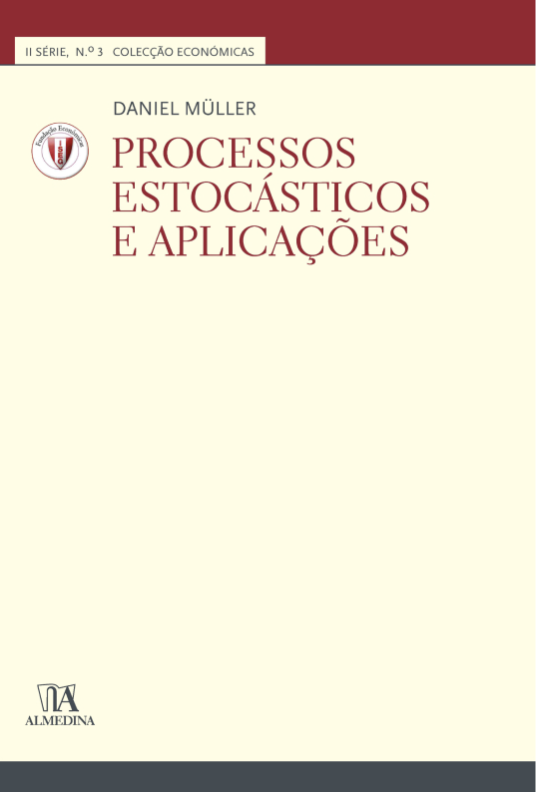
\includegraphics[width=0.2\linewidth]{figures/book1} \end{center}

\textbf{Secundária}

\begin{itemize}
\tightlist
\item
  Muller, D. (2011) Probabilidades e Processos Estocásticos. II Série, nº17, Coleção Económicas. Almedina.
\end{itemize}

\begin{center}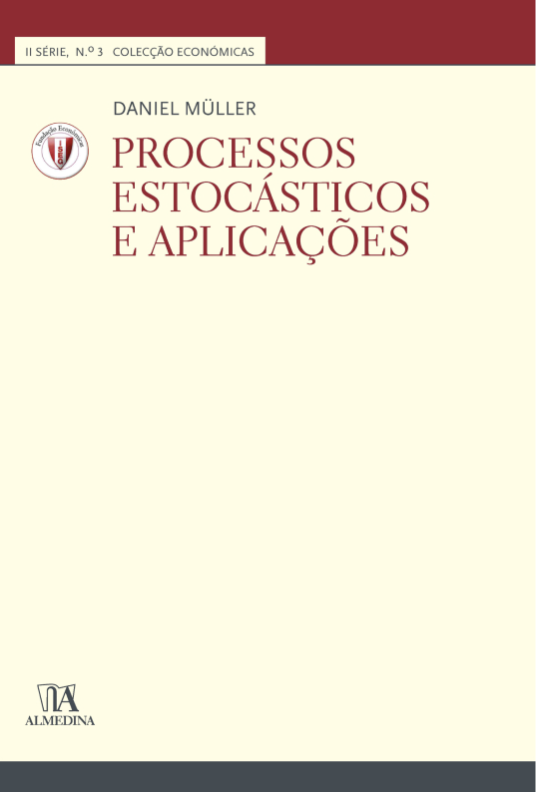
\includegraphics[width=0.2\linewidth]{figures/book1} \end{center}

\begin{itemize}
\tightlist
\item
  Taylor, H. M., Karlin, S. (1998) An Introduction to Stochastic Modeling (3rd Edition), Academic Press, New York.
\end{itemize}

\begin{center}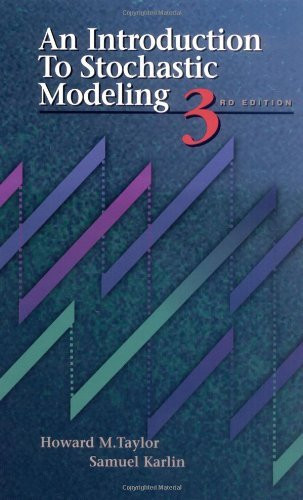
\includegraphics[width=0.2\linewidth]{figures/book3} \end{center}

\vfill

\(\,\)

\(\,\)

\(\,\)

\(\,\)

\textbf{Todos os direitos reservados. É expressamente proibida a reprodução, cópia, distribuição, comunicação pública, transformação ou qualquer outra forma de utilização, total ou parcial, dos conteúdos deste sítio, incluindo textos, código e imagens, sem autorização prévia e por escrito do autor. Qualquer utilização não autorizada constitui violação dos direitos de autor e poderá dar lugar à responsabilidade civil e criminal nos termos da lei em vigor.}

2025 \textbar{} Nuno M. Brites \textbar{}
\href{mailto:nbrites@iseg.ulisboa.pt}{\nolinkurl{nbrites@iseg.ulisboa.pt}}

\end{document}
